\documentclass{classes/fiboThesis}
\usepackage{tabularx}
\usepackage{graphicx}
\usepackage{adjustbox}
\usepackage{lscape}

\begin{document}
\title{Goggle : People Video Analytics and Deep Learning Platform}
\titleTH{-- ชื่อภาษาไทย --}

\author{นายปฐมพงศ์ สินธุ์งาม}
\authorTwo{นายศุภกร เบญจวิกรัย}
\authorThree{นายอุกฤษฎ์ เลิศวรรณาการ}

\majoradvisor{นายธนัชชา ชูพจน์เจริญ}
\coadvisor{รศ.ดร.ชิต เหล่าวัฒนา}
\committeeOne{ดร.อาบทิพย์ ธีรวงศ์กิจ}
\committeeTwo{ดร.ปิติวุฒญ์ ธีรกิตติกุล}
\committeeThree{ดร.สุภชัย วงศ์บุณย์ยง}

\academicyearTH{2562}

\maketitle
\frontmatter
\maketitleinner
\makeapproval
% ************************** Thesis Abstract **********************************
\begin{abstract}
งานวิทยานิพนธ์นี้เป็นงานที่เกี่ยวกับการออกแบบและจัดทำ labeling tool และระบบวิเคราะห์การกระทำของมนุษย์
โดยใช้ชื่อว่า Goggle แพลตฟอร์มการเรียนรู้เชิงลึกและระบบวิเคราะห์การกระทำของมนุษย์ 
และมีจุดประสงค์เพื่อให้ผู้พัฒนาสามารถใช้งาน labeling tool ในการสร้างชุดข้อมูลได้ง่ายและสะดวกขึ้น
ภาพรวมของวิทยานิพนธ์นี้จะแบ่งออกเป็นทั้งหมดสามส่วน คือ 
ส่วนแรกเป็นส่วนของการศึกษาหาความเป็นไปได้ และเทคโนโลยีในปัจจุบันที่เกี่ยวกับการสร้างแอพพลิเคชั่น 
และการจดจำการกระทำของมนุษย์ด้วยปัญญาประดิษฐ์ เพื่อนำมาประยุกต์ใช้กับงานวิจัยนี้
ส่วนที่สองเป็นส่วนของการออกแบบและสร้างแอพพลิเคชั่นที่ใช้ในการสร้างชุดข้อมูลสำหรับการเทรนโมเดลจากวิดีโอ
และส่วนสุดท้ายเป็นส่วนของการออกแบบและสร้างระบบวิเคราะห์การกระทำของมนุษย์ได้โดยจะกำหนดไว้ในบทนำ
\vfill
\paragraph*{คำสำคัญ :} ระบบวิเคราะห์การกระทำของมนุษย์ / labeling tool / Goggle
\vfill
\end{abstract}
% ************************** Thesis Acknowledgements **************************
% \majoradvisor{นายธนัชชา ชูพจน์เจริญ}
% \coadvisor{รศ.ดร.ชิต เหล่าวัฒนา}
% \committeeOne{ดร.อาบทิพย์ ธีรวงศ์กิจ}
% \committeeTwo{ดร.ปิติวุฒญ์ ธีรกิตติกุล}
% \committeeThree{ดร.สุภชัย วงศ์บุณย์ยง}
\begin{acknowledgements}
ขอขอบพระคุณ ดร.วราสิณี ฉายแสงมงคล อาจารย์ที่ปรึกษาวิทยานิพนธ์หลัก
ที่ได้สละเวลามาให้คำปรึกษา ชี้แนะแนวทาง ให้ความรู้ในด้านต่างๆ ที่จำเป็นต่องานวิจัย 
รวมถึงการให้การสนับสนุนในเรื่องอุปกรณ์ในการทำวิจัย ช่วยตรวจและแก้ไขวิทยานิพนธ์ให้เป็นไปอย่างสมบูรณ์
ตลอดจนกรุณาให้เกียรติเป็นประธานกรรมการสอบวิทยานิพนธ์

ขอขอบพระคุณอาจารย์อาจารย์ บวรศักดิ์ สกุลเกื้อกูลสุข ที่กรุณาให้เกียรติเป็นกรรมการสอบวิทยานิพนธ์ 
ให้คำแนะนำที่เป็นประโยชน์ต่อการวิจัย และการแก้ไขปรับปรุงงานวิจัย ตลอดจนตรวจแก้วิทยานิพนธ์ให้ดำเนินไปอย่างสมบูรณ์

ขอขอบพระคุณอาจารย์ ดร.บุญฑริกา เกษมสันติธรรม ที่กรุณาให้เกียรติเป็นกรรมการสอบวิทยานิพนธ์ 
ให้คำแนะนำที่เป็นประโยชน์ต่อการวิจัย และการแก้ไขปรับปรุงงานวิจัย ตลอดจนตรวจแก้วิทยานิพนธ์ให้ดำเนินไปอย่างสมบูรณ์

ขอขอบพระคุณคณาจารย์ และบุคลากรในสถาบันวิทยาการหุ่นยนต์ภาคสนามทุกท่าน
ที่ได้ให้คำปรึกษาและช่วยเหลือด้านสถานที่พร้อมทั้งสิ่งอำนวยความสะดวกต่างๆ ในระหว่างการทำวิทยานิพนธ์

ขอขอบคุณนักศึกษาปริญญาตรี สถาบันวิทยาการหุ่นยนต์ภาคสนามทุกท่าน
ที่ได้ให้คำแนะนำ ถามไถ่ และเป็นกำลังใจมาโดยตลอด

และสุดท้ายนี้ ขอน้อมรำลึกถึงพระคุณบิดา มารดา และครอบครัว ที่ส่งเสริมให้กำลังใจ
และให้การสนับสนุนในเรื่องต่างๆ จนกระทั่งข้าพเจ้าประสบความสำเร็จในการศึกษา
\end{acknowledgements}

\tableofcontents
\listoffigures
\listoftables
\input{pages/symbols}
% ************************** Thesis Abbreviations **************************
\begin{abbreviations}
    \noindent
    \begin{tabular*}{\textwidth}{@{}p{0.3\textwidth}p{0.8\textwidth}@{}}
        {AVA} & {Atomic Visual Actions} \\
        {Artificial intelligence} & {ปัญญาประดิษฐ์} \\
        {Machine learning model} & {โมเดลปัญญาประดิษฐ์} \\
        {Label} & {คำกำกับที่บ่งบอกถึงคุณลักษณะของสิ่งที่สนใจ} \\
        {Labeling} & {การสร้างคำกำกับคุณลักษณะ} \\
        {Human action classification} & {การจำแนกการกระทำของมนุษย์} \\
        {Video labeling} & {การสร้างคำกำกับคุณลักษณะภายในวิดิโอ} \\
        {Video analytics} & {การวิเคราะห์ผลวิดิโอ} \\
        {Uniform label distribution} & {การที่มีจำนวนตัวอย่างภายในคำกำกับเท่ากันทุกประเภท} \\
        {KMUTT} & {King Mongkut's University of Technology Thonburi} \\
    \end{tabular*}
\end{abbreviations}


\mainmatter
\chapter{บทนำ}
%%%%%%%%%%%%%%%%%%%%%%%%%%%%%%%%%%%%%%%%%%%%%%%%%%%%%%%%%%%%%%%%%%%%%%%%%%%%%%%
\section{ที่มาและความสำคัญ}
บริษัท เพอเซ็ปทรา ดำเนินธุรกิจเกี่ยวกับการให้บริการและคำปรึกษาเกี่ยวกับปัญญาประดิษฐ์(artificial intelligence)
โดยลูกค้านั้นมีความต้องการที่จะให้ทางบริษัทสร้างปัญญาประดิษฐ์เพื่อนำไปใช้งานหรือแก้ปัญหาที่ต่างกันออกไป 
ทำให้การสร้างปัญญาประดิษฐ์ ซึ่งการที่จะตอบสนองความต้องการของลูกค้าเหล่านั้น 
จำเป็นต้องมีชุดข้อมูล(dataset)ที่เหมาะสมกับปัญหานั้นๆ เช่น ร้านขายของแห่งหนึ่งต้องการรู้ว่าในแต่ละวันมีลูกค้าเดินเข้าร้านกี่คน เป็นผู้ชายกี่คน เป็นผู้หญิงกี่คน เป็นต้น
ซึ่งการจะสร้างปัญญาประดิษฐ์ที่เหมาะสมกับการแก้ปัญหานี้ ก็จำเป็นต้องมีชุดข้อมูลที่เหมาะสม บางครั้งอาจต้องใช้มนุษย์ในการสร้างขึ้นมาโดยการเก็บข้อมูลวิดีโอ 
และลงมือสร้างชุดข้อมูลจากวิดีโอที่ได้ด้วยตัวเอง ซึ่งหากมีวิดีโอเป็นจำนวนมาก การใช้มนุษย์ในการสร้างชุดข้อมูลนั้นอาจจะต้องใช้มนุษย์เป็นจำนวนมาก 
และก่อให้เกิดภาระแก่มนุษย์ อีกทั้งยังเป็นงานที่ลำบาก และน่าเบื่อ

ทางคณะผู้วิจัยจึงมีความต้องการที่จะออกแบบและสร้างแอพพลิเคชั่น labeling tool สำหรับสร้างชุดข้อมูลจากวิดีโอ เพื่อช่วยแบ่งเบาภาระของผู้พัฒนาในการสร้างชุดข้อมูล 
เพื่อนำชุดข้อมูลเหล่านี้ไปสร้างโมเดลปัญญาประดิษฐ์สำหรับใช้แก้ปัญหาที่ลูกค้าต้องการ โดยโครงการสหกิจนี้เน้นศึกษาเกี่ยวกับการวิเคราะห์และจดจำการกระทำของมนุษย์ภายในสำนักงานจากภาพเคลื่อนไหวเป็นหลัก

%%%%%%%%%%%%%%%%%%%%%%%%%%%%%%%%%%%%%%%%%%%%%%%%%%%%%%%%%%%%%%%%%%%%%%%%%%%%%%%
\section{วัตถุประสงค์}
\begin{enumerate}
	\setlength\itemsep{-0.25em}
	\item เพื่อออกแบบ และสร้างระบบที่สามารถตรวจจับมนุษย์ และจดจำการกระทำพื้นฐานของมนุษย์ภายในสำนักงาน 
	ประกอบด้วย ยืน นั่ง เดิน เล่นโทรศัพท์ กินข้าว พูดคุย นอน โดยใช้ปัญญาประดิษฐ์ประมวลผล
	\item เพื่อสร้างเครื่องมือที่สามารถการสร้างชุดข้อมูลสำหรับการสร้างโมเดลปัญญาประดิษฐ์ในการจดจำการกระทำของมนุษย์ ให้สามารถใช้งานได้ง่าย 
	สะดวกสบายมากขึ้น และมีประสิทธิภาพที่สูงกว่าเครื่องมือตัวอื่นในปัจจุบัน
\end{enumerate}

%%%%%%%%%%%%%%%%%%%%%%%%%%%%%%%%%%%%%%%%%%%%%%%%%%%%%%%%%%%%%%%%%%%%%%%%%%%%%%%

\section{ประโยชน์ที่คาดว่าจะได้รับ}
\begin{enumerate}
	\setlength\itemsep{-0.25em}
	\item ออกแบบและสร้างแอพพลิเคชั่น labeling tool โดยมีปัญญาประดิษฐ์เข้ามาช่วย ที่สามารถสร้าง label สำหรับนำไปใช้สร้างโมเดลปัญญาประดิษฐ์ได้
	\item ออกแบบและสร้างต้นแบบของแพลตฟอร์มวิเคราะห์การกระทำมนุษย์ โดยงานวิจัยนี้จะมุ่งเน้นการประมวลผลวิดีโอแล้วสร้างรายงานเกี่ยวกับกิจกรรมของมนุษย์ภายในสำนักในวิดีโอได้
	\item สร้างและทดสอบโมเดลปัญญาประดิษฐ์สำหรับการจดจำการกระทำของมนุษย์อย่างน้อย 2 โมเดล
\end{enumerate}
\clearpage

%%%%%%%%%%%%%%%%%%%%%%%%%%%%%%%%%%%%%%%%%%%%%%%%%%%%%%%%%%%%%%%%%%%%%%%%%%%%%%%
\section{ขอบเขตการดำเนินงาน}
\begin{enumerate}
	\setlength\itemsep{-0.25em}
	\item Labeling tool ต้องสามารถตัดวิดิโอช่วงเวลาที่ไม่มีมนุษย์อยู่ออกได้อัตโนมัติโดยใช้ปัญญาประดิษฐ์
	\item Labeling tool สามารถระบุตำแหน่งมนุษย์แต่ละคนในวิดีโอได้และสามารถระบุการกระทำของมนุษย์ในวิดีโอได้ 
	โดยการกระทำที่กำหนดจะประกอบไปด้วยกระทำได้แก่ ยืน นั่ง ใช้คอมพิวเตอร์ เล่นโทรศัพท์ เดิน กินข้าว 
	\item ชุดข้อมูลผลลัพธ์ที่ได้จาก labeling tool ต้องสามารถนำไปใช้ในการสร้างโมเดลปัญญาประดิษฐ์ต่อได้
	\item สร้างแอพพลิเคชั่น labeling tool ด้วยภาษาไพธอน(Python)
	\item ออกแบบและสร้างแอพลิเคชั่น labeling tool ที่มนุษย์สามารถทำงานร่วมกับปัญญาประดิษฐ์ได้
	\item สร้างโมเดลปัญญาประดิษฐ์สำหรับการจดจำการกระทำของมนุษย์อย่างน้อย 2 โมเดล ที่สามารถระบุการกระทำของมนุษย์ตามที่กำหนดไว้ได้ในข้อ 2. 
	เพื่อนำไปใช้ในการสร้างระบบวิเคราะห์การกระทำมนุษย์ภายในสำนักงาน
	\item ระบบวิเคราะห์การกระทำมนุษย์ต้องสามารถนำวิดีโอมาวิเคราะห์ข้อมูลการกระทำและตำแหน่งของมนุษย์แต่ละคน แล้วนำข้อมูลเหล่านั้นไปสร้างรายงานออกมาได้
	\item ความละเอียดอย่างต่ำของวิดีโอต้องมากกว่า 640 x 480 (กว้าง x สูง)
	\item วิดีโอจะต้องมีเฟรมเรทต่อวินาที(fps) อย่างต่ำ 10 fps
\end{enumerate}

%%%%%%%%%%%%%%%%%%%%%%%%%%%%%%%%%%%%%%%%%%%%%%%%%%%%%%%%%%%%%%%%%%%%%%%%%%%%%%%
\section{ภาพรวมของระบบและขั้นตอนการดำเนินงาน}
งานวิจัยนี้การดำเนินงานวิจัยถูกแบ่งออกเป็นสองส่วน คือ ส่วนที่หนึ่งส่วนเครื่องมือสำหรับการเตรียมชุดข้อมูล (dataset) เป็นส่วนที่ทำเครื่องมือสำหรับช่วยผู้พัฒนาในการสร้างชุดข้อมูล และส่วนที่สองนำชุดข้อมูลไปสร้างโมเดล
\subsection*{ศึกษาค้นคว้าเอกสารและงานวิจัยที่เกี่ยวข้อง}
\begin{enumerate}\setlength\itemsep{-0.25em}
	\item ศึกษาเกี่ยวกับการวิเคราะห์ผลวิดิโอ (video analytics)
	\item ศึกษาเกี่ยวกับชุดข้อมูลสำหรับการวิเคราะห์ผลวิดิโอ
	\item ศึกษาเกี่ยวกับโมเดลใช้ในการวิเคราะห์ผลวิดิโอ
	\item ศึกษาเครื่องมือที่ใช้สำหรับช่วยสร้างชุดข้อมูล
\end{enumerate}
\subsection*{ส่วนเครื่องมือสำหรับการเตรียมชุดข้อมูล (dataset)}
\begin{enumerate}\setlength\itemsep{-0.25em}
	\item ออกแบบหน้าต่างของแอพพลิเคชั่น
	\item สร้างระบบของแอพพลิเคชั่น
	\item ทดสอบการทำงานของแอพพลิเคชั่น
\end{enumerate}
\subsection*{ส่วนนำชุดข้อมูลไปสร้างโมเดล}
\begin{enumerate}\setlength\itemsep{-0.25em}
	\item สร้างชุดข้อมูลสำหรับสร้างโมเดล
	\item สร้างโมเดลสำหรับการทำนายการกระทำของมนุษย์
	\item ทดสอบการทำงานของโมเดล
\end{enumerate}
\clearpage
%%%%%%%%%%%%%%%%%%%%%%%%%%%%%%%%%%%%%%%%%%%%%%%%%%%%%%%%%%%%%%%%%%%%%%%%%%%%%%%
\section{Gantt chart}แผนการทำงานของคณะวิจัยจะแบ่งออกเป็น 3 ช่วง ซึ่งในแต่ละช่วงจะมี task ดังนี้
\begin{enumerate}
	\item Phase 1 :  ศึกษาข้อมูลเกี่ยวกับการทำวิเคราะห์วิดีโอ(video analytics) และเครื่องมือที่ใช้ในการทำโครงการวิจัย
		\begin{enumerate}\setlength\itemsep{-0.25em}
			\item task 1 	ศึกษา และ ทดลองใช้เทคนิคที่เกี่ยวข้องกับการวิเคราะห์วิดีโอ(video analytics)
			\item task2	รวบรวมชุดข้อมูลสำหรับการทำ human action recognition
		\end{enumerate}
	\item Phase 2 :  สร้างและออกแบบแอพพลิเคชั่นโดยจะประกอบด้วยงานในส่วนหลักๆ คือ
		\begin{enumerate}\setlength\itemsep{-0.25em}
			\item task3	โมเดลสำหรับวิเคราะห์ผลการกระทำของมนุษย์
			\item task4	หน้าต่าง UI
		\end{enumerate}
	\item Phase 3 : ปรับปรุงและแก้ไขปัญหา ทำให้แอพพลเคชั่นสามารถนำไปใช้งานได้จริง
\end{enumerate}

%%%%%%%%%%%%%%%%%%%%%%%%%%%%%%%%%%%%%%%%%%%%%%%%%%%%%%%%%%%%%%%%%%%%%%%%%%%%%%%
\section{Milestones}จะมีการกำหนด milestones ทั้งหมด 3 ครั้ง คือ
\begin{enumerate}
	\item Milestone  1  วันที่ 12  มิถุนายน  2562
		\begin{enumerate}\setlength\itemsep{-0.25em}
			\item ศึกษางานวิจัยที่เกี่ยวข้องกับการวิเคราะห์วิดีโอ(video analytics) ต่าง ๆ  ได้แก่ Youtube-8M , Moment in time , AVA
		\end{enumerate}
	\item Milestone  2  วันที่ 14  สิงหาคม 2562
		\begin{enumerate}\setlength\itemsep{-0.25em}
			\item สร้างหน้าต่าง UI ครบสมบูรณ์
			\item ความคืบหน้าของโมเดลมากกว่า 50 \%-symbol
			\item ฟังก์ชั่นการทำงานของแอพพลิเคชั่นสามารถทำงานได้มากกว่า 50 \%-symbol
		\end{enumerate}
	\item Milestone  3  วันที่ 15  ตุลาคม 2562
		\begin{enumerate}\setlength\itemsep{-0.25em}
			\item แอพพลิเคชั่นสามารถทำงานได้ครบกระบวนการ
			\item ได้โมเดลสามารถทำนายการกระทำของมนุษย์ได้
		\end{enumerate}
\end{enumerate}




%% ************************** Thesis Chapter2 **********************************
\clearpage
\chapter{ทฤษฎี/การวิจัยที่เกี่ยวข้อง}
ในส่วนของงานที่เกี่ยวข้องกับการวิเคราะห์วิดีโอในปัจจุบันนั้นมีความหลากหลายของวิธีในการทำ ผู้วิจัยจึงจำเป็นต้องศึกษาองค์ความรู้และงานวิจัยที่ตรงกับวัตถุประสงค์ของงาน เพื่อศึกษาและเป็นแนวทางในการประยุกต์ใช้สร้าง Video analytics platform ซึ่งหัวข้อที่ผู้วิจัยได้ไปศึกษามา มีดังต่อไปนี้
\begin{enumerate}
	\setlength\itemsep{-0.25em}
	\item การวิเคราะห์ผลวิดีโอ
	\begin{enumerate}	
		\item การตรวจจับวัตถุ
		\item การทำนายตำแหน่งถัดไปของวัตถุ
		\item การระบุตัวตนของบุคคล
		\item การจดจำการกระทำ
	\end{enumerate}
	\setlength\itemsep{-0.25em}
	\item เครื่องมือสำหรับการวิเคราะห์ผลวิดีโอ
	\begin{enumerate}	
		\item Machine learning model
		\item เครื่องมือสำหรับสร้างชุดข้อมูล
	\end{enumerate}
\end{enumerate}

\section{การวิเคราะห์ผลวิดีโอ}
ในส่วนของงานวิจัยนี้สิ่งที่สนใจ คือ ข้อมูลการกระทำของมนุษย์แต่ละคนภายในวิดีโอ เพื่อที่จะได้ผลลัพธ์ที่มีประสิทธิภาพออกมาเป็นข้อมูลของสิ่งที่สนใจ เช่น จำนวนคนที่เดินผ่านกล้อง 
หรือทิศทางการเดินของคนในวิดีโอ จึงจำเป็นต้องใช้การประมวลผลวิดีโอเพื่อที่จะสกัดสิ่งที่สนใจออกมาจากวิดีโอ ซึ่งการประมวลผลวิดีโอมีหลากหลายกระบวนการ 
โดยในแต่ละกระบวนการจะมีจุดประสงค์ของการทำและผลลัพธ์หลังการประมวลผลที่แตกต่างกัน ในหัวข้อนี้จะมาอธิบายถึงกระบวนการในการประมวลผลของวิดีโอและผลลัพธ์ของกระบวนการนั้น
\subsection{การตรวจจับวัตถุ}
การตรวจจับวัตถุนั้นเป็นหนึ่งในกระบวนการวิเคราะห์ผลของวิดีโอ กล่าวคือกระบวนการที่ผู้วิจัยจะต้องทำการระบุสิ่งที่สนใจว่า คืออะไร อยู่ที่ตำแหน่งใด 	การตรวจจับวัตถุถูกค้นพบเมื่อนานมาแล้ว และในปัจจุบันนั้นสามารถทำได้หลากหลายวิธี โดยภายในบทความนี้จะสรุปใจความสำคัญของวิธีการต่างในการตรวจจับวัตถุ เช่น Sliding Window , Brute Force Search , R-CNN , Fast-RCNN , Faster-RCNN , YOLO , SSD 
\begin{enumerate}
		\item Sliding Window วิธีการที่เปรียบเสมือนมีหน้าต่าง (kernel) ค่อยๆเลื่อนไปยังแต่ละพิกเซลบนรูป ซึ่งก่อนการเลื่อนของหน้าต่างแต่ละครั้ง จะนำส่วนของรูปภาพที่ถูกหน้าต่างทับอยู่ไปทำนายว่าใช่วัตถุที่เราต้องการหรือไม่ จากนั้นจึงค่อยเลื่อนถัดไป โดยจะทำกระบวนการแบบนี้จนครบทั้งรูปภาพ
	\item Brute Force Search ถูกสร้างขึ้นมาเพื่อแก้ปัญหาขนาดของหน้าต่างไม่ตรงกับขนาดของวัตถุที่อยู่ในภาพทำให้มีโอกาสที่จะไม่พบวัตถุ โดยหลักการของวิธีการนี้ คือ การย่อ-ขยาย รูปภาพและนำเข้าในหลายๆอัตราส่วน ตั้งแต่ 0.1 เท่า จนถึง 2 เท่า แต่ข้อเสียของวิธีการนี้คือ มีการคำนวณพื้นที่ซ้ำๆ และ ใช้เวลานาน
	\item R-CNN ใช้อัลกอริทึ่ม Selective search เข้ามาช่วยในการเสนอพื้นที่ที่น่าจะมีวัตถุอยู่ทดแทนการค้นหาทุกๆตำแหน่ง จากนั้นก็นำรูปภาพในส่วนพื้นที่นั้นไปทำนายว่าวัตถุนั้นคืออะไร กรณีที่มีพื้นที่ที่อยู่ใกล้ๆวัตถุถูกเสนอเข้ามาเป็นจำนวนมากด้วย เราจะใช้ Non-Maximum Suppression (NMS) หรือการเลือกพื้นที่ที่ถูกทับซ้อนมากที่สุดในบริเวณนั้น
	\item Fast-RCNN จากวิธีการ R-CNN แต่ละพื้นที่จะถูกนำไปสกัดคุณลักษณะ และ ทำนายผลทีละพื้นที่่ ทำให้เสียเวลา โดย Faster-RCNN จะมีส่วนที่คล้ายกับ R-CNN ในส่วนการทำ Selective search หาพื้นที่ที่น่าจะมีวัตถุเหมือนเดิม แต่ Faster-RCNN จะนำรูปภาพทั้งรูปภาพไปสกัดคุณลักษณะ หลังจากที่ได้คุณลักษณะแล้ว นำพิกัดของพื้นที่ที่น่าจะมีวัตถุ บนรูปภาพที่ถูกสกัดคุณลักษณะแล้วของ ไปผ่าน ROI Pooling (การลดขนาดข้อมูลให้มีขนาดคงที่เพื่อเป็นอินพุทให้กับโมเดลในการทำนายผล)
	\item Faster-RCNN พัฒนาจาก Fast-RCNN โดยวิธีของ Faster-RCNN จะรวมในส่วนของ Selective search และ การทำงานอื่นๆให้อยู่ในโครงข่ายเดียวกัน สรุปคือการทำงานของโครงข่ายของ Faster-RCNN จะมีการทำงาน 3 อย่างหลักคือ 1) สกัดคุณลักษณะ 2) การเสนอส่วนที่น่าจะมีวัตถุอยู่ในรูปภาพ 3) หลังจากได้รูปภาพจากการสกัดคุณลักษณะ นำพิกัดของพื้นที่ที่น่าจะมีวัตถุ บนรูปภาพที่ถูกสกัดคุณลักษณะแล้วของ ไปผ่าน ROI Pooling
	\item YOLO เป็นวิธีการที่ใช้โครงข่ายประสาทแบบคอนโวลูชั่นเพียงตัวเดียวทำนายรูปภาพทั้งรูป โดยโครงข่ายจะแบ่งรูปภาพออกเป็นพื้นที่ และ ใช้ Fully-connected (เป็นโครงข่ายประสาทเทียมที่นำเอาคุณลักษณะมาทำนายผล) ทำนายตำแหน่งของกรอบสี่เหลี่ยมและหมวดหมู่ของกรอบสี่เหลี่ยมในแต่ละพื้นที่ไปพร้อมกัน 
	\item SSD ใช้โครงข่ายประสาทเทียมตัวเดียวเหมือนกับ YOLO แต่การออกแบบโครงสร้างแตกต่างกัน SSD จะใช้ VGG-16(เป็นโมเดล CNN ชนิดหนึ่ง) ในการสกัดคุณลักษณะ และ ใช้ Convolution layer ต่อกันหลายๆชั้นเพื่อลดมิติและความละเอียดทำให้ตรวจจับวัตถุในหลายๆขนาด ซึ่งในแต่ละชั้นจะได้ผลออกมาเป็น Convolution filter จากนั้นจะนำ Convolution filter ไปทำนายผลต่อ
\end{enumerate}

 



%ซึ่งในปัจจุบันการทำการตรวจจับวัตถุมักนำปัญญาประดิษฐ์มาใช้เนื่องจากมีความแม่นยำ และ ช่วยแบ่งเบาภาระของผู้วิจัยในการระบุสิ่งที่สุดใจภายในเฟรม ซึ่งโครงสร้างโมเดลปัญญาประดิษฐ์ของการตรวจจับวัตถุที่ผู้วิจัยสนใจมีดังนี้

\subsubsection*{YOLO}
\begin{figure}[!ht]
    \centering
    \includegraphics[width=0.7\textwidth]{chapter2/images/yolo.jpg}
    \caption{กระบวนการทำงานของโครงสร้างโมเดลปัญญาประดิษฐ์ของ YOLO}
    \label{fig:yolo}
\end{figure}

โครงสร้างโมเดลปัญญาประดิษฐ์ของ YOLO เป็นโครงสร้างที่มีความเร็วมาก มีความเร็วในการประมวลผลถึง 45 เฟรมต่อวิ ทำให้สามารถประมวลผลแบบเรียลไทม์ได้ นอกจากนั้นยังมีความแม่นยำ mAP มากกว่าโมเดลสำหรับตรวจจับวัตถุอื่นๆถึง 2 เท่า ซึ่งเหตุผลที่โครงสร้างโมเดลปัญญาประดิษฐ์ของ YOLO เร็วกว่าโมเดลปัญญาประดิษฐ์ตัวอื่นๆ เนื่องจาก มีแนวคิดที่ต่างออกไป คือ สำหรับการตรวจจับวัตถุในวิธีการก่อนหน้าจะใช้วิธีทำนายกรอบสี่เหลี่ยมก่อน แล้วจึงค่อยนำกรอบสี่เหลี่ยมไปทำนายว่าเป็นหมวดหมู่อะไร ซึ่ง YOLO มีวิธีการที่ต่างออกไป คือ ทำนายตำแหน่งของกรอบสี่เหลี่ยมและทำนายว่ากรอบสี่เหลี่ยมนั้นเป็นหมวดหมู่อะไรพร้อมกัน โดยใช้โครงข่ายประสาทแบบคอนโวลูชั่น ด้วยแนวคิดนี้จึงเป็นที่มาของชื่อ YOLO หรือ you only look once การมองแค่เพียงครั้งเดียว ซึ่งโครงสร้างโมเดลปัญญาประดิษฐ์ของ YOLO ที่ถูกใช้ในงานวิจัยนี้ประกอบไปด้วย 1) YOLOv3-tiny 2)YOLOv3 3) YOLOv3-spp	ซึ่งทั้ง 3 โครงสร้างจะมีความแตกต่างของโครงสร้างดังนี้
\begin{enumerate}
	\setlength\itemsep{-0.25em}
	\item YOLOv3-tiny ใช้ Max-Pooling layers ในขั้นตอนของการลดจำนวนข้อมูลตัวอย่าง
	\item YOLOv3 ใช้ Convolutional layers ในขั้นตอนของการลดจำนวนข้อมูลตัวอย่าง
	\item YOLOv3-spp ใช้ Convolutional layers+ฟีเจอร์ที่ดีที่สุดของ Max-Pooling layers ในขั้นตอนของการลดจำนวนข้อมูลตัวอย่าง
\end{enumerate}
%ข้อมูลผลการทำงานของโมเดลปัญญาประดิษฐ์สำหรับการทำการตรวจจับภาพบุคคล อ้างอิงข้อมูลจากเว็บไซต์ของ YOLO
%\begin{table}[!ht]
%	\begin{tabular}{|c|c|c|}
%		\hline
%		{}&{ความเร็วต่อรูปภาพ (มิลลิวินาที)}&{ความแม่นยำ (0.5 IoU mAP)}			\\
%		\hline
%		SSD Mobilenet v1 ppn	 		& 26				& 20														\\
%		YOLO-v3 320				& 22				& 51.5				\\	
%		YOLO-v3 tiny				& 4.5				& 33.1				\\
%		YOLO-v3 spp				& 50				& 60.6				\\	
%		Faster RCNN inceptrion v2		& 58				& 28		\\
%	\hline
%	\end{tabular}
%	\caption{ข้อมูลผลการทำงานของโมเดลปัญญาประดิษฐ์สำหรับการทำการตรวจจับภาพบุคคล อ้างอิงข้อมูลจากเว็บไซต์ของ YOLO}
%\end{table}



\subsection{ระบบติดตามการเคลื่อนไหวของวัตถุ}
การติดตามการเคลื่อนไหวของวัตถุ\textsuperscript{\cite{danelljan2014accurate}} คือระบบที่ใช้สำหรับการติดตามการเคลื่อนไหวของวัตถุที่สนใจที่อยู่ในรูปภาพ 
โดยใช้การคำนวณทางคณิตศาสตร์ และการประมวลผลภาพ (image processing) ทำให้การประมวลผลนั้นเร็วกว่าการใช้โมเดลปัญญาประดิษฐ์ ซึ่งอัลกอริทึมติดตามการเคลื่อนไหวที่นิยมใช้มีสองอัลกอริทึม
คือ correlation filter และ kalman filter ซึ่งหลักการของทั้งสองอัลกอริทึมนั้นจะแตกต่างกันโดยที่ correlation filter นั้นจะใช้พิกเซลของวัตถุในการคำนวณตำแหน่งถัดไปของวัตถุ 
และ kalman filter จะใช้ข้อมูลการเคลื่อนไหวในการคำนวณตำแหน่งถัดไปของวัตถุ ซึ่งจากการศึกษาในบทความ "Object Tracking using Correlation,
Kalman Filterand Fast Means Shift Algorithms"\textsuperscript{\cite{ali2006object}} kalman filter มีประสิทธิภาพที่สูงนั้นจะขึ้นอยู่กับข้อมูลที่ได้จากการวัด (measurement)
และความซับซ้อนในการเคลื่อนไหวของวัตถุ ในขณะที่ correlation นั้นมีประสิทธิภาพที่ด้อยกว่า kalman filter เพียงเล็กน้อยและสามารถติดตามการเคลื่อนไหวที่ซับซ้อนของวัตถุได้ดีกว่า 
(การเคลื่อนไหวที่ซับซ้อนหมายถึง การเคลื่อนไหวที่เกิดการเปลี่ยนทิศทางฉับพลันบ่อย) ผู้วิจัยจึงตัดสินใจเลือกใช้ correlation filter ในงานครั้งนี้
\begin{figure}[!ht]
	\centering
	\includegraphics[width=1\textwidth]{chapter2/images/track-concept.png}
		\caption[แนวคิดของระบบติดตามการเคลื่อนไหวของวัตถุ]{แนวคิดของระบบติดตามการเคลื่อนไหวของวัตถุ\textsuperscript{\cite{correlation_filter}}}
    	\label{fig:Track_concept}
\end{figure}

จากรูปที่ \ref{fig:Track_concept} เป็นหลักการในการติดตามการเคลื่อนไหวของวัตถุแบบ correlation filter โดยการนำรูปมาผ่านกระบวนการแปลงฟูรีเยร์ (fourier transform)
และนำมาคูณกับ correlation filter ซึ่งเป็นตัวกรองที่ใช้สำหรับการหาความสัมพันธ์กับวัตถุในภาพ จากนั้นทำการแปลงฟูรีเยร์ผกผัน (inverse fourier transform) 
เพื่อตรวจสอบว่าวัตถุในภาพนั้นอยู่ที่ตำแหน่งใด โดยมีการคำนวณเริ่มจากการหา correlation filter ที่ดีที่สุดโดยใช้วิธีลดผลรวมของข้อผิดพลาดกำลังสองให้น้อยที่สุดดังนี้

\begin{equation}
\epsilon = \left \| \sum_{l = 1}^{d} h^{l} \star f^{l} - g \right \|^2 + \lambda \sum_{l = 1}^{d}\left \| h^{l} \right \|^2
\end{equation}
โดยที่
\begin{conditions}
 \epsilon     	&   ค่าความคลาดเคลื่อน 							\\
 d      		&  จำนวนมิติของผังคุณลักษณะของภาพ  \\   
 h 			&  correlation filter								\\
\star 			&  circular correlation							\\
 f			&  พื้นที่สี่เหลี่ยมของวัตถุที่สนใจที่ได้จากการทำผังคุณลักษณะ	\\
 g			&  ผลลัพธ์ correlation ที่ต้องการของ f					\\
 \lambda   		&  regularization term
\end{conditions}

เมื่อพิจารณาจากรูปภาพเดียวในกรณีที่เวลา ($t$) เท่ากับ 1 จะสามารถจัดรูปสมการด้านบนได้ดังนี้ 

\begin{equation}
H^{l} = \frac{\bar{G}F^{l}}{\sum_{k=1}^{d}\bar{F^{k}}F^{k} + \lambda}
\end{equation}
\begin{equation}
H_{t}^{l} = \frac{A_{t}^{l}}{B_{t}}					
\end{equation}					
\begin{equation}
A_{t}^{l} = (1-\eta )A_{t-1}^{l} + \eta \bar{G_{t}}F_{t}^{l}
\end{equation}
\begin{equation}
B_{t} = (1-\eta )B_{t-1} + \eta \sum_{k=1}^{d}\bar{F_{t}^{k}}F_{t}^{k}
\end{equation}
\clearpage
โดยที่
\begin{conditions}
 H 		     	&   correlation filter								\\
 \eta      		&  อัตราการเรียนรู้						 		\\   
 \bar{G} 		&  g ที่ผ่านการทำ complex conjugation					\\
 F			&  พื้นที่สี่เหลี่ยมของวัตถุที่สนใจที่ได้จากการทำผังคุณลักษณะ	\\
 \bar{F}		&   f ที่ผ่านการทำ complex conjugation					\\
 t 	  		&  เวลา
\end{conditions}
จากสมการที่ได้มาจะสามารถทำให้หาตำแหน่งต่อไปของวัตถุที่สนใจได้ด้วยสมการต่อไปนี้
\begin{equation}
y = F^{-1}\left \{ \frac{\sum_{l = 1}^{d} \bar{A^{l}}Z^{l}}{B + \lambda} \right \}
\end{equation}
โดยที่
\begin{conditions}
 y 		     	&   correlation score										\\
 F^{-1}    		&  การแปลงฟูรีเยร์ผกผันแบบไม่ต่อเนื่อง (inverse discrete fourier transform)						\\   	
 \bar{A}^{l} 	&  $A^{l}$ ที่ผ่านการทำ complex conjugation				\\
 Z	 		&  พื้นที่สี่เหลี่ยมของวัตถุที่สนใจที่ได้จากการหาผังคุณลักษณะของภาพใหม่	
\end{conditions}
โดยค่าของ $y$ ที่ได้ออกมาจะทำให้รู้ถึงตำแหน่งของวัตถุที่สนใจได้ ณ ตำแหน่งที่ $y$ มีค่าสูงสุด

\subsection{ระบบระบุตัวตนของบุคคล}
การระบุตัวตนของบุคคล คือการระบุตัวตนของบุคคลภายในวิดีโอหรือระหว่างรูปภาพ สามารถนำมาประยุกต์ใช้ในด้านของการรักษาความปลอดภัย การตามหาบุคคล หรือการตรวจสอบการกระทำของบุคคลนั้นในวิดีโอได้
\par
การทำ การระบุตัวตนของบุคคล นั้นเป็นปัญหาที่ท้าทาย เนื่องจากคุณลักษณะทั่วไปของบุคคลในรูปภาพไม่เพียงพอต่อการระบุบุคคลภายในภาพว่าเป็นบุคคลคนเดียวกันได้ ซึ่งวิธีการที่ใช้สำหรับในการทำ การระบุตัวตนของบุคคล คือวิธีการที่เรียกว่า Dynamically Matching Local Information (DMLI) ที่สามารถจัดลายละเอียดข้อมูลของภาพที่เหมือนกันได้ และได้ประสิทธิภาพที่สูงออกมา
\par
โดยเริ่มต้นของการทำ การระบุตัวตนของบุคคล จะแบ่งภาพออกเป็นทั้งหมด 8 ส่วนและใช่คุณลักษณะของภาพมาทำ normalize ซึ่งจะช่วยในการลดความซ้ำซ้อนของข้อมูล ต่อมาข้อมูลที่ทำการ normalize มาใช้เปรียบเทียบความแตกต่างของคุณลักษณะของรูป หลังจากนั้นหาค่าเฉลี่ยของความแตกต่างออกมา ถ้าค่าที่ออกมาใกล้เคียง 0 จะพูดได้ว่าบุคคลในรูปนั้นเป็นบุคคลเดียวกัน
\clearpage
\subsection{ระบบจำแนกการกระทำของมนุษย์}
การจำแนกการกระทำเป็นกระบวนการในการทำนายการกระทำของมนุษย์หรือสิ่งที่สนใจอื่นๆที่เกิดการกระทำขึ้นภายในวิดีโอ 
โดยในหัวข้อนี้จะกล่าวถึงตั้งแต่ขั้นตอนการได้มาซึ่งชุดข้อมูลมีกระบวนการอย่างไร การนำโมเดลปัญญาประดิษฐ์มาใช้ในการจำแนกการกระทำ และการวัดผลของโมเดลปัญญาประดิษฐ์
โดยชุดข้อมูลที่ผู้วิจัยได้เลือกนำมาศึกษาจากชุดข้อมูลที่ถูกเป็นที่กล่าวถึงในปัจจุบัน และมีขนาดของชุดข้อมูลที่ใหญ่

จากบทความข้างต้นชุดข้อมูลที่เราได้เลือกนำมาใช้ได้แก่ YouTube-8M ,AVA ,Moment in Time โดยแต่ละชุดข้อมูลจะมีความแตกต่างกันในหลายๆด้าน 
แต่จะมีสิ่งที่เหมือนกัน คือ เป็นชุดข้อมูลสำหรับการวิเคราะห์ผลวิดีโอที่มีการสนใจการกระทำของมนุษย์ โดยในบทความนี้จะกล่าวถึงความแตกต่างในด้านต่างๆ 
เช่น เป้าหมายของแต่ละชุดข้อมูล ,วิธีการเก็บข้อมูลสำหรับชุดข้อมูล ,วิธีการสร้างคำกำกับ และรายละเอียดของชุดข้อมูล จากนั้นจะสรุปข้อมูลของแต่ละชุดข้อมูล

%%%%%%%%%%%%%%%%%%%%%%%%%%%%%%%%%%%%%%%%%%%%%%%%%%%%%%%%%%%%%%%%%%%%%%%%%%%%%
\subsubsection*{YouTube-8M} 
\begin{enumerate}
	\item {ชุดข้อมูล}
	\begin{enumerate}
		\setlength\itemsep{-0.25em}
		\item เป้าหมายของชุดข้อมูล : ใช้ทำนายธีมของวิดีโอ
		\item จำนวนของวิดีโอ : 8,264,650 วิดีโอ
		\item ความยาวเฉลี่ยของแต่ละวิดีโอ : 229.6 วินาที
		\item จำนวนของหมวดหมู่ของคำกำกับ : 4800 หมวดหมู่
		\item กฏในการรวบรวมข้อมูลดังนี้
		\begin{enumerate}
			\setlength\itemsep{-0.25em}
			\item ทุกๆหัวข้อต้องเป็นรูปธรรม
			\item ในแต่ละหัวข้อต้องมีจำนวนวิดีโอไม่น้อยกว่า 200 วิดีโอ
			\item ความยาวของวิดีโอต้องอยู่ระหว่าง 120 - 500 วินาที
		\end{enumerate}
		หลังจากได้กฏในการรวบรวมข้อมูลแล้ว ขั้นตอนต่อไปคือการสร้างคำศัพท์ที่ใช้ในการค้นหาข้อมูลวิดีโอจากใน YouTube 
		\item ขั้นตอนในการสร้างคำศัพท์มีดังนี้
		\begin{enumerate}
			\setlength\itemsep{-0.25em}
			\item กำหนดรายการที่อนุญาตหัวข้อที่เป็นรูปธรรมมา 25 ชนิด เช่น เกมส์ เป็นต้น
			\item กำหนดบัญชีดำหัวข้อที่คิดว่าไม่เป็นรูปธรรมไว้ เช่น software เป็นต้น
			\item รวบรวมหัวข้อที่มีอยู่ในรายการที่อนุญาตอย่างน้อย 1 หัวข้อ และต้องไม่มีอยู่ในบัญชีดำซึ่งจะทำให้ได้หัวข้อที่ต้องการมาประมาณ 50,000 หัวข้อ
			\item จากนั้นใช้ผู้ประเมินจำนวน 3 คน ในการคัดหัวข้อที่คิดว่าเป็นรูปธรรม และสามารถจดจำหรือเข้าใจได้ง่ายโดยไม่ต้องเชี่ยวชาญในด้านนั้นๆ 
			ซึ่งผู้ประเมิน ก็จะมีคำถามว่า “มันยากขนาดไหนถึงจะระบุได้ว่ามีหัวข้อดังกล่าวอยู่ในรูปหรือวิดีโอ โดยใช้เพียงแค่การมองเท่านั้น?” โดยแบ่งเป็นระดับดังนี้
			\begin{enumerate}
				\setlength\itemsep{-0.25em}
				\item บุคคลทั่วไปสามารถเข้าใจได้
				\item บุคคลทั่วไปที่ผ่านการอ่านบทความที่เกี่ยวข้องมาแล้วสามารถเข้าใจได้
				\item ต้องเชี่ยญในด้านใดซักด้านจึงจะเข้าใจได้
				\item เป็นไปไม่ได้ ถ้าไม่มีความรู้ที่ไม่ได้เป็นรูปธรรม
				\item ไม่เป็นรูปธรรม
			\end{enumerate}
			\item หลังจากคำถามข้างบนและการให้คะแนน จะทำการเก็บไว้เฉพาะหัวข้อที่มีคะแนนเฉลี่ยมากที่สุดอยู่ที่ประมาณ 2.5 คะแนนหรือต่ำกว่าเท่านั้น
			\item ทำให้สุดท้ายเหลือเพียงประมาณ 10,000 หัวข้อที่สามารถใช้ได้
			\item หลังจากได้หัวข้อที่คิดว่าเป็นรูปธรรมแล้วก็นำไปค้นหาและรวบรวมด้วย YouTube annotation system โดยมีขั้นตอนดังนี้										
			\begin{enumerate}
				\setlength\itemsep{-0.25em}
				\item สุ่มเลือกวิดีโอมา 10 ล้านวิดีโอ พร้อมกับหัวข้อของวิดีโอ โดยใช้กฏที่กำหนดไว้ เอาหัวข้อที่มีจำนวนวิดีโอน้อยกว่า 200 วิดีโอออก
				\item ทำให้เหลือจำนวนวิดีโออยู่ 8,264,650 วิดีโอ
				\item แยกออกเป็น 3 ส่วน Train set, Validate set และ Test set ในอัตราส่วน 70:20:10 ตามลำดับ
			\end{enumerate}
		\end{enumerate}
	\end{enumerate}
	\item {โมเดลปัญญาประดิษฐ์}
	\begin{enumerate}
		\setlength\itemsep{-0.25em}
		\item การเตรียมข้อมูล
			\begin{enumerate}  
				\item คุณลักษณะระดับเฟรม : การลดขนาดของข้อมูล เนื่องจากมีข้อมูลที่มีขนาดใหญ่ทำให้ใช้เวลาในการเปิดนาน ซึ่งกระบวนการนี้จะมีการลดความเร็วเฟรมต่อวินาที 
				เวกเตอร์ของคุณลักษณะ และแปลงข้อมูลจาก 32 บิท ให้เป็น 8 บิท
				\item คุณลักษณะระดับวิดีโอ : การแยกเวกเตอร์คุณลักษณะระดับวิดีโอจากคุณลักษณะระดับเฟรมซึ่งการทำแบบนี้ทำให้ได้ประโยชน์ 3 ข้อ 
				คือโมเดลทั่วไปที่ไม่ใช่โครงข่ายประสาทเทียใสามารถนำไปใช้งานได้ ขนาดข้อมูลเล็กลง และเหมาะกับการนำไปสร้างโมเดล domain adaptive มากขึ้น
			\end{enumerate}	
		\item โมเดลปัญญาประดิษฐ์ % --> เติมตรงนี้ <---
		\item เครื่องมือที่ใช้วัดผลสำหรับงานวิจัยนี้ คือ
		\begin{enumerate}
			\setlength\itemsep{-0.25em}
			\item Mean Average Precision (mAP)
			\item Hit@k
			\item Precision at equal recall rate (PERR)
		\end{enumerate}
		\item ความสามารถของ Machine learning model ในปัจจุบัน
		\begin{enumerate}
			\setlength\itemsep{-0.25em}
			\item 1 % --> เติมตรงนี้ <---
			\item 2 % --> เติมตรงนี้ <---
		\end{enumerate}
		\item ปัญหาที่พบ
		\begin{enumerate}
		\item เนื่องจากว่า YouTube-8M นั้นมีจำนวนข้อมูลที่เยอะมาก ทำให้ไม่สามารถตรวจสอบได้ทั้งหมดว่า ground-truth ของแต่ละวิดีโอนั้นมีความถูกต้องมากน้อยขนาดไหน ทำให้อาจเกิดข้อผิดพลาดได้ (ปัจจุบัน ปี 2019 YouTube-8M ได้มีการตรวจสอบข้อมูลอีกครั้ง เพื่อเพิ่มประสิทธิภาพของชุดข้อมูลซึ่งทำให้ปัจจุบันจำนวนข้อมูล และจำนวน category นั้นจะลดน้อยลงจากข้อมูลที่ใช้อ้างอิงในบทความ \footnote{YouTube-8M,https://arxiv.org/pdf/1609.08675.pdf} ข้างต้นที่ได้กล่าวมา)
	\end{enumerate}	

	\end{enumerate}	
	\end{enumerate}	

%%%%%%%%%%%%%%%%%%%%%%%%%%%%%%%%%%%%%%%%%%%%%%%%%%%%%%%%%%%%%%%%%%%%%%%%%%%%%
\subsubsection*{AVA}	
\begin{enumerate}
	\item {ชุดข้อมูล}
	\begin{enumerate}
		\item เป้าหมายของชุดข้อมูล : สนใจการกระทำของมนุษย์เป็นศูนย์กลาง
		\item จำนวนของวิดีโอ : 640 วิดีโอ
		\item ความยาวเฉลี่ยของแต่ละวิดีโอ : 15 นาที และ ถูกสุ่มตัวอย่างด้วยความถี่ 1 hz 
		\item จำนวนของหมวดหมู่ : 80 หมวดหมู่
		\item ขั้นตอนการเก็บข้อมูลสำหรับการทำชุดข้อมูลมีขั้นตอนการทำ 5 ขั้น คือ
	\begin{enumerate}
%
		\item การสร้างคำศัพท์การกระทำ จะมีหลัก 3 ข้อในการรวบรวมคำศัพท์ คือ
		\begin{enumerate}
			\item เก็บรวบรวมคำศัพท์ทั่วไปที่เกิดขึ้นในชีวิตประจำวัน
			\item จะต้องมีเอกลักษณ์ สามาถเห็นได้ชัดเจน เช่น การถือของ
			\item กำหนดรูปแบบของคำศัพท์ขึ้นมาและใช้ความรู้จากชุดข้อมูลอื่น ในการทำให้ได้หมวดหมู่ของการกระทำของมนุษย์ที่ครอบคลุมของชุดข้อมูล AVA
		\end{enumerate}

%
		\item  หนังและส่วนที่เลือกมาใช้วิดิโอที่ใช้ทำชุดข้อมูล AVA ทั้งหมดจะถูกนำมากจาก YouTube โดยเริ่มจากการรวบรวมเอารายชื่อของนักแสดงที่มีชื่อเสียง ซึ่งจะมีความหลากหลายของเชื้อชาติรวมกันอยู่ ซึ่งวิดิโอที่ถูกคัดเลือกจะมีเกณฑ์ดังนี้ คือ
			\begin{enumerate}
				\item วิดิโอต้องอยู่ในหมวด หนัง และ ละครโทรทัศน์
				\item จะต้องมีความยาวมากกว่า 30 นาที
				\item อัพโหลดเป็นเวลาอย่างน้อย 1 ปี
				\item มียอดวิวคนดูมากกว่า 1000 วิว
				\item ละเว้นวิดิโอบางประเภท เช่น ขาว-ดำ , ความละเอียดต่ำ , การ์ตูน , วิดิโอเกม
			\end{enumerate}
%
		\item  การตีกรอบบุคคลที่อยู่ภายในภาพ ประกอบด้วย 2 ขั้นตอน
			\begin{enumerate}
				\item สร้างกรอบสี่เหลี่ยม โดยใช้โมเดล Faster R-CNN สำหรับการตรวจจับมนุษย์
				\item นำมนุษย์มาใช้ในการตรวจสอบและแก้ไขกรอบสี่เหลี่ยมที่พลาดไป หรือ ตรวจจับผิด
			\end{enumerate}	
		\item  การเชื่อมของบุคคลในช่วงระยะเวลาสั้นๆของเฟรม 
\\
ทำการเชื่อมกรอบสี่เหลี่ยมที่อยู่ในช่วงเวลาเดียวกัน ซึ่งใช้วิธีการ track โดยยึดมนุษย์เป็นศูนย์กลาง ซึ่งจะนำมาคำนวณความใกล้เคียงกันโดยการจับคู่กรอบสี่เหลี่ยม และ ใช้ person embedding จากนั้นจะใช้ Hungarian algorithm ในการหาตัวเลือกที่ดีที่สุด

%
		\item การสร้างคำอธิบาย
\\
		การสร้างคำอธิบายของการกระทำจะถูกสร้างจากเหล่าคนที่เป็นผู้สร้างคำอธิบาย ซึ่งจะใช้หน้าต่างโปรแกรมสำหรับช่วยเหลือในการสร้างซึ่งใน 1 กรอบสี่เหลี่ยม สามารถมีคำอธิบายของการกระทำได้สูงสุดถึง 7 labels นอกจากนั้นสามารถตั้งสถานะบล็อกเนื้อหาที่ไม่เหมาะสม หรือ กรอบสี่เหลี่ยมที่ผิดพลาดได้อีกด้วย ในทางปฎิบัติจะสังเกตได้ว่ามันมีโอกาศผิดอย่างหลีกเลี่ยงไม่ได้ เมื่อต้องได้รับคำสั่งให้หาคำอธิบายของการกระทำที่ถูกต้องจาก 80 หมวดหมู่ จึงแบ่งขั้นตอนออกเป็น 2 ขั้นตอน คือ
		\begin{enumerate}
			\item ข้อเสนอของการกระทำสอบถามเหล่าผู้สร้างคำอธิบาย เพื่อสร้างข้อเสนอสำหรับคำอธิบายของการกระทำจากนั้นจับกลุ่มเข้าด้วยกัน ซึ่งจะทำให้มีโอกาสถูกต้องมากกว่าเป็นข้อเสนอแยกเดี่ยว
			\setlength\itemsep{-0.25em}
			\item ผู้ตรวจสอบข้อเสนอจะตรวจสอบข้อเสนอที่ได้จากขั้นตอนแรก ซึ่งในแต่ละวิดิโอคลิปจะใช้มนุษย์ในการตรวจสอบ 3 คน เมื่อคำอธิบายของการกระทำ ถูกตรวจสอบด้วยผู้ตรวจสอบข้อเสนออย่างน้อย 2 คน คำอธิบายของการกระทำนั้นจะถูกยึดเป็นคำอธิบายหลัก
		\end{enumerate}
	\end{enumerate}
	\end{enumerate}
	\item {Machine learning model}
	\begin{enumerate}
		\item Machine learning model ที่งานวิจัยนี้ใช้ two stream variant ซึ่งจะทำการประมวลผลทั้ง RGB flow และ optical flow และ เป็นโครงสร้างของ Faster RCNN ที่นำ Inception network เข้ามาใช้ 
		\item เครื่องมือที่ใช้วัดผลสำหรับงานวิจัยนี้ คือ ค่า IOU และ 3D IOUs 
		\begin{enumerate}
			\item ค่า IOU คือ ค่าที่ใช้วัดความสอดคล้องระหว่างสองเฟรม ซึ่งใช้สำหรับการวัดผลระดับเฟรม โดยจะเป็นการเทียบกันของกรอบสี่เหลี่ยมที่ตรวจเจอและกรอบสี่เหลี่ยมจริงของวัตถุ
			\item ค่า 3D IOUs คือ ค่าที่ใช้วัดความสอดคล้องระหว่างสองวิดีโอ ซึ่งใช้สำหรับการวัดผลระดับวิดิโอโดยเทียบกันของ ground truth tubes และ linked detection tubes  ซึ่งก็คือ การนำเอากรอบสี่เหลี่ยมจริงของวัตถุในเฟรมที่ติดต่อกันมาเรียงต่อกันเป็น tube และ linkded detection tube คือ การนำเอากรอบสี่เหลี่ยม (bounding box) ที่ตรวจเจอมาเรียงต่อกันเป็น tube
		\end{enumerate}	
		\item ความสามารถของ Machine learning model ในปัจจุบัน
		\begin{enumerate}
			\item จากการทดสอบการเทียบ Machine learning model ของงานวิจัยนี้และวิธีการอื่นๆ โดยนำไปทดสอบกับชุดข้อมูลวิดีโอ JHMDB และ UCF101-24 ได้ผลลัพธ์ออกมาดังนี้
	\begin{table}[!ht]
	\centering
	\begin{tabular}{|c|c|c|c|}
			\hline
			{Frame-mAP}&{JHMDB}&{UCF101-24}\\
			\hline
			Actionness 			& 39.9		& 	-						\\
			Peng w/o MR			& 56.9		& 64.8						\\
			Peng w/  MR 			& 58.5		& 65.7						\\
			ACT					& 65.7		& 69.5						\\
			\hline
			Out approach			& 73.3		& 76.3						\\
			\hline
		\end{tabular}
		\caption{ผลการทดลองของวิธีต่างๆบน Frame Level}
		\label{tab: transfer learning}
		\end{table}
	\end{enumerate}
		\item ปัญหาที่พบ

\end{enumerate}
\end{enumerate}
%%%%%%%%%%%%%%%%%%%%%%%%%%%%%%%%%%%%%%%%%%%%%%%%%%%%%%%%%%%%%%%%%%%%%%%%%%%%
\subsubsection*{Moment in Time}
\begin{enumerate}
	\item {ชุดข้อมูล}
	\begin{enumerate}
		\setlength\itemsep{-0.25em}
		\item เป้าหมายของชุดข้อมูล : สนใจการกระทำทุกการกระทำในวิดิโอ เช่น การกระทำของ คน สัตว์ สิ่งของ และ ปรากฎการณ์ธรรมชาติ 
		\item จำนวนของวิดีโอ : >1,000,000 วิดีโอ
		\item ความยาวเฉลี่ยของแต่ละวิดีโอ : 3 วินาที
		\item จำนวนของหมวดหมู่ : 339 หมวดหมู่
		\item วิธีการเก็บรวบรวมข้อมูล : 
	\begin{enumerate}
		\item เริ่มจากการรวบรวมคำ (verb) ที่มีการใช้อยู่ทั่วไปในชีวิตประจำวันมา 4,500 คำจาก VerbNet จากนั้นนำมาแบ่งกลุ่มคำ(verb) ที่มีความหมายใกล้เคียงกันโดยใช้ features จาก Propbank และ FrameNet โดยเก็บข้อมูลเป็นแบบ binary feature vector ซึ่งถ้าคำ (verb) ไหนมีความเกี่ยวข้องกับ feature ก็จะให้ค่าเป็น 1 ถ้าไม่เกี่ยวข้องกันจะให้ค่าเป็น 0 จากนั้นจึงใช้วิธี k-means clustering ในการแบ่งกลุ่ม เมื่อแบ่งกลุ่มแล้วจากนั้นจะเลือกคำ (verb) จากในแต่ละกลุ่มนั้น โดยคำ (verb) ที่เลือกมานั้นจะเป็นที่ใช้บ่อยที่สุดในกลุ่มนั้น และลบคำ (verb) นั้นออกจากกลุ่มทั้งหมด (คำ ๆ หนึ่งสามารถอยู่ได้หลายกลุ่ม) จากนั้นจะทำกระบวนการนี่ไปเรื่อย ๆ แต่คำ (verb) ที่เลือกมาจะต้องไม่มีความหมายคลุมเครือ ไม่สามารถมองเห็นหรือได้ยินได้ และต้องไม่มีความหมายเหมือนกับคำ (verb) ที่เคยเลือกมาก่อน จนสุดท้ายแล้วได้ออกมาที่ 339 class
		\item ต่อมาทำการหาชุดข้อมูลวิดีโอโดยจะตัดออกมาเพียง 3 วินาทีที่เกี่ยวข้องกับคำ (verb) ใน 339 class ที่เลือกมา จากวิดีโอ แหล่งต่างกัน 10 แหล่ง การตัดวิดีโอนั้นจะไม่ใช้พวก Video2Gif (โมเดลที่ระบุตำแหน่งของสิ่งที่น่าสนใจในวิดีโอ) เพราะจะทำให้เกิด bias ขึ้นจะเกิดขึ้นตอนสร้างโมเดลจากนั้นจะทำการส่งข้อมูลของคำ (verb) และวิดีโอที่ตัดไปยัง Amazon Mechanical Turk (AMT หรือตลาดแรงงาน) เพื่อทำการ label โดยพนักงานแต่ละคนของ AMT จะได้ 64 วิดีโอซึ่งเกี่ยวข้องกับคำ (verb) หนึ่ง และอีก 10 วิดีโอที่มีการทำ label อยู่แล้ว โดยวิดีโอที่มีการทำ label ถ้ามีพนักงานของ AMT ตอบเหมือนกันกับที่ทำ label ไว้เกิน 90\% ถึงจะนำเข้าไปรวมกับชุดข้อมูลส่วนอีก 64 วิดีโอถ้าเป็นของ training set จะต้องผ่านพนักงานของ AMT อย่างน้อย 3 ครั้ง และต้อง label เหมือนกัน 75\% ขึ้นไปถึงจะถือว่าเป็น label ที่ถูกต้อง ถ้าเป็นของ validation และ test set จะต้องผ่านพนักงานของ AMT อย่างน้อย 4 ครั้ง และต้อง label เหมือนกัน 85\% ขึ้นไป ที่ไม่ตั่งเกณฑ์ไว้ที่ 100\% เพราะจะทำให้วิดีโอนั้นยากเกินไปที่จะทำให้สามารถจำการกระทำได้	
	\end{enumerate}
\end{enumerate}
	\item การเตรียมข้อมูล
		\begin{enumerate}
			\item training set จะมี 802,264 วิดีโอ และมีวิดีโอในแต่ละ class อยู่ที่ 500 ถึง 5,000 วิดีโอ
			\item validation set จะมี 33,900 วิดีโอ และมีวิดีโอในแต่ละ class อยู่ที่ 100 วิดีโอ
			\item เริ่มการ preprocess จากแยกภาพRGB ออกมาจากวิดีโอ และทำการเปลี่ยนขนาดของภาพให้เป็น 340x256  pixel
			\item ใช้ TVL1 optical flow algorithm จาก opencv เพื่อลดข้อมูลรบกวนที่จะเกิดขึ้น
			\item ทำการแปลงค่าที่อยู่ใน optical flow ให้เป็นเลขจำนวนเต็ม(integer) เพื่อทำให้การคำนวณนั้นเร็วยิ่งขึ้น
			\item ปรับค่า displacement ใน optical flow ให้ค่าสูงสุดเป็น 15 ต่ำสุดเป็น 0 และทำการปรับขนาดให้เป็นช่วง 0-255
			\item เก็บข้อมูลออกมาในรูปแบบของ grayscale image เพื่อลดพื้นที่ ๆ ใช้เก็บข้อมูล
			\item แก้ปัญหาเรื่องการเคลื่อนไหวของกล้อง(camera motion) โดยการนำค่าเฉลี่ยของ เวกเตอร์(vector) ไปลบกับ displacement
			\item สุดท้ายจะเป็นสุ่มตัดภาพออกมาเพื่อเพิ่มจำนวนข้อมูล
		\end{enumerate}
	\item {Machine learning model}
	\begin{enumerate}
		\item ในงานวิจัยนี้มีการทดสอบ Machine learning model หลายอัน ซึ่ง Machine learning model ที่มีประสิทธิภาพการทำงานที่ดีที่สุดตาม 5 ลำดับแรกดังนี้
			\begin{enumerate}
				\item SVM				มีรูปแบบข้อมูลอินพุท คือ Spatial+Temporal+Auditory 	
				\item I3D 				มีรูปแบบข้อมูลอินพุท คือ Spatial+Temporal
				\item TRN-Multiscale		มีรูปแบบข้อมูลอินพุท คือ Spatial+Temporal
				\item TSN-2stream		มีรูปแบบข้อมูลอินพุท คือ Spatial+Temporal
				\item ResNet50-ImageNet	มีรูปแบบข้อมูลอินพุท คือ Spatial
			\end{enumerate}
		\item เครื่องมือที่ใช้วัดผลงานวิจัยนี้
			\begin{enumerate}
				\item Classification accuracy Top-1 , Top-5
			\end{enumerate}
		\item ความสามารถของ Machine learning model ในปัจจุบัน
			\begin{enumerate}
				\item ทำทดสอบ cross dataset transfer โดยการนำโมเดล ResNet50 I3D pretrained ลงทั้งบน Kinetics และ Moments in time และนำมาเทียบกับชุดข้อมูลอื่น โดยชุดข้อมูลแต่ละชุดจะมีการปรับ frame rate ของวิดีโอให้เป็น 5 fps เหมือนกัน
	\begin{table}[!ht]
		\centering
		\begin{tabular}{|c|c|c|c|}
			\hline
			{Pretrained}&\multicolumn{3}{c|}{Fine-Tuned}\\
			\cline{2-4}
			{}			& UCF		& HMDB		& Something			\\
			\hline
			\multirow{2}{*}{Kinetics}		& Top-1 : 92.6		& Top-1 : 62.0		& Top-1 : 48.6		\\
			{}						& Top-5 : 99.2		& Top-5 : 88.2		& Top-5 : 77.9		\\
			\hline
			\multirow{2}{*}{Moments}		& Top-1 : 91.9		& Top-1 : 65.9		& Top-1 : 50.0		\\
			{}						& Top-5 : 98.6		& Top-5 : 89.3		& Top-5 : 78.8		\\
			\hline
		\end{tabular}
		\caption{Data transfer performance ของโมเดล Resnet50 I3D}
		\label{tab: Data transfer performance ของโมเดล Resnet50 I3D}
	\end{table}
				\item จะเห็นได้ว่า Kinetics ให้ผลลัพท์ที่ดีกว่าใน UCF เพราะว่ามีการแชร์ class ด้วยกันอยู่หลายอย่าง ในขณะที่ HMDB นั้นมีการรวบรวม source จากหลายแหล่ง และมีจำนวน class ที่หลากหลายจึงทำให้มีความใกล้เคียงกับตัวข้อมูลของ Moments in time ดังนั้นจึงเทียบผลลัพท์จาก Something ซึ่งจะทำให้เห็นว่า Moments in time มีประสิทธิภาพที่ดีกว่าและวิดีโอที่มีความยาวมากกว่า 3 วินาทีจะไม่ส่งผลกระทบกับประสิทธิภาพของ Moments in time
		\end{enumerate}
	\end{enumerate}
	\item {ปัญหาที่พบ}
	\begin{enumerate}
		\item ผลลัพท์จากการทำนายด้วยโมเดลถ้าผ่านรูปภาพที่มีรายละเอียดเยอะจะทำให้การ ทำนายโอกาสผิดนั้นค่อนข้างสูง ซึ่งปัญหานี่สามารถทำให้เกิดน้อยลงด้วยการนำวิธี Class Activation Mapping(CAM) จะเป็นการเน้นรูปภาพในส่วนที่มีข้อมูลมากที่สุดและ ทำนายผลออกมา แต่ก็ยังมีจุดที่เป็นปัญหาอยู่ เช่น การกระที่เกิดขึ้นเร็วมาก (การลื่นล้ม) จะทำให้การทำนาย นั้นมีโอกาสผิดสูงขึ้น 
	\end{enumerate}


%%%%%%%%%%%%%%%%%%%%%%%%%%%%%%%%%%%%%%%%%%%%%%%%%%%%%%%%%%%%%%%%%%%%%%%%%%%%
\end{enumerate}		

\clearpage
\section{Labeling tools}
จากการค้นคว้าหาเครื่องมือในการสร้างคำกำกับข้อมูลเพื่อใช้เป็นแนวทางในการออกเครื่องมือกำกับข้อมูลด้วยปัญญาประดิษฐ์ พบเครื่องมือที่เปิดให้ใช้งานสาธารณะ 2 โปรแกรม 
คือ DarkLabel และ OpenLabeling โดยสรุปข้อมูลสำคัญได้ดังนี้ 
\subsubsection*{โปรแกรม DarkLabel\textsuperscript{\cite{dark}}}
เป็นโปรแกรมที่ช่วยในการทำนายคำกำกับและบันทึกในรูปแบบต่างๆ รองรับข้อมูลป้อนเข้าในรูปแบบไฟล์วิดีโอ avi, mpg หรือกลุ่มรูปภาพ มีขั้นตอนการสร้างคำกำกับดังนี้ 
\begin{enumerate}
	\setlength\itemsep{-0.25em}
	\item สร้างกรอบสี่เหลี่ยมครอบบริเวณวัตถุที่สนใจโดยใช้มนุษย์เป็นคนสร้าง
	\item กดปุ่ม Next และ Predict อย่างต่อเนื่อง เพื่อทำนายตำแหน่งต่อไปของกรอบสี่เหลี่ยมในเฟรมถัดๆไป จนกระทั่งการเกิดข้อผิดพลาด
	\item ลบกรอบสี่เหลี่ยมที่พลาด และเริ่มทำขั้นตอนที่ 1 ใหม่ อีกครั้งจนครบทุกเฟรมในวิดีโอ
\end{enumerate}

หลังจากที่ผู้วิจัยได้ทดลองใช้โปรแกรม DarkLabel พบว่าโปรแกรมมีการทำงานส่วนใหญ่ใช้มนุษย์ในการทำด้วยตัวเอง ซึ่งทำให้ใช้เวลาในการทำนาน

\begin{figure}[!ht]
	\centering
	\includegraphics[width=0.7\textwidth]{chapter2/images/darklabel.png}
		\caption{หน้าต่างการทำงานของโปรแกรม DarkLabel}
    	\label{fig:darklabel}
\end{figure}
\clearpage

\subsubsection*{โปรแกรม OpenLabeling\textsuperscript{\cite{open}}}
เป็นโปรแกรมที่ช่วยในการสร้างคำกำกับ โดยโปรแกรมจะมีการทำงานอยู่ 2 รูปแบบการทำงาน คือแบบทำด้วยตัวเอง (Mode Manual) และแบบอัตโนมัติ (Mode Auto) 
ซึ่งมีการทำงานแยกจากกันอย่างชัดเจน 

\begin{enumerate}
	\setlength\itemsep{-0.25em}
	\item การทำงานแบบอัตโนมัติ 
	\\ หลังจากป้อนวิดีโอเข้าไปในโปรแกรมแล้วมีขั้นตอนการสร้างคำกำกับดังนี้ 
   	\begin{enumerate}
	\setlength\itemsep{-0.25em}
		\item โปรแกรมจะทำงานอัตโนมัติโดยใช้โมเดลปัญญาประดิษฐ์ในการทำนายคีย์เฟรม (keyframe) 
		และทำนายตำแหน่งต่อไปของกรอบสี่เหลี่ยมในเฟรมถัดไปด้วยอัลกอริทึมที่ใช้การคำนวณคณิตศาสตร์และการประมวลผลภาพในภาพที่เหลือ ผลลัพธ์ที่ได้คือรูปภาพและไฟล์คำกำกับภาพ
 	\end{enumerate}
	\item การทำงานแบบทำด้วยตัวเอง 
	\\ หลังจากป้อนวิดีโอเข้าไปในโปรแกรมแล้วมีขั้นตอนการสร้างคำกำกับดังนี้ 
	\begin{enumerate}
	\setlength\itemsep{-0.25em}
		\item สร้างกรอบสี่เหลี่ยมขึ้นมาโดยใช้มนุษย์เป็นคนสร้าง
		\item กดปุ่มเพื่อทำนายตำแหน่งต่อไปของกรอบสี่เหลี่ยมในเฟรมถัดไป จนกระทั่งเกิดข้อผิดพลาด
		\item ลบกรอบสี่เหลี่ยมที่พลาด และเริ่มทำขั้นตอนที่ 1 อีกครั้งจนครบทุกเฟรมในวิดีโอ
 	\end{enumerate}
 \end{enumerate}

หลังจากที่ได้ทดลองใช้โปรแกรม OpenLabeling ทั้ง 2 รูปแบบการทำงานแล้วพบว่า การทำงานแบบอัตโนมัติไม่สามารถปรับแก้ไขสิ่งใดในระหว่างกระบวนการนั้น 
ทำให้หากเกิดกรณีที่โมเดลทำนายกรอบสี่เหลี่ยมพลาดจะไม่สามารถแก้ไขได้ และการทำงานแบบทำด้วยตัวเองผู้ใช้งานจะต้องสร้างกรอบสี่เหลี่ยมขึ้นมาเอง

\begin{figure}[!ht]
	\centering
	\includegraphics[width=0.7\textwidth]{chapter2/images/openlabel.png}
		\caption{หน้าต่างการทำงานของโปรแกรม OpenLabeling}
    	\label{fig:openlabel}
\end{figure}




\clearpage
%\section{ชุดข้อมูล}
%\subsubsection*{Youtube-8M}
YouTube-8M คือชุดข้อมูลวิดีโอที่เป็น multi-label ที่มีจำนวนวิดีโอเยอะที่สุด ซึ่งมีจำนวนมากถึง 8 ล้านวิดีโอ(ในปี 2016) โดยมีจุดมุ่งหมายหลักในการอธิบายธีมหลักของวิดีโอด้วยคำสั้นๆ เช่น ถ้าวิดีโอนั้นเป็นวิดีโอที่มี มนุษย์กำลังปั่นจักรยานบนถนนดินกับหน้าผา ชุดข้อมูลนี้จะอธิบายวิดีโอนี้ว่า mountain biking ซึ่งทำให้ YouTube-8M แตกต่างจากชุดข้อมูลวิดีโออื่นๆส่วนใหญ่ที่จะเน้น action หรือ activity ของมนุษย์ ซึ่งข้อมูลเชิงสถิติจะเป็นดังตารางที่ 1

\begin{figure}[!ht]
	\centering
	\includegraphics[width=1\textwidth]{chapter2/images/youtube-8m.png}
		\caption{ตัวอย่าง catagories ต่างๆของ YouTube-8M}
    	\label{fig:youtube-8m}
\end{figure}

\begin{table}[!ht]
\begin{tabular}{|c|c|c|c|}
		\hline
		{Number of video}&{Class of video}&{Avg. length of each video(s.)}&{Avg. class of video}				\\
		\hline
		8,264,650		& 4800		& 229.6		& 1.8											\\
		\hline
	\end{tabular}
	\caption{ข้อมูลเชิงสถิติของ YouTube-8M}
	\label{tab: ข้อมูลเชิงสถิติของ YouTube-8M}
\end{table}

\subsubsection*{1. วิธีการรวบรวมข้อมูล}
การเก็บข้อมูลของ YouTube-8M นั้นใช้เครื่องมือที่ชื่อว่า YouTube annotation system ในการเก็บรวบรวมข้อมูลโดยอาศัยผังความรู้(knowledge graph)ของ Google ในการค้นหาและรวบรวมข้อมูลในฐานข้อมูลของ YouTube
\begin{enumerate}
	\setlength\itemsep{-0.25em}
	\item กฏในการรวบรวมข้อมูลดังนี้
	\begin{enumerate}
		\setlength\itemsep{-0.25em}
		\item ทุกๆ หัวข้อต้องเป็นรูปธรรม
		\item ในแต่ละหัวข้อต้องมีจำนวนวิดีโอไม่น้อยกว่า 200 วิดีโอ
		\item ความยาวของวิดีโอต้องอยู่ระหว่าง 120 - 500 วินาที
	\end{enumerate}
หลังจากได้กฏในการรวบรวมข้อมูลแล้ว ขั้นตอนต่อไปคือการสร้างคำศัพท์(vocabulary)ที่ใช้ในการค้นหาข้อมูลวิดีโอจากใน YouTube 
	\item ขั้นตอนในการสร้างคำศัพท์มีดังนี้
	\begin{enumerate}
		\setlength\itemsep{-0.25em}
		\item กำหนด whitelist หัวข้อที่เป็นรูปธรรมมา 25 ชนิด เช่น game เป็นต้น
		\item กำหนด blacklist หัวข้อที่คิดว่าไม่เป็นรูปธรรมไว้ เช่น software เป็นต้น
		\item รวบรวมหัวข้อที่มีอยู่ใน whitelist อย่างน้อย 1 หัวข้อ และต้องไม่มีอยู่ใน blacklist ซึ่งจะทำให้ได้หัวข้อที่ต้องการมาประมาณ 50,000 หัวข้อ
		\item จากนั้นใช้ผู้ประเมินจำนวน 3 คน ในการคัดหัวข้อที่คิดว่าเป็นรูปธรรม และสามารถจดจำหรือเข้าใจได้ง่ายโดยไม่ต้องเชี่ยวชาญในด้านนั้นๆ ซึ่งผู้ประเมิน ก็จะมีคำถามว่า “ มันยากขนาดไหนถึงจะระบุได้ว่ามีหัวข้อดังกล่าวอยู่ในรูปหรือวิดีโอ โดยใช้เพียงแค่การมองรูปภาพเท่านั้น? ” โดยแบ่งเป็นระดับดังนี้
		\begin{enumerate}
			\setlength\itemsep{-0.25em}
			\item บุคคลทั่วไปสามารถเข้าใจได้
			\item บุคคลทั่วไปที่ผ่านการอ่านบทความที่เกี่ยวข้องมาแล้วสามารถเข้าใจได้
			\item ต้องเชี่ยญในด้านใดซักด้านจึงจะเข้าใจได้
			\item เป็นไปไม่ได้ ถ้าไม่มีความรู้ที่ไม่ได้เป็นรูปธรรม
			\item ไม่เป็นรูปธรรม
		\end{enumerate}
		\item หลังจากคำถามข้างบนและการให้คะแนน จะทำการเก็บไว้เฉพาะหัวข้อที่มีคะแนนเฉลี่ยมากที่สุดอยู่ที่ประมาณ 2.5 คะแนนเท่านั้น
		\item ทำให้สุดท้ายเหลือเพียงประมาณ 10,000 หัวข้อที่สามารถใช้ได้
		\item หลังจากได้หัวข้อที่คิดว่าเป็นรูปธรรมแล้วก็นำไปค้นหาและรวบรวมด้วย YouTube annotation system โดยมีขั้นตอนดังนี้
		\begin{enumerate}
			\setlength\itemsep{-0.25em}
			\item สุ่มเลือกวิดีโอมา 10 ล้านวิดีโอ พร้อมกับหัวข้อของวิดีโอ โดยใช้กฏที่กำหนดไว้ เอาหัวข้อที่มีจำนวนวิดีโอน้อยกว่า 200 วิดีโอออก
			\item ทำให้เหลือจำนวนวิดีโออยู่ 8,264,650 วิดีโอ
			\item แยกออกเป็น 3 ส่วน Train set, Validate set และ Test set ในอัตราส่วน 70:20:10 ตามลำดับ
		\end{enumerate}
	\end{enumerate}
\end{enumerate}

เนื่องจากชุดข้อมูลนี้มีขนาดมากกว่า 100 Terabytes และมีความยาวรวมประมาณ 500,000 ชั่วโมง ทำให้การจะใช้คอมพิวเตอร์ทั่วไปเปิดอาจจะใช้เวลานานถึง 50 ปี ทำให้ Google ทำการลดขนาดของข้อมูลลงโดยมีขั้นตอนดังนี้
\begin{figure}[!ht]
	\centering
	\includegraphics[width=1\textwidth]{chapter2/images/decrease_data.png}
		\caption{ขั้นตอนกระบวนการการลดขนาดของชุดข้อมูลให้สามารถใช้งานได้ง่ายยิ่งขึ้น}
    	\label{fig:decrease_data}
\end{figure}




\subsubsection*{2. การทดลองและวิเคราะห์ผล}
ในบทความ \footnote{YouTube-8M,https://arxiv.org/pdf/1609.08675.pdf} นั้นได้นำเสนอวิธีการในการจัดการข้อมูลซึ่งแบ่งเป็น 2 รูปแบบตามลักษณะของข้อมูลที่ใช้ และอัลกอริทึมหรือเทคนิคที่ใช้ในการสร้างโมเดล ดังนี้
\begin{enumerate}
	\setlength\itemsep{-0.25em}
	\item คุณลักษณะระดับเฟรม (Frame-level feature)
	\begin{enumerate}
		\setlength\itemsep{-0.25em}
		\item Frame-Level Models and Average Pooling
		\\ อันดับแรกเนื่องจากว่าชุดข้อมูลนี้ไม่มีการระบุหัวข้อในระดับเฟรม จึงใช้วิธีการนำหัวข้อในระดับวิดีโอ มากำหนดให้กับทุกๆเฟรมในวิดีโอแทน จากนั้นสุ่มเฟรมมา 20 เฟรมในแต่ละวิดีโอ ทำให้มีเฟรมถึง 120 ล้านเฟรม ซึ่งในแต่ละหัวข้อ $e$ ทำให้มี $(x_{i}, y_{i}^{e})$ 120 ล้านคู่ โดยที่ $x_{i} \epsilon  R^{1024}$ คือ คุณลักษณะที่ได้มาจาก hidden layer สุดท้ายก่อนจะเป็น fully connected และ $y_{i}^{e} \epsilon  0,1$ คือหัวข้อสำหรับหัวข้อ $e$ ของตัวอย่างที่ $i^{th}$ แล้วสร้างโมเดลทั้งหมด 4,800 โมเดลที่เป็นโมเดลแบบ one vs all classifier และเป็นอิสระต่อกันสำหรับแต่ละหัวข้อ และเนื่องจากการประเมินผลนั้นมีพื้นฐานมาจากหัวข้อในระดับวิดีโอ ทำให้ต้องทำการรวมความน่าจะเป็นของแต่ละหัวข้อในระดับเฟรมไปเป็นความน่าจะเป็นในระดับวิดีโอ โดยใช้การเฉลี่ยค่าความน่าจะเป็นทั้งหมดในหัวข้อนั้นๆ และใช้ average pooling เพื่อลดผลจากการตรวจจับความผิดปกติและความโดดเด่นของข้อมูลของแต่ละหัวข้อภายในวิดีโอ
		
		\item Deep Bag of Frames (DBoF) Pooling
		\begin{figure}[!ht]
			\centering
			\includegraphics[width=0.5\textwidth]{chapter2/images/DBoF.png}
				\caption{โครงสร้างของโมเดล DBoF}
    			\label{fig:DBoF}
		\end{figure}
		\\ หลักการคล้ายๆกับ Deep Bag of Words โดยที่จะสุ่มเฟรม มา k เฟรม โดยที่แต่ละเฟรมเป็น N dimension input มาผ่าน fully connected ที่มี M units (M > N) และใช้ RELU activations แล้วทำ batch normalization ก่อนจะนำมารวมด้วย max pooling โดยที่ทั้งโครงข่ายใช้ Stochastic  Gradient Descent(SGD) 
		\clearpage
		\item Long short-term memory(LSTM)
		\\ ในบทความ \footnote{YouTube-8M,https://arxiv.org/pdf/1609.08675.pdf} นี้ได้ใช้ LSTM แบบเดียวกับของ Beyond Short Snippets: Deep Networks for Video Classification \footnote{AVA,https://arxiv.org/pdf/1705.08421.pdf} แต่เนื่องจาก YouTube-8M นั้นผ่านการทำ preprocess มาแล้วทำให้ไม่สามารถใช้ raw video frame ได้ จึงทำได้เฉพาะ LSTM และ softmax layer เท่านั้น ตามรูปที่ \ref{fig:BSS}
		\begin{figure}[!ht]
			\centering
			\includegraphics[width=1\textwidth]{chapter2/images/BSS.png}
				\caption{(ซ้าย) โครงสร้างจาก Beyond Short Snippets: Deep Networks for Video Classification, (ขวา) ส่วนที่สามารถใช้งานกับ YouTube-8M ได้}
    			\label{fig:BSS}
		\end{figure}
	\end{enumerate}
	\item คุณลักษณะระดับวิดีโอ (Video-level feature)
	\begin{enumerate}
		\setlength\itemsep{-0.25em}
		\item Video-level representation 
		\\ ในบทความ \footnote{YouTube-8M,https://arxiv.org/pdf/1609.08675.pdf}นี้ได้สำรวจวิธีการแยกเวกเตอร์คุณลักษณะระดับวิดีโอความยาวคงที่จากคุณลักษณะระดับเฟรมซึ่งการทำแบบนี้ทำให้ได้ประโยชน์ 3 ข้อ คือ 1) โมเดลทั่วไปที่ไม่ใช่ neural network สามารถนำไปใช้งานได้  2) ขนาดข้อมูลเล็กลง  3) เหมาะกับการนำไปสร้างโมเดล domain adaptive มากขึ้น
		\begin{enumerate}
			\setlength\itemsep{-0.25em}
			\item First, Second order and ordinal statistic
			\\ จากคุณลักษณะในระดับเฟรม $x_{1:F_{v}}^{v}$ โดยที่ $x_{j}^{v}$ คือคุณลักษณะระดับเฟรมในเฟรมที่ $j$ ของวิดีโอ $v$ และ $F_{v}$ คือจำนวนเฟรมทั้งหมดของวิดีโอ $v$ ทำการหาค่าเฉลี่ย $\mu_{v}$ และส่วนเบี่ยงเบนมาตรฐาน $\sigma_{v}$ พร้อมทั้งดึง ordinal statistics 5 อันดับแรกของแต่ละ dimension K ออกมา $Top_{k}(x^{v}(j)_{1:F_{v}})$ จะทำให้ได้เวคเตอร์คุณลักษณะ(feature-vector) $\varphi_{1:F_{v}}^{v}$ ของวิดีโอเป็นดังนี้ \\
			\centerline{$\varphi_{1:F_{v}}^{v} = \begin{bmatrix}
								\mu_{1:F_{v}}^{v}\\ 
								\sigma_{1:F_{v}}^{v}\\ 
								Top_{k}(x^{v}(j)_{1:F_{v}})
								\end{bmatrix}$}
			\item Feature normalization \\
			ก่อนที่จะทำการสร้าง one vs all classifiers แต่ละตัวนั้นได้ทำ normalization เวกเตอร์คุณลักษณะ $\varphi_{1:F_{v}}^{v}$ จากนั้นนำค่าเฉลี่ย $\mu_{v}$ ออกแล้วใช้ PCA ในการลด มิติของข้อมูล ซึ่งการทำแบบนี้นั้นทำให้การสร้างโมเดลเป็นไปได้เร็วขึ้น
		\end{enumerate}
		โดยการสร้างโมเดลด้วย video-level presentation นั้น บทความ \footnote{YouTube-8M,https://arxiv.org/pdf/1609.08675.pdf} นี้ได้หยิบมาทดสอบ 3 อัลกอริทึม
		\item Model training algorithm approaches 
		\begin{enumerate}
			\setlength\itemsep{-0.25em}
			\item Logistic Regression
			\item Hinge Loss
			\item Mixture of Experts (MoE)
		\end{enumerate}
		\item Evaluation metrics
		\begin{enumerate}
			\setlength\itemsep{-0.25em}
			\item Mean Average Precision (mAP)
			\item Hit@k
			\item Precision at equal recall rate (PERR)
		\end{enumerate}
	\end{enumerate}
	\item Results
	\begin{enumerate}
		\setlength\itemsep{-0.25em}
		\item Baseline on YouTube-8M dataset
\begin{table}[!ht]
\centering
\begin{tabular}{|c|c|c|c|c|}
		\hline
		{Inpute Features}&{Modeling Approach}&{mAP}&{Hit@1}&{(PERR)}\\
		\hline
		Frame-level, $(x_{1:F_{v}}^{v})$	& Logistic + Average		& 11.0		& 50.8		& 42.2					\\
		Frame-level, $(x_{1:F_{v}}^{v})$	& Deep Bag of Frames	& 26.9		& 62.7		& 55.1					\\
		Frame-level, $(x_{1:F_{v}}^{v})$	& LSTM				& 26.6		& 64.5		& 57.3					\\
		\hline
		Video-level, $\mu$					& Hinge loss					& 26.6		& 64.5		& 57.3				\\
		Video-level, $\mu$					& Logistic Regression				& 26.6		& 64.5		& 57.3				\\
		Video-level, $\mu$					& Mixture-of-2-Expert				& 26.6		& 64.5		& 57.3				\\
		Video-level, $\mu ; \sigma ; Top_{5} $	& Mixture-of-2-Expert				& 26.6		& 64.5		& 57.3				\\
		\hline
	\end{tabular}
	\caption{ประสิทธิภาพของโมเดลที่สร้างจาก YouTube-8M ด้วยวิธีต่างๆตามหัวข้อที่ 1 และ 2 โดยแถวที่ 1 คือ frame-level โมเดลและแถวที่ 2 คือ video-level โมเดล}
	\label{tab: ประสิทธิภาพของโมเดลที่สร้างจาก YouTube-8M}
\end{table}
\\
		จากตารางที่ \ref{tab: ประสิทธิภาพของโมเดลที่สร้างจาก YouTube-8M} จะเห็นว่าการทำ video-level features จากการหาค่าเฉลี่ยของ frame-level features แล้วสร้างโมเดลด้วย Hinge loss หรือ โมเดล Logistic Regression นั้นสามารถเพิ่มประสิทธิภาพได้ไม่น้อย และจากการทดลองทำให้เห็นว่า LSTM ที่มีความลึก 2 layers นั้นสามารถทำให้ผลลัพธ์เป็น state-of-the-art ในขณะนั้นได้ เนื่องจากในขณะที่ DBoF นั้นไม่ได้สนใจลำดับของเฟรม แต่ LSTM ใช้ state information เพื่อคงลำดับของเฟรมเอาไว้
\\
\\
		 LSTM นั้นดีที่สุดยกเว้น mAP, เนื่องจาก one-vs-all binary MoE classifier นั้นมีประสิทธิภาพดีกว่า, LSTM สามารถเพิ่มประสิทธิภาพบน Hit@1 และ PERR ได้เนื่องจากความสามารถในการเรียนรู้ความสัมพันธ์ระยะยาวในโดเมนของเวลา
		\clearpage
		\item Transfer learning video-level presentation from YouTube-8M to Sports-1M dataset
\begin{table}[!ht]
\centering
\begin{tabular}{|c|c|c|c|}
		\hline
		{Approach}&{mAP}&{Hit@1}&{(Hit@1)}\\
		\hline
		Logistic Regression ($\mu$)					& 58.0		& 60.1		& 79.6					\\
		Mixture-of-2-Expert ($\mu$)					& 59.1		& 61.5		& 80.4					\\
		Mixture-of-2-Expert ([$\mu ; \sigma ; Top_{5}$		& 61.3		& 63.2		& 82.6					\\
		LSTM									& 66.7		& 64.9		& 85.6					\\
		+Pretrained on YT-8M							& 67.6		& 65.7		& 86.2					\\
		\hline
		Hierarchical 3D Convolution						& -			& 61.0		& 80.0					\\
		Stacked 3D Convolutions						& -			& 61.0		& 85.0					\\
		LSTM with Optical Flow and Pixels				& -			& 73.0		& 91.0					\\
		\hline
	\end{tabular}
	\caption{ประสิทธิภาพของโมเดลเมื่อถูก transfer learning ด้วยชุดข้อมูล Sports-1M โดยใช้ video-level presentation}
	\label{tab: transfer learning}
\end{table}
\\
		จากตารางที่  \ref{tab: transfer learning} จะเห็นว่าโมเดล LSTM ที่ถูก pretrained จาก YouTube-8M นั้นมีประสิทธิภาพที่ดีกว่า ยกเว้น LSTM with Optical Flow and Pixels ที่มีการใช้ข้อมูลการเคลื่อนไหว(optical flow) ในการสร้างโมเดลด้วย
\\
		
		\item Transfer learning video-level presentation from YouTube-8M to ActivityNet dataset
\begin{table}[!ht]
\centering
\begin{tabular}{|c|c|c|c|}
		\hline
		{Approach}&{mAP}&{Hit@1}&{(Hit@1)}\\
		\hline
		Mixture-of-2-Expert ($\mu$)					& 69.1		& 68.7		& 85.4					\\
		+Pretrained PCA on YT-8M						& 74.1		& 72.5		& 89.3					\\
		Mixture-of-2-Expert ([$\mu ; \sigma ; Top_{5}$		& NO			& 74.2		& 72.3					\\
		+Pretrained PCA on YT-8M						& 77.6		& 74.9		& 91.6					\\
		LSTM									& 57.9		& 63.4		& 81.0					\\
		+Pretrained on YT-8M							& 75.6		& 74.2		& 92.4					\\
		\hline
		Ma, Bargal et al.								& 53.8		& -			& -						\\
		Heilbron et al.								& 43.0		& -			& -						\\
		\hline
	\end{tabular}
	\caption{ประสิทธิภาพของโมเดลเมื่อถูก transfer learning ด้วยชุดข้อมูล ActivityNet โดยใช้ video-level presentation}
	\label{tab: transfer learning ActivityNet}
\end{table}
\\
		จากตารางที่ \ref{tab: transfer learning ActivityNet} จะเห็นว่าโมเดลที่ถูก pretrained จาก YouTube-8M นั้นมีประสิทธิภาพที่ดีขึ้นมากเมื่อเทียบกับ benchmark ก่อนหน้า
	\end{enumerate}
\end{enumerate}

\subsubsection*{3. ปัญหาที่พบ}
เนื่องจากว่า YouTube-8M นั้นมีจำนวนข้อมูลที่เยอะมาก ทำให้ไม่สามารถตรวจสอบได้ทั้งหมดว่า ground-truth ของแต่ละวิดีโอนั้นมีความถูกต้องมากน้อยขนาดไหน ทำให้อาจเกิดข้อผิดพลาดได้ (ปัจจุบัน ปี 2019 YouTube-8M ได้มีการตรวจสอบข้อมูลอีกครั้ง เพื่อเพิ่มประสิทธิภาพของชุดข้อมูลซึ่งทำให้ปัจจุบันจำนวนข้อมูล และจำนวน category นั้นจะลดน้อยลงจากข้อมูลที่ใช้อ้างอิงในบทความ \footnote{YouTube-8M,https://arxiv.org/pdf/1609.08675.pdf} ข้างต้นที่ได้กล่าวมา)







%\clearpage
%AVA\textsuperscript{\cite{AVA}} คือ ชุดข้อมูลที่รวบรวมวิดีโอที่มีความยาว 15 นาที ถูกแบ่งด้วยความถี่ 1 hz (900 keyframes) จากในภาพยนต์โดยยึดการกระทำของมนุษย์เป็นศูนย์กลาง
เพื่อใช้สำหรับสร้างโมเดลที่เข้าใจกิจกรรมของมนุษย์ในวิดีโอว่ามนุษย์กำลังทำอะไรอยู่ ซึ่งข้อดีของ AVA คือ ชุดข้อมูลจะมีคำกำกับเป็นแบบทวิคำกำกับ (multiple label)
และคำกำกับของ AVA มีจำนวน 80 ประเภท สามารถแบ่งได้เป็นสามหมวดหมู่คือ ท่าทาง (Pose), ปฏิสัมพันธ์กับวัตถุ (Interaction with object) 
และปฏิสัมพันธ์กับบุคคล (Interaction with people) ซึ่งสามารถมีคำกำกับได้มากสูงสุดถึง 7 คำกำกับ
\begin{enumerate}
	\item {รายละเอียดชุดข้อมูล}
	\begin{enumerate}
		\item ขั้นตอนการเก็บข้อมูลสำหรับการทำชุดข้อมูลมีขั้นตอนการทำ 5 ขั้นดังนี้
		\begin{enumerate}
			\item การสร้างคำศัพท์การกระทำจะมีหลักการ 3 ข้อในการรวบรวมคำศัพท์ดังนี้
			\begin{enumerate}
				\item เก็บรวบรวมคำศัพท์ทั่วไปที่เกิดขึ้นในชีวิตประจำวัน
				\item จะต้องมีเอกลักษณ์สามารถเห็นได้ชัดเจน เช่น การถือของ
				\item กำหนดรูปแบบของคำศัพท์ขึ้นมา และใช้ความรู้จากชุดข้อมูลอื่นในการทำให้ได้หมวดหมู่การกระทำของมนุษย์ที่ครอบคลุม
			\end{enumerate}
			\item ภาพยนต์และส่วนที่เลือกมาใช้ทำชุดข้อมูล AVA ทั้งหมดจะถูกนำมาจาก YouTube โดยเริ่มจากการรวบรวมเอารายชื่อของนักแสดงที่มีชื่อเสียง
			ซึ่งจะมีความหลากหลายของเชื้อชาติรวมกันอยู่ วิดีโอที่ถูกคัดเลือกจะมีเกณฑ์ดังนี้
			\begin{enumerate}
				\item วิดีโอต้องอยู่ในหมวด ภาพยนต์ และละครโทรทัศน์
				\item วิดีโอจะต้องมีความยาวมากกว่า 30 นาที
				\item เผยแพร่มาแล้วเป็นระยะเวลาอย่างน้อย 1 ปี
				\item มีจำนวนยอดคนดูมากกว่า 1,000 ครั้ง
				\item ละเว้นวิดีโอบางประเภท เป็นภาพขาว-ดำ มีความละเอียดต่ำ การ์ตูน หรือวิดีโอเกม
			\end{enumerate}
			\item การสร้างกรอบสี่เหลี่ยมครอบมนุษย์ที่อยู่ภายในภาพประกอบด้วย 2 ขั้นตอน
			\begin{enumerate}
				\item สร้างกรอบสี่เหลี่ยมโดยใช้โมเดลปัญญาประดิษฐ์ faster RCNN สำหรับการตรวจจับมนุษย์
				\item ใช้มนุษย์ในการตรวจสอบและแก้ไขกรอบสี่เหลี่ยมที่ผิดพลาด
			\end{enumerate}	
			\item การติดตามตำแหน่งของบุคคล\\
			ทำการติดตามตำแหน่งของบุคคลที่อยู่ในช่วงเวลาเดียวกันด้วยใช้วิธีการแทร็กโดยยึดมนุษย์เป็นศูนย์กลาง โดยการคำนวณค่าความใกล้เคียงกันระหว่างบุคคล 
			โดยใช้ person embedding (ใช้โครงข่ายประสาทเทียมในการหาฟีเจอร์ขั้นสูงและใช้เมทริกซ์ในการหาความสัมพันธ์ของแต่ละคน) จากนั้นจะใช้อัลกอริทึม Hungarian distance (อัลกอริทึ่มสำหรับการหาข้อเสนอที่ดีที่สุด) ในการหาตัวเลือกคู่ของกรอบสี่เหลี่ยมที่ดีที่สุด
			\item การสร้างคำกำกับคุณลักษณะ\\
			การสร้างคำกำกับของการกระทำจะถูกสร้างขึ้นโดยมนุษย์ ซึ่งผู้วิจัยจะใช้โปรแกรมสำหรับช่วยเหลือในการสร้างคำกำกับคุณลักษณะ โดยสามารถกำหนดคำกำกับของการกระทำได้สูงสุดถึง 7 คำต่อ 1 กรอบสี่เหลี่ยม นอกจากนั้นสามารถตั้งสถานะเนื้อหาที่ไม่เหมาะสม หรือ กรอบสี่เหลี่ยมที่ผิดพลาดได้อีกด้วย ซึ่งในทางปฎิบัติเพื่อลดโอกาสที่จะเกิดข้อผิดพลาด จึงแบ่งขั้นตอนในการสร้างคำกำกับออกเป็น 2 ขั้นตอนดังนี้
			\begin{enumerate}
				\setlength\itemsep{-0.25em}
				\item สร้างข้อเสนอสำหรับคำกำกับของการกระทำ
				\item ข้อเสนอจะถูกตรวจสอบข้อเสนอที่ได้จากขั้นตอนแรก ซึ่งจะใช้มนุษย์ในการตรวจสอบ 3 คน โดยคำกำกับจะต้องถูกตรวจสอบด้วยผู้ตรวจสอบอย่างน้อย 2 คน จึงจะถูกยึดเป็นคำกำกับหลัก
			\end{enumerate}
		\end{enumerate}
	\end{enumerate}
	\item {โมเดลปัญญาประดิษฐ์}
	\begin{enumerate}
		\item โมเดลปัญญาประดิษฐ์ที่งานวิจัยนี้ใช้ คือ two stream variant ซึ่งจะทำการประมวลผลทั้ง RGB flow และ optical flow 
		โดยเป็นโครงสร้างของ faster RCNN ที่นำ Inception network เข้ามาใช้
		\item เครื่องมือที่ใช้วัดผลสำหรับงานวิจัยนี้ คือค่า IoU และ 3D IoUs 
		\begin{enumerate}
			\item ค่า IoU คือค่าที่ใช้วัดความสอดคล้องระหว่างสองกรอบสี่เหลี่ยม(กรอบสี่เหลี่ยมจริงของเฟรม และ กรอบสี่เหลี่ยมที่ทำนายขึ้นมา) ซึ่งใช้สำหรับการวัดผลระดับเฟรม 
			\item ค่า 3D IoU คือค่าที่ใช้วัดความสอดคล้องระหว่างกรอบสี่เหลี่ยมภายในสองวิดีโอใช้สำหรับการวัดผลระดับวิดีโอ โดยเทียบกันระหว่างกรอบสี่เหลี่ยมจริงในช่วงเฟรมที่ต่อกัน (ground-truth tubes) 
			และกรอบสี่เหลี่ยมที่ทำนายขึ้นมาในช่วงของเฟรมที่ต่อกัน (linked detection tubes) 
		\end{enumerate}
		\item ประสิทธิภาพของโมเดลปัญญาประดิษฐ์ในปัจจุบัน
		\\ข้อมูลโมเดลปัญญาประดิษฐ์ที่นำมาทดสอบ
		\begin{enumerate}				
			\item Actionness\textsuperscript{\cite{actioness}} เป็นการหาความน่าจะเป็นของการกระทำ โดยใช้โครงสร้างของ hybrid fully convolutional network (HFCN) hybrid fully เป็นโครงสร้างที่ประกอบด้วยโครงข่ายประสาทเทียม 2 ชนิด คือ
			\begin{enumerate}
				\item Appearance-FCN (A-FCN) คือ โครงข่ายประสาทเทียมที่นำมาใช้แสดงลักษณะของวัตถุ (ตำแหน่งวัตถุ, ความตื้นลึกวัตถุ) ที่ปรากฎบนภาพ RGB1
				\item MotionFCN (M-FCN) คือ โครงข่ายประสาทเทียมที่แยกการเคลื่อนไหวจากข้อมูลของ optical flow
			 \end{enumerate}
			\item Peng without MR, Peng with MR (Multi-region two-stream R-CNN)\textsuperscript{\cite{peng}} เป็นโมเดลปัญญาประดิษฐ์ที่ใช้สำหรับตรวจจับวิดีโอในชีวิตจริง ซึ่งพื้นฐานของโมเดลนี้เป็น Faster R-CNN โดยโมเดลนี้มีกระบวนการ 3 กระบวนการคือ
			\begin{enumerate}
					\item สร้างข้อเสนอพื้นที่ที่มีการเคลื่อนไหว
					\item สะสม Optical flow จากเฟรมหลายๆเฟรม เพื่อนำไปปรับปรุงการตรวจจับการกระทำ
					\item นำพื้นที่หลายๆส่วนมาวิเคราะห์ผ่านโมเดล Faster R-CNN
			\end{enumerate}
			\item ACT Action Tubelet Detector\textsuperscript{\cite{act}} เป็นการระบุตำแหน่งของการกระทำที่มีระยะเวลาๆสั้นๆ ซึ่งใช้วิธีการตรวจจับระดับเฟรม และ ใช้การติดตามตำแหน่งในการเชื่อมระหว่างเฟรมปัจจุบันไปยังเฟรมถัดไป. ACT ถูกสร้างต่อจาก SSD framework และ ใช้คอนโวลูชันในการสกัดคุณลักษณะในแต่ละเฟรมซึ่งการคิดคะแนนและความน่าจะเป็นของหมวดหมู่จะคิดจากการนำคุณลักษณะเรียงต่อกัน และ หาข้อมูลจากลำดับข้อมูลนั้น
		\end{enumerate}
		จากการทดสอบการเทียบโมเดลปัญญาประดิษฐ์ของงานวิจัยนี้และวิธีการอื่นๆ โดยนำไปทดสอบกับชุดข้อมูลวิดีโอ JHMDB และ UCF101-24 ได้ผลลัพธ์ออกมาดังนี้
			\begin{table}[!ht]
				\centering
				\begin{tabular}{|c|c|c|c|}
					\hline
					{Frame-mAP}&{JHMDB (mAP)}&{UCF101-24 (mAP)}								\\
					\hline
					Actionness 			& 39.9				& 	-						\\
					Peng w/o MR			& 56.9				& 64.8						\\
					Peng w/  MR 			& 58.5				& 65.7						\\
					ACT					& 65.7				& 69.5						\\
					\hline
					2 stream(Our approach)		& \textbf{73.3}		& \textbf{76.3}				\\
					\hline
				\end{tabular}
				\caption{ผลการทดลองของวิธีต่างๆบนคุณลักษณะระดับเฟรม}
				\label{tab: transfer learning}
			\end{table}
		\item ปัญหาที่พบ\\
		ในปัจจุบันยังไม่มีโมเดลปัญญาประดิษฐ์ที่ทดสอบด้วยชุดข้อมูล AVA และได้ผลการทำงานที่ดี เนื่องจากชุดข้อมูลนี้สนใจการกระทำของมนุษย์ที่มีรายละเอียดเล็กๆน้อยๆ 
		ทำให้ยากต่อการทำนายสำหรับโมเดลปัญญาประดิษฐ์
	\end{enumerate}
\end{enumerate}
%\clearpage
%\subsubsection*{Moments in time}
Moments in time \footnote{Moment,http://moments.csail.mit.edu/TPAMI.2019.2901464.pdf} คือชุดข้อมูลที่ใช้มนุษย์ในการ label ทั้งหมดให้กับวิดีโอสั้นถึง 1 ล้านวิดีโอ และมีจำนวน activity หรือกระทำต่างกัน 339 class โดยแต่ละวิดีโอจะมีความยาวอยู่ที่ 3 วินาที เนื่องจากเป็นเวลาเฉลี่ยที่มนุษย์ใช้ในการเข้าใจกับเหตุการณ์ที่เกิดขึ้น (human working memory) รูปแบบของชุดข้อมูลจะมีอยู่ทั้งหมดอยู่ 3 รูปแบบ ได้แก่ ภาพนิ่ง (spatial) เสียง (auditory) และการเคลื่อนไหว (temporal) นอกจากนี้ชุดข้อมูลนี้นั้นไม่รวบรวมเพียงแค่การกระทำของมนุษย์เท่านั้น ยังรวมไปถึง สัตว์ สิ่งของ และ ปรากฏการณ์ธรรมชาติ ทำให้ ชุดข้อมูลนี่เป็นการท้าทายรูปแบบใหม่เพราะด้วยข้อมูลที่มีความซับซ้อนมากขึ้น เช่น การสร้างโมเดลที่สามารถบอกถึงการกระทำ (action) ได้ถึงแม้ว่าสิ่งที่เราสนใจ (มนุษย์ สัตว์ สิ่งของ หรือปรากฏการณ์ธรรมชาติ) จะแตกต่างกัน เป็นต้น

\begin{figure}[!ht]
	\centering
	\includegraphics[width=1\textwidth]{chapter2/images/Example_of_class.png}
		\caption{ตัวอย่างของวิดีโอ class เดียวกันไม่จำเป็นต้องเป็น agents เดียวกัน}
    	\label{fig:moment_class}
\end{figure}

เป้าหมายของชุดข้อมูล Moments in time คือการออกแบบชุดข้อมูลให้มีความหลากหลาย ครอบคลุม ความสมดุล และจำนวนข้อมูลที่สูง โดยที่แต่ละ activity หรือการกระทำนั้นจะประกอบไปด้วยวิดีโอมากกว่า 1,000 วิดีโอ และมีการออกแบบมาเพื่อให้สามารถพัฒนาต่อได้ เช่น จำนวน class และข้อมูลภายใน class นั้น ๆ

\clearpage
\subsubsection*{1. วิธีการรวบรวมข้อมูล}
เริ่มจากการรวบรวมคำ (verb) ที่มีการใช้อยู่ทั่วไปในชีวิตประจำวันมา 4,500 คำจาก VerbNet จากนั้นนำมาแบ่งกลุ่มคำ(verb) ที่มีความหมายใกล้เคียงกันโดยใช้ features จาก Propbank และ FrameNet โดยเก็บข้อมูลเป็นแบบ binary feature vector ซึ่งถ้าคำ (verb) ไหนมีความเกี่ยวข้องกับ feature ก็จะให้ค่าเป็น 1 ถ้าไม่เกี่ยวข้องกันจะให้ค่าเป็น 0 จากนั้นจึงใช้วิธี k-means clustering ในการแบ่งกลุ่ม เมื่อแบ่งกลุ่มแล้วจากนั้นจะเลือกคำ (verb) จากในแต่ละกลุ่มนั้น โดยคำ (verb) ที่เลือกมานั้นจะเป็นที่ใช้บ่อยที่สุดในกลุ่มนั้น และลบคำ (verb) นั้นออกจากกลุ่มทั้งหมด (คำ ๆ หนึ่งสามารถอยู่ได้หลายกลุ่ม) จากนั้นจะทำกระบวนการนี่ไปเรื่อย ๆ แต่คำ (verb) ที่เลือกมาจะต้องไม่มีความหมายคลุมเครือ ไม่สามารถมองเห็นหรือได้ยินได้ และต้องไม่มีความหมายเหมือนกับคำ (verb) ที่เคยเลือกมาก่อน จนสุดท้ายแล้วได้ออกมาที่ 339 class
\par
ต่อมาทำการหาชุดข้อมูลวิดีโอโดยจะตัดออกมาเพียง 3 วินาทีที่เกี่ยวข้องกับคำ (verb) ใน 339 class ที่เลือกมา จากวิดีโอ แหล่งต่างกัน 10 แหล่ง การตัดวิดีโอนั้นจะไม่ใช้พวก Video2Gif (โมเดลที่ระบุตำแหน่งของสิ่งที่น่าสนใจในวิดีโอ) เพราะจะทำให้เกิด bias ขึ้นจะเกิดขึ้นตอนสร้างโมเดลจากนั้นจะทำการส่งข้อมูลของคำ (verb) และวิดีโอที่ตัดไปยัง Amazon Mechanical Turk (AMT หรือตลาดแรงงาน) เพื่อทำการ label โดยพนักงานแต่ละคนของ AMT จะได้ 64 วิดีโอซึ่งเกี่ยวข้องกับคำ (verb) หนึ่ง และอีก 10 วิดีโอที่มีการทำ label อยู่แล้ว โดยวิดีโอที่มีการทำ label ถ้ามีพนักงานของ AMT ตอบเหมือนกันกับที่ทำ label ไว้เกิน 90\% ถึงจะนำเข้าไปรวมกับชุดข้อมูลส่วนอีก 64 วิดีโอถ้าเป็นของ training set จะต้องผ่านพนักงานของ AMT อย่างน้อย 3 ครั้ง และต้อง label เหมือนกัน 75\% ขึ้นไปถึงจะถือว่าเป็น label ที่ถูกต้อง ถ้าเป็นของ validation และ test set จะต้องผ่านพนักงานของ AMT อย่างน้อย 4 ครั้ง และต้อง label เหมือนกัน 85\% ขึ้นไป ที่ไม่ตั่งเกณฑ์ไว้ที่ 100\% เพราะจะทำให้วิดีโอนั้นยากเกินไปที่จะทำให้สามารถจำการกระทำได้

\begin{figure}[!ht]
	\centering
	\includegraphics[width=0.5\textwidth]{chapter2/images/UI.png}
		\caption{User interface ของโปรแกรมทำ label}
    	\label{fig:User interface}
\end{figure}
\clearpage
\subsubsection*{2. ข้อมูลของ Moments in time}
มีวิดีโอมากกว่า 1 ล้านวิดีโอ และมี class ถึง 339 class ที่แตกต่างกัน มีค่าเฉลี่ยวิดีโอของแต่ละ class อยู่ที่ 1,757 และค่า median อยู่ที่ 2,775

\begin{figure}[!ht]
	\centering
	\includegraphics[width=1\textwidth]{chapter2/images/statistic_moment.png}
		\caption{สถิติของชุดข้อมูลของ Moments in timel}
    	\label{fig:statistic_moment}
\end{figure}
\subsubsection*{3. วิธีการทดสอบชุดข้อมูลและผลลัพธ์ที่ได้}
โดยการทดสอบแรกจะเป็นการทดสอบเทียบกับชุดข้อมูลอื่นดังภาพด้านล่าง

\begin{figure}[!ht]
	\centering
	\includegraphics[width=1\textwidth]{chapter2/images/compare_dataset.png}
		\caption{เปรียบเทียบขอมูลระหว่าง Dataset}
    	\label{fig:compare_dataset}
\end{figure}

จากภาพจะเห็นได้ว่า Moments in time นั้นมีฉากหรือสถานที่ที่เหมือน Places = 100\% และมีวัตถุเหมือนกับ ImageNet ถึง 99.9 \%. ส่วนชุดข้อมูลที่มีความได้เคียงกับ Moments in time มากที่สุดคือชุดข้อมูล Kinetics ที่มีฉากหรือสถานที่ที่เหมือน Places = 99.5\% และมีวัตถุเหมือน ImageNet ถึง 96.6\%
\par
การทดสอบต่อมาจะเป็นการนำ Moments in time มาทดสอบสร้างโมเดลด้วยวิธีต่าง ๆ โดยจะเริ่มจากการเตรียมข้อมูลข้อมูลดังนี้
\begin{enumerate}
	\setlength\itemsep{-0.25em}
	\item training set จะมี 802,264 วิดีโอ และมีวิดีโอในแต่ละ class อยู่ที่ 500 ถึง 5,000 วิดีโอ
	\item validation set จะมี 33,900 วิดีโอ และมีวิดีโอในแต่ละ class อยู่ที่ 100 วิดีโอ
	\item เริ่มการ preprocess จากแยกภาพRGB ออกมาจากวิดีโอ และทำการเปลี่ยนขนาดของภาพให้เป็น 340x256  pixel
	\item ใช้ TVL1 optical flow algorithm จาก opencv เพื่อลดข้อมูลรบกวนที่จะเกิดขึ้น
	\item ทำการแปลงค่าที่อยู่ใน optical flow ให้เป็นเลขจำนวนเต็ม(integer) เพื่อทำให้การคำนวณนั้นเร็วยิ่งขึ้น
	\item ปรับค่า displacement ใน optical flow ให้ค่าสูงสุดเป็น 15 ต่ำสุดเป็น 0 และทำการปรับขนาดให้เป็นช่วง 0-255
	\item เก็บข้อมูลออกมาในรูปแบบของ grayscale image เพื่อลดพื้นที่ ๆ ใช้เก็บข้อมูล
	\item แก้ปัญหาเรื่องการเคลื่อนไหวของกล้อง(camera motion) โดยการนำค่าเฉลี่ยของ เวกเตอร์(vector) ไปลบกับ displacement
	\item สุดท้ายจะเป็นสุ่มตัดภาพออกมาเพื่อเพิ่มจำนวนข้อมูล
\end{enumerate}
หลังจากการเตรียมข้อมูลเรียบร้อยแล้วจะนำข้อมูลเหล่านั้นมาสร้างโมเดลด้วยวิธีการต่าง ๆ ดังตารางด้านล่าง

\begin{table}[!ht]
\centering
\begin{tabular}{|c|c|c|c|}
		\hline
		{Model}&{Modelity}&{Top-1(\%)}&{Top-5(\%)}\\
		\hline
		Chance			& -				& 0.29		& 1.47						\\
		\hline
		ResNet50-scratch	& Spatial			& 23.65		& 46.76						\\
		ResNet50-Places		& Spatial			& 26.44		& 50.56						\\	
		ResNet50-ImageNet	& Spatial			& 27.16		& 51.68						\\
		TSN-Spatial		& Spatial			& 24.11		& 49.10						\\
		\hline
		BNIncepion-Flow		& Temporal		& 11.60		& 27.40						\\
		TSN-Flow			& Temporal		& 15.71		& 34.65						\\
		\hline
		SoundNet			& Auditory			& 7.60		& 18.00						\\
		\hline
		TSN-2stream		& Spatial+Temporal	& 25.32		& 50.10						\\
		TRN-Multiscale		& Spatial+Temporal	& 28.27		& 53.87						\\
		I3D 				& Spatial+Temporal	& 29.51		& 56.06						\\
		\hline
		Ensemble(SVM)		& S+T+A 			& 31.16		& 57.67						\\
		\hline
	\end{tabular}
	\caption{Classification accuracy ของ TOP-1 และ TOP-5}
	\label{tab: Classification accuracy ของ TOP-1 และ TOP-5}
\end{table}

จากภาพจะเห็นได้ว่าผลลัพท์ที่ดีสุดคือการทำ ensemble(SVM) ซึ่งเป็นรวมของโมเดล ReNet50-ImageNet, I3D และ SoundNet จากผลลัพท์จะเห็นค่าที่ได้ออกมาจาก ensemble(SVM)  มีค่าใกล้เคียงกับรูปแบบ spatial เพราะประสิทธิของภาพเคลื่อนไหว(temporal) และ เสียง(auditory) นั้นมีประสิทธิภาพต่ำ ซึ่งจุดนี่จะทำให้เห็นว่าตัว Moments in time ยังทำให้สามารถพัฒนาต่อไปได้อีก
\par
ต่อมาจะทำทดสอบ cross dataset transfer โดยการนำโมเดล ResNet50 I3D pretrained ลงทั้งบน Kinetics และ Moments in time และนำมาเทียบกับชุดข้อมูลอื่น โดยชุดข้อมูลแต่ละชุดจะมีการปรับ frame rate ของวิดีโอให้เป็น 5 fps เหมือนกัน

\begin{table}[!ht]
	\centering
	\begin{tabular}{|c|c|c|c|}
		\hline
		{Pretrained}&\multicolumn{3}{c|}{Fine-Tuned}\\
		\cline{2-4}
		{}			& UCF		& HMDB		& Something			\\
		\hline
		\multirow{2}{*}{Kinetics}		& Top-1 : 92.6		& Top-1 : 62.0		& Top-1 : 48.6		\\
		{}						& Top-5 : 99.2		& Top-5 : 88.2		& Top-5 : 77.9		\\
		\hline
		\multirow{2}{*}{Moments}		& Top-1 : 91.9		& Top-1 : 65.9		& Top-1 : 50.0		\\
		{}						& Top-5 : 98.6		& Top-5 : 89.3		& Top-5 : 78.8		\\
		\hline
	\end{tabular}
	\caption{Data transfer performance ของโมเดล Resnet50 I3D}
	\label{tab: Data transfer performance ของโมเดล Resnet50 I3D}
\end{table}

จะเห็นได้ว่า Kinetics ให้ผลลัพท์ที่ดีกว่าใน UCF เพราะว่ามีการแชร์ class ด้วยกันอยู่หลายอย่าง ในขณะที่ HMDB นั้นมีการรวบรวม source จากหลายแหล่ง และมีจำนวน class ที่หลากหลายจึงทำให้มีความใกล้เคียงกับตัวข้อมูลของ Moments in time ดังนั้นจึงเทียบผลลัพท์จาก Something ซึ่งจะทำให้เห็นว่า Moments in time มีประสิทธิภาพที่ดีกว่าและวิดีโอที่มีความยาวมากกว่า 3 วินาทีจะไม่ส่งผลกระทบกับประสิทธิภาพของ Moments in time

\subsubsection*{4. ปัญหาที่พบ}
ผลลัพท์จากการทำนายด้วยโมเดลถ้าผ่านรูปภาพที่มีรายละเอียดเยอะจะทำให้การ ทำนายโอกาสผิดนั้นค่อนข้างสูง ซึ่งปัญหานี่สามารถทำให้เกิดน้อยลงด้วยการนำวิธี Class Activation Mapping(CAM) จะเป็นการเน้นรูปภาพในส่วนที่มีข้อมูลมากที่สุดและ ทำนายผลออกมา แต่ก็ยังมีจุดที่เป็นปัญหาอยู่ เช่น การกระที่เกิดขึ้นเร็วมาก (การลื่นล้ม) จะทำให้การทำนาย นั้นมีโอกาสผิดสูงขึ้น 

\begin{figure}[!ht]
	\centering
	\includegraphics[width=1\textwidth]{chapter2/images/CAM.png}
		\caption{ภาพที่ได้จากการทำ CAM และผลลัพท์ที่ได้จากการทำนายด้วยโมเดล resnet50-ImageNet}
    	\label{fig:CAM}
\end{figure}




\section{Optical flow}
Optical flow \footnote{Optical flow,shorturl.at/mrtEZ}  คือรูปแบบของการเคลื่อนที่ของวัตถุในรูปภาพระหว่างภาพซึ่งอาจจะการจากเคลื่อน ที่ของวัตถุหรือตัวกล้อง ออกมาในรูปแบบของ เวกเตอร์(vector) 2 มิติ โดยที่เวกเตอร์แต่ละตัวจะแสดงถึงทิศทางการเคลื่อนที่ระหว่างภาพดังรูปด้านล่าง

\begin{figure}[!ht]
	\centering
	\includegraphics[width=1\textwidth]{chapter2/images/vector_optical.png}
		\caption{ตัวอย่างการเคลื่อนที่ของลูกบอล}
    	\label{fig:vector_optical}
\end{figure}

จากรูปภาพจะแสดงให้เห็นถึงการเคลื่อนที่ของลูกบอลของภาพที่ต่อเนื่องกัน 5 ภาพโดยที่ลูกศรแสดงถึงทิศทางการเคลื่อนที่ของเวกเตอร์
\\
\par
การทำงานของ optical flow อยู่บนสมมติฐานหลายประการได้แก่
\begin{enumerate}
	\setlength\itemsep{-0.25em}
	\item ความเข้มของพิกเซล(pixel) ของวัตถุจะไม่เปลี่ยนแปลงระหว่างภาพที่ต่อเนื่องกัน
	\item พิกเซลที่อยู่ใกล้กันจะมีการเคลื่อนไหวที่คล้ายกัน
\end{enumerate}

เมื่อพิจารณาพิกเซล I(x,y,t) จากภาพแรกจะเคลื่อนไหวเป็นระยะทาง (dx,dy) ไปยังภาพต่อไปหลังจากผ่านไปแล้ว dt เวลา ดังนั้นเนื่องจาก พิกเซล เหล่านี้เหมือนกันและความเข้มไม่มีการเปลี่ยนแปลง จึงทำให้พูดได้ว่า
\\
\begin{equation}
I(x,y,t) = I(x + dx, y + dy, t + dt)
\end{equation}
โดยที่
\begin{conditions}
I 		&	พิกเซลจากภายในภาพ				\\
x 		&	ตำแหน่งของพิกเซล ในแกน x 		\\
dx		&	ระยะทางที่เคลื่อนที่ในแกน x 			\\
y		&	ตำแหน่งของพิกเซล ในแกน y 		\\
dy		&	ระยะทางที่เคลื่อนที่ในแกน y 			\\
t 		&	เวลา							\\
dt		&	ระยะเวลาที่เปลี่ยนไประหว่างภาพ
\end{conditions}

จากนั้นใช้การประมาณค่าของ taylor series ทางฝั่งขวามือและ ลบค่า common term และหารด้วย dt เพื่อให้ได้สมการดังต่อไปนี้
\begin{equation}
f_{x}u + f_{y}v + f_{t}
\end{equation}
\begin{equation}
f_{x} = \frac{\delta f}{\delta x} ; f_{y} = \frac{\delta f}{\delta y}
\end{equation}
\begin{equation}
u = \frac{\delta x}{\delta t} ; v = \frac{\delta y}{\delta t}
\end{equation}
โดยที่
\begin{conditions}
f_{x}		&	เกรเดียน(gradient) ในแกน x 		\\
f_{y}		&	เกรเดียนในแกน y				\\
f_{t}		&	เกรเดียนของเวลา				\\
u 		&	เวกเตอร์การเคลื่อนที่ของแกน x 	\\
v		&	เวกเตอร์การเคลื่อนที่ของแกน y	\\
\end{conditions}
สมการข้างบนนี้จะเรียกว่าสมการ optical flow จากสมการทำให้สามารถหา $f_{x}$ และ $f_{y}$ โดยเป็น เกรเดียนของภาพ และ  $f_{t}$ เป็นเกรเดียน(gradient)ของเวลา แต่ $u$ กับ $v$ เป็นตัวแปรที่ไม่ทราบ ทำให้สมการนี้ไม่สามารถแก้ไขโดยมีตัวแปรที่ไม่ทราบถึง 2 ตัว จึงมีการนำวิธีการต่าง ๆ เข้ามาใช้ในการแก้ปัญหานี้ โดยวิธีการที่นำเข้ามาใช้ในการแก้ปัญหาคือ dense optical flow ซึ่งใช้อัลกอริทึมของ Gunner Farneback ซึ่งจะใช้วิธีการขยายพหุนาม\footnote{polynomial expansionfile:http://www.diva-portal.org/smash/get/diva2:273847/FULLTEXT01.pdf} (polynomial expansion)



\clearpage
\section{Two-Steam CNN}
\begin{figure}[!ht]
	\centering
	\includegraphics[width=1\textwidth]{chapter2/images/2steamCNN.png}
		\caption{แสดงโครงสร้างการทำงานของ two stream}
    	\label{fig:/2steamCNN}
\end{figure}

Two-Steam CNN \footnote{2steamCNN,https://papers.nips.cc/paper/5353-two-stream-convolutional-networks-for-action-recognition-in-videos.pdf} เป็นวิธีการหนึ่งในการทำ video classification โดยจะแบ่งออกเป็นสองกระบวนการทำไปพร้อมกัน คือ กระบวนการแรก คือ นำรูปภาพเดี่ยวๆ มาใช้ซึ่งจะทำให้ได้ข้อมูลจากรูปภาพคือ ฉากและวัตถุต่างๆ และ กระบวนการที่สอง คือ นำลำดับของรูปภาพมาเพื่อดูการเคลื่อนไหวของวัตถุ และสุดท้ายจะนำข้อมูลที่ได้จากทั้งสองกระบวนการมารวมกันโดยใช้การ averaging หรือนำไปผ่าน linear SVM 






 % ************************** Thesis Chapter3 **********************************
\chapter{ระเบียบวิธีวิจัย}
ในการทําโครงการวิจัยแอพพลิเคชั่นสำหรับวิเคราะห์วิดีโอ จะมีการทำงานหลากหลายส่วนมาทำงานร่วมกัน 
ซึ่งต้องมีระเบียบวิธีวิจัยอธิบายถึงขึ้นตอนการดำเนินงานตั้งแต่เริ่มศึกษาข้อมูลจนไปถึงสิ้นสุดกระบวนการวิจัย
โดยใช้ภาษาไพธอน เป็นภาษาหลักในการเขียนโปรแกรม

\section{ความต้องการของระบบ}
\subsection{ความต้องการเชิงการใช้งาน (Functional Requirements)}
\begin{enumerate}
	\setlength\itemsep{-0.25em}
    \item เครื่องมือสำหรับกำกับข้อมูลด้วยปัญญาประดิษฐ์ต้องสามารถตัดวิดิโอช่วงเวลาที่ไม่มีมนุษย์อยู่ออกได้อัตโนมัติโดยใช้ปัญญาประดิษฐ์ 
	\item เครื่องมือสำหรับกำกับข้อมูลด้วยปัญญาประดิษฐ์สามารถระบุตำแหน่งมนุษย์แต่ละคนในวิดีโอและจำแนกการกระทำของมนุษย์ในวิดีโอได้ 
	โดยการกระทำที่กำหนดจะประกอบไปด้วยกระทำได้แก่ ยืน นั่ง นอน เล่นโทรศัพท์ เดิน กินข้าว พูดคุย
	\item ชุดข้อมูลที่ได้จากเครื่องมือสำหรับกำกับข้อมูลด้วยปัญญาประดิษฐ์ต้องสามารถนำไปใช้ในการพัฒนาโมเดลปัญญาประดิษฐ์ต่อได้ 
	\item สร้างระบบต้นแบบของเครื่องมือสำหรับกำกับข้อมูลด้วยปัญญาประดิษฐ์ที่มนุษย์สามารถทำงานร่วมกับปัญญาประดิษฐ์ได้
	\item ระบบวิเคราะห์การกระทำมนุษย์ต้องสามารถนำวิดีโอมาวิเคราะห์ข้อมูลการกระทำและตำแหน่งของมนุษย์แต่ละคน แล้วนำข้อมูลเหล่านั้นไปสร้างรายงานออกมาได้ โดยรายละเอียดรายงานจะมีดังนี้
	\begin{enumerate}
		\item เวลา (Time stamp)
		\item รหัสระบุตัวตน (ID)
		\item การกระทำ
		\item ตำแหน่ง โดยจะบอกในลักษณะของกรอบสี่เหลี่ยมครอบพื้นที่ที่มนุษย์คนนั้นๆอยู่
	\end{enumerate}
\end{enumerate}
\subsection{ความต้องการเชิงวิศวกรรม (Non-Functional Requirements)}
\begin{enumerate}
	\item สร้างเครื่องมือสำหรับกำกับข้อมูลด้วยปัญญาประดิษฐ์ด้วยภาษาไพธอน
	\item ความละเอียดอย่างต่ำของวิดีโอต้องมากกว่า 640 x 480 (กว้าง x สูง) 
	\item วิดีโอจะต้องมีเฟรมเรทต่อวินาที(fps) อย่างต่ำ 10 fps
\end{enumerate}
\clearpage

\section{หน้าที่ความรับผิดชอบ} 
\paragraph*{ปฐมพงศ์ สินธุ์งาม}
สร้างและทดสอบโมเดลปัญญาประดิษฐ์สำหรับจดจำการกระทำมนุษย์ I3D รวมถึงออกแบบและสร้างระบบ Tracker
\paragraph*{ศุภกร เบญจวิกรัย}
รวมฟังก์ชั่นและระบบต่างๆของแอพพลิเคชั่น รวมถึงออกแบบและสร้างระบบ Select และ Detect
\paragraph*{อุกฤษฎ์ เลิศวรรณาการ}
สร้างและทดสอบโมเดลปัญญาประดิษฐ์สำหรับจดจำการกระทำมนุษย์ Resnet-50 รวมถึงออกแบบและสร้างระบบ Person ReID 

\vspace{6mm}
\section{เครื่องมือที่ใช้ในงานวิจัย}
ในหัวข้อจะกล่าวถึงซอฟต์แวร์ ภาษาและ program library ที่ใช้ในการพัฒนาระบบ
รวมถึงข้อมูลจำเพาะของคอมพิวเตอร์ที่ใช้ในการพัฒนาระบบ
\subsection*{Pycharm community 2017.1.2} 
เป็นโปรแกรมไว้ใช้สำหรับเขียนและแก้ไขโค้ดซึ่งข้อดีของโปรแกรมนี้ คือ มีคุณสมบัติต่างๆที่สามารถอำนวยความสะดวกในการเขียนโปรแกรมได้ เช่น 
syntax highlighting, Auto-completion ฯลฯ  
และสามารถประมวลผล (compile) โปรแกรมทดสอบแอพพลิเคชั่นได้

\subsection*{Jupyter 2017.1.2} เป็นโปรแกรมสำหรับเขียนโปรแกรม ที่เหมาะสำหรับใช้ในการทดสอบโปรแกรมแต่ละส่วนได้ ซึ่งมีข้อดีคือ 
หากมีการแก้ไขโปรแกรมเพียงแค่บางส่วน ก็สามารถประมวลผลเฉพาะส่วนที่ต้องการได้
มักจะใช้ในการสร้างโมเดล 

\subsection*{Qt Creator 4.9.2 (Community)}
เป็นเครื่องมือสำหรับออกแบบหน้าต่างแอพพลิเคชั่นของ library PyQt ซึ่งมีข้อดีคือ เรียกใช้ง่ายมีวิดเจ็ต(widget)ที่สามารถใช้ได้หลากหลายเหมาะสำหรับการออกแบบ

\clearpage
\section{ภาษาที่ใช้ในการพัฒนาระบบ} 
	ใช้ภาษาไพธอนในการพัฒนาเป็นหลัก เพราะเป็นภาษาที่ปัจจุบันมีการใช้กันอย่างแพร่ มีเครื่องมือและ library ที่อำนวยความสะดวกในการพัฒนามากมาย 
	ทั้งยังเป็นภาษาที่สามารถเข้าใจได้ง่าย โดยในการทำวิจัยครั้งนี้ได้เลือก python 3.6.8 มาใช้ในการพัฒนา 
	เนื่องจากเป็นรุ่นที่รองรับการทำงานของ library Tensorflow 1.12 และ CUDA 9
\vspace{3mm}
\section{Program library ที่ใช้ในการพัฒนาระบบและแอพพลิเคชั่น} 
\begin{tabular}{|c|c|c|}
		\hline
		{Library}&{Version}&{Description}\\
		\hline
		numpy	 			& 1.16.4		& library ใช้สำหรับการคำนวณและ array			\\
		pandas				& 0.24.2		& library ใช้สำหรับการจัดการข้อมูลที่อยู่ในรูปแบบของ Excel				\\
		opencv			 	& 4.1.0.25		& library ใช้สำหรับการจัดการข้อมูลที่เป็นรูปภาพและวิดีโอ		\\
		pillow				& 6.0.0			& library ใช้สำหรับการจัดการข้อมูลที่เป็นรูปภาพ			\\
		torchsummary		& 1.5.1			& library ใช้สำหรับการวิเคราะห์โครงสร้างของโมเดล 							\\
		pytorch		 		& 1.10.0		& library ใช้สำหรับการสร้างปัญญาประดิษฐ์							\\
		torchvision			& 0.3.0	 		& library ใช้สำหรับการสร้างปัญญาประดิษฐ์							\\
		scikit-learn		& 0.21.2		& library ใช้สำหรับการสร้างปัญญาประดิษฐ์							\\
		scipy				& 1.3.0			& library ใช้สำหรับการสร้างปัญญาประดิษฐ์							\\
		sklearn				& 0.0			& library ใช้สำหรับการสร้างปัญญาประดิษฐ์							\\
		pickleshare			& 0.7.5			& library ใช้สำหรับการทำ encoding โมเดล				\\
		tqdm				& 4.32.1		& library ใช้สำหรับจัดการการทำงานซ้ำ(loop)					\\
		pyqt5				& 5.9.2			& library ใช้สำหรับการทำแอพพลิเคชั่น					\\
		\hline
\end{tabular}

\vspace{3mm}
\section{แผนการดำเนินงาน}
โดยจากที่กล่าวไปตอนต้นในบทนำการดำเนินงานและการออกแบบการสร้างเครื่องมือสำหรับกำกับข้อมูลด้วยปัญญาประดิษฐ์
และระบบวิเคราะห์การกระทำของมนุษย์ในวิดีโอ มีแผนการทำงานซึ่งถูกแบ่งออกเป็นสามขั้นตอนดังนี้ 
ขั้นตอนแรกคือ ขั้นตอนของการศึกษาหาความเป็นไปได้ รวมถึงเทคโนโลยีในปัจจุบันที่เกี่ยวกับการสร้างแอพพลิเคชั่น และการจดจำการกระทำของมนุษย์ด้วยปัญญาประดิษฐ์ เพื่อนำมาประยุกต์ใช้กับงานวิจัยนี้
ขั้นตอนที่สองคือ ขั้นตอนของการออกแบบและสร้างแอพพลิเคชั่นที่ใช้ในการสร้างชุดข้อมูลสำหรับการเทรนโมเดลจากวิดีโอ
ขั้นตอนที่สามคือ ขั้นตอนของการออกแบบและสร้างระบบวิเคราะห์การกระทำของมนุษย์ได้โดยมีข้อกำหนดตามที่กล่าวไว้ในบทนำ
ในการเริ่มทำงานวิจัยนี้นั้นสิ่งจำเป็นที่ต้องทำในอันดับแรกคือการศึกษาข้อมูลในหัวข้อที่เกี่ยวข้อง หรืองานวิจัยอื่นที่ทำเอาไว้แล้ว
เพื่อศึกษาและทำความเข้าใจ ข้อดี-ข้อเสีย ของเทคนิคหรือกระบวนการต่างๆ เพื่อนำมาประยุกต์ใช้กับงานวิจัยนี้
ในการศึกษาเกี่ยวกับการออกแบบและการสร้างแอพพลิเคชั่นที่ใช้ในการสร้างชุดข้อมูลสำหรับการสร้างโมเดลจากวิดีโอ 
สิ่งที่ต้องให้ความสนใจคือฟังก์ชั่นการทำงาน การออกแบบและการจัดวางองค์ประกอบต่างๆในหน้าต่างแอพพลิเคชั่น
และความสะดวกในการใช้งาน จากนั้นจึงเริ่มศึกษาเกี่ยวกับ library ที่ใช้ในการสร้างแอพพลิเคชั่น
ส่วนการศึกษาเกี่ยวกับการสร้างระบบวิเคราะห์การกระทำมนุษย์ จะมุ่งความสนใจไปที่ชุดข้อมูลสำหรับการวิเคราะห์วิดีโอ
โมเดลสำหรับการวิเคราะห์วิดีโอ เทคนิคในการสร้างโมเดล เทคโนโลยีในการทำระบบวิเคราะห์วิดีโอ
เพื่อใช้ในการออกแบบและสร้างระบบวิเคราะห์การกระทำของมนุษย์ในวิดีโอให้มีประสิทธิภาพ
ในบทนี้ก็จะกล่าวถึงกระบวนการออกแบบและการดำเนินการตามแผนที่วางเอาไว้

\clearpage
\section{ภาพรวมระบบของเครื่องมือสำหรับกำกับข้อมูลด้วยปัญญาประดิษฐ์}
\begin{figure}[!ht]
    \centering
    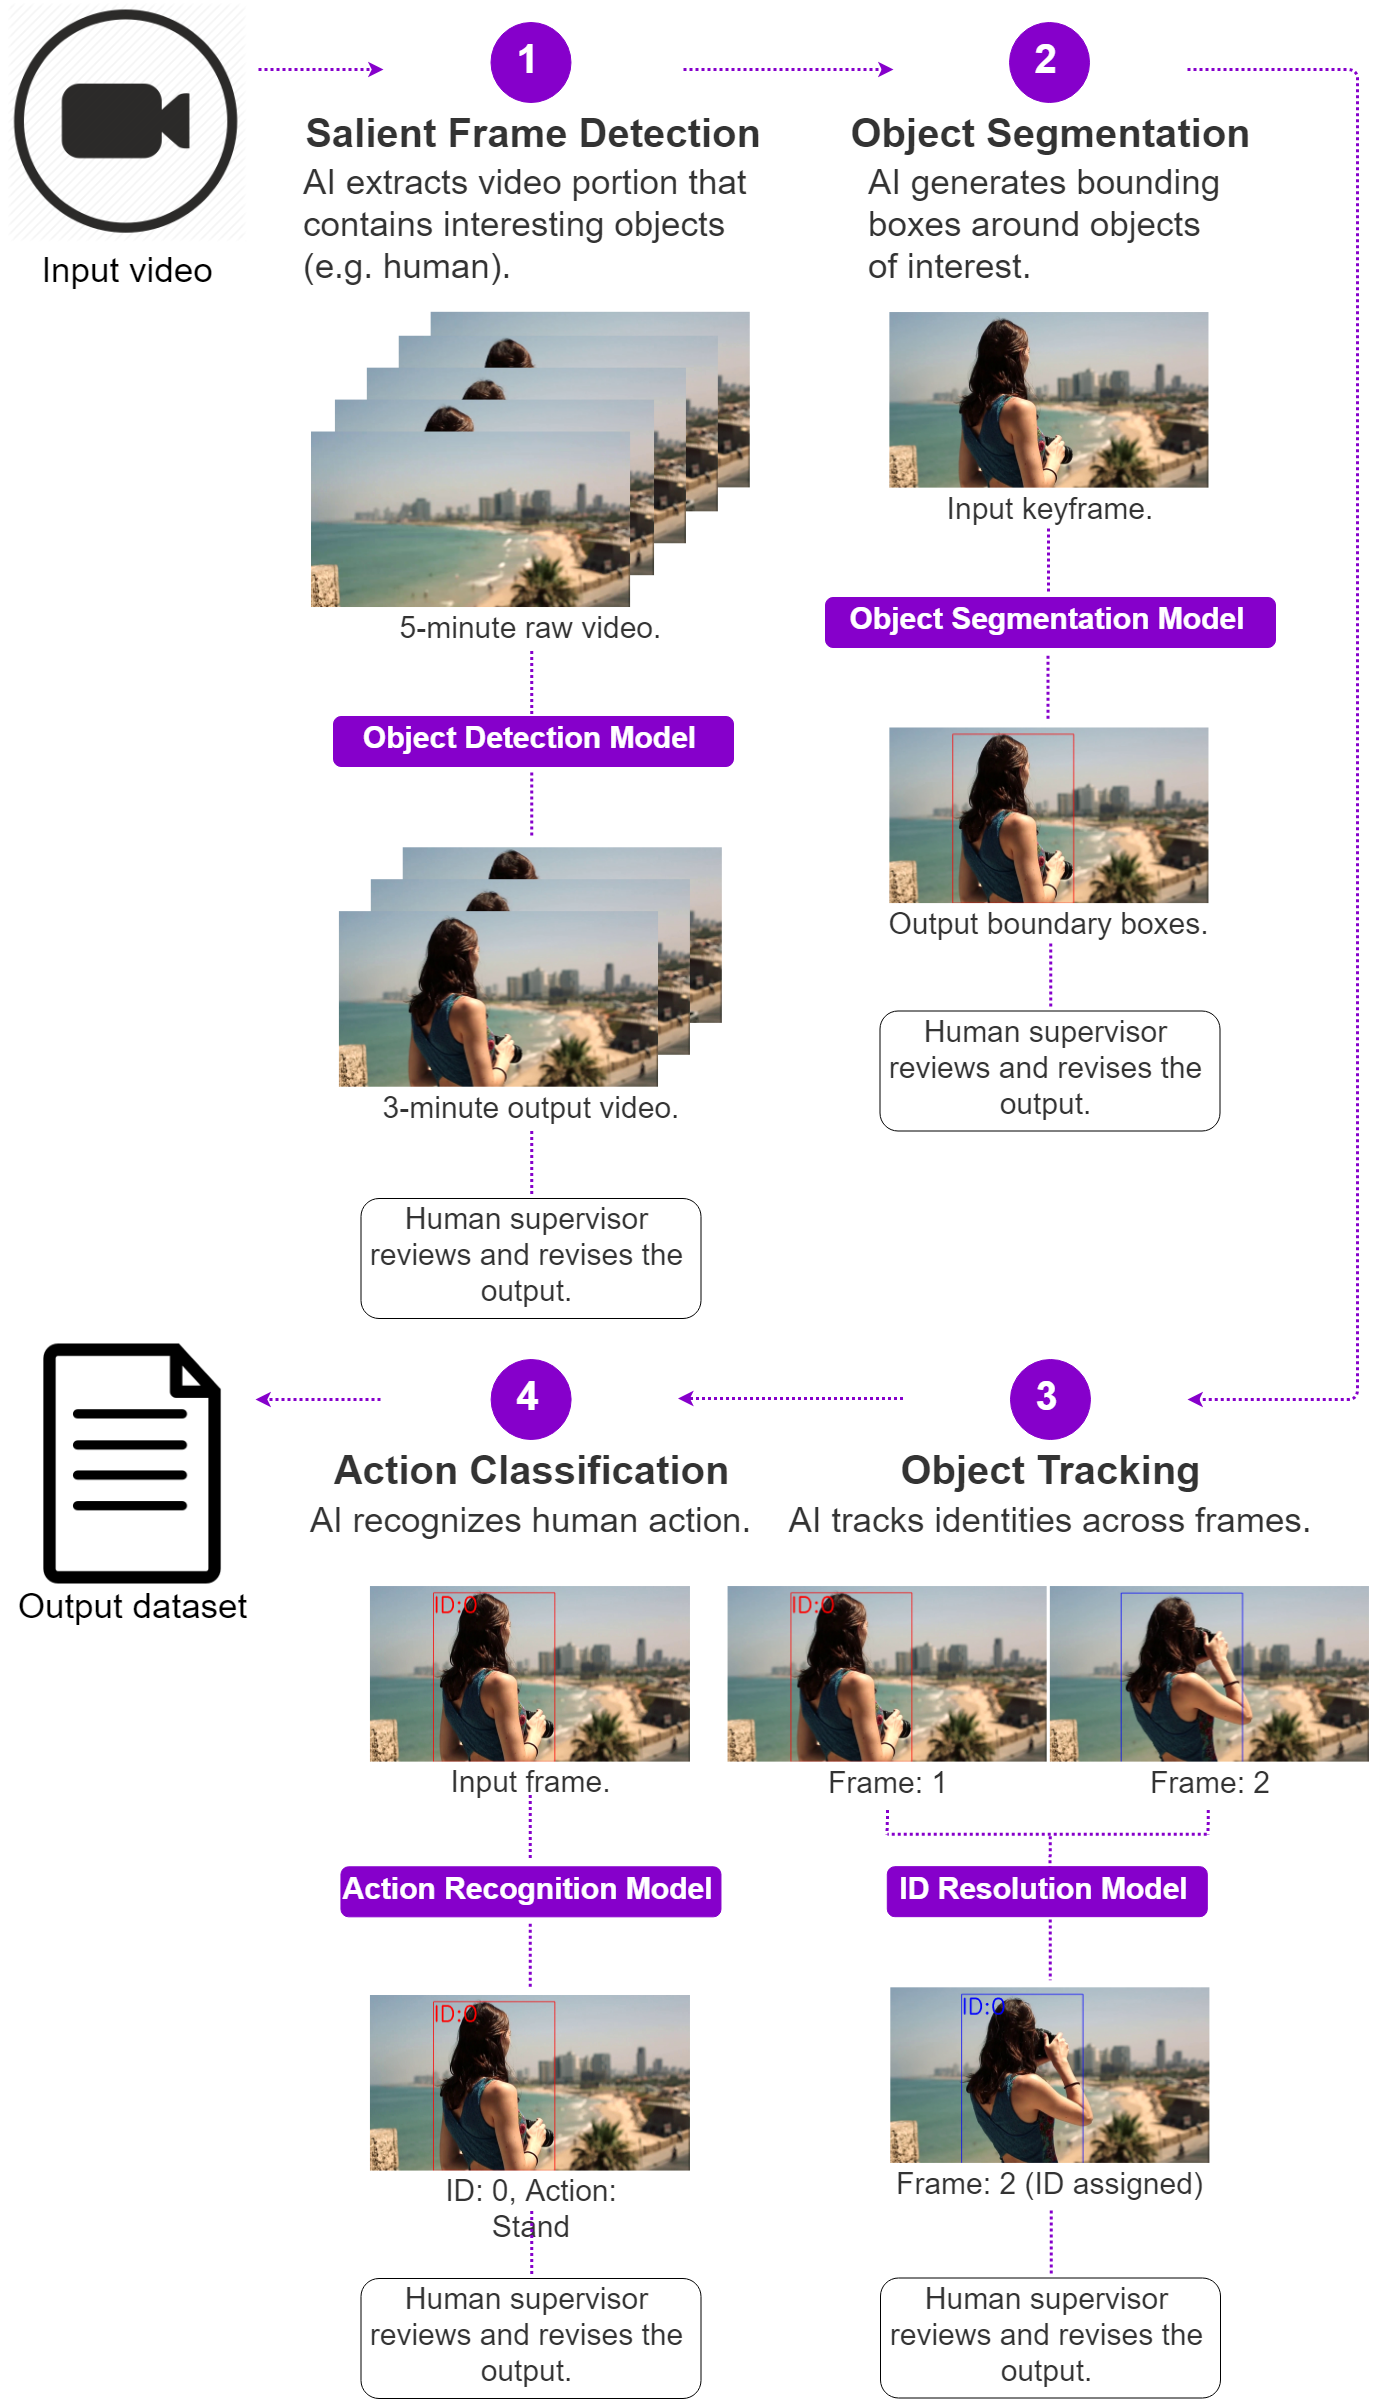
\includegraphics[width=0.95\textwidth, height=1.25\textwidth]{chapter3/images/Overview/HowItWorks.png}
    \caption{ภาพรวมระบบของเครื่องมือสำหรับกำกับข้อมูลด้วยปัญญาประดิษฐ์}
    \label{fig:labeling_overview}
\end{figure}
<<<<<<< HEAD
=======


>>>>>>> 5e103e663a1895ee38cc3363601a5921ca696793
\clearpage

\section{การออกแบบหน้าต่างแอพพลิเคชั่นของเครื่องมือสำหรับกำกับข้อมูลด้วยปัญญาประดิษฐ์}
การออกแบบเครื่องมือสำหรับกำกับข้อมูลด้วยปัญญาประดิษฐ์ ผู้วิจัยได้เลือกใช้ library PyQt และภาษาไพธอนในการพัฒนา
เนื่องจาก PyQt นั้นเป็น library ที่มีผู้พัฒนาใช้กันอย่างแพร่หลาย จึงสะดวกในการศึกษา หาข้อมูลในการสร้างหรือแก้ไข
อีกทั้งยังเป็น library ที่สามารถพัฒนาด้วยภาษาไพธอนได้ และใช้งานง่าย สามารถปรับปรุงแก้ไขได้สะดวก

\subsection{เครื่องมือสำหรับกำกับข้อมูลด้วยปัญญาประดิษฐ์}
เครื่องมือสำหรับกำกับข้อมูลด้วยปัญญาประดิษฐ์ แบ่งการทำงานออกเป็น 4 กระบวนการทำงาน คือ Select, Detect, Track และ Label
เพื่อช่วยแบ่งเบาภาระของผู้พัฒนาในการสร้างชุดข้อมูลสำหรับสร้างโมเดลจากข้อมูลประเภทวิดีโอ โดยกระบวนการ Select
จะต้องสามารถตัดวิดีโอส่วนที่ไม่มีมนุษย์อยู่ออกจากวิดีโอได้ จากนั้นกระบวนการ Detect จะต้องหาตำแหน่งของมนุษย์ภายในวิดีโอได้
แล้วใช้กระบวนการ Track ติดตามการเคลื่อนไหวตำแหน่งต่อไปของมนุษย์ในเฟรมถัดๆไป
และกระบวนการสุดท้าย คือ Label นั้นต้องสามารถทำนายการกระทำพื้นฐานของมนุษย์ได้ เช่น ยืน เดิน นั่ง กินข้าว หรือ นอน เป็นต้น 
โดยทุกส่วนการทำงานมนุษย์ต้องสามารถทำงานร่วมกับปัญญาประดิษฐ์ได้
ดังรูปที่ \ref{fig:labeling_system}

\begin{figure}[!ht]
    \centering
    \includegraphics[width=0.5\textwidth]{chapter3/images/3_6/labelingToolOverview.png}
    \caption{กระบวนการหลักของเครื่องมือสำหรับกำกับข้อมูลด้วยปัญญาประดิษฐ์}
    \label{fig:labeling_system}
\end{figure}
\clearpage

\subsection*{โดยแต่ละกระบวนการจะมีรายละเอียดดังนี้}
\subsection*{หน้าต่าง Select}
กระบวนการ Select จะต้องสามารถรับวิดีโอเข้ามา แล้วตัดวิดีโอในช่วงที่ไม่มนุษย์อยู่ในเฟรมออกได้อัตโนมัติด้วยปัญญาประดิษฐ์
แต่เนื่องจากการประมวลผลทุกเฟรมในวิดีโอนั้นจะทำให้เสียเวลามากเกินไป จึงใช้วิธีการเลือกตัวอย่างเฟรมด้วยอัตราคงที่ (สามารถกำหนดได้)
ซึ่งเรียกเฟรมเหล่านี้ว่า คีย์เฟรม จากนั้นใช้ปัญญาประดิษฐ์ประมวลผลคีย์เฟรม เพื่อลดระยะเวลาในการประมวลผลลง และมนุษย์จะต้องสามารถแก้ไขข้อผิดพลาดของปัญญาประดิษฐ์ได้ เพื่อเพิ่มคุณภาพของชุดข้อมูล จึงออกแบบหน้าต่างได้ดังรูปที่ \ref{fig:SelectDraft}

\begin{figure}[!ht]
    \centering
    \includegraphics[width=1\textwidth]{chapter3/images/3_6/SelectDraft.png}
    \caption{หน้าต่าง Select ของเครื่องมือสำหรับกำกับข้อมูลด้วยปัญญาประดิษฐ์}
    \label{fig:SelectDraft}
\end{figure}
\clearpage
\begin{figure}[!ht]
    \centering
    \includegraphics[width=1\textwidth]{chapter3/images/3_6/SelectDraft_point.png}
    \caption{ตำแหน่งของแต่ละวิดเจ็ตในหน้าต่าง Select}
    \label{fig:SelectDraft_point}
\end{figure}
โดยที่แต่ละวิดเจ็ตตามหมายเลขที่กำหนดตามรูปที่ \ref{fig:SelectDraft_point} มีรายละเอียดดังนี้
\begin{enumerate}
	\setlength\itemsep{-0.25em}
	\item หมายเลข 1 คือปุ่มสำหรับเลือกไฟล์วิดีโอที่ต้องการจากในคอมพิวเตอร์เข้ามาในเครื่องมือกำกับคุณลักษณะด้วยปัญญาประดิษฐ์
    	\item หมายเลข 2 คือปุ่มสำหรับสั่งให้ระบบทำการสุ่มคีย์เฟรมขึ้นมา แล้วใช้ปัญญาประดิษฐ์ประมวลผลเพื่อแยกว่าคีย์เฟรมไหนมีคนอยู่ และคีย์เฟรมไหนไม่มีคนอยู่แบบอัตโนมัติ
    	\item หมายเลข 3 คือแถบเลื่อนเพื่อกำหนดความถี่ในการสุ่มคีย์เฟรม โดยจะมีช่วงอยู่ที่สุ่มหยิบทุกๆ 1 เฟรมต่อวินาที จนถึง อัตราเฟรมต่อวินาทีสูงสุดของวิดีโอที่รับเข้ามา
	\item หมายเลข 4 คือกล่องสำหรับแสดงชื่อวิดีโอที่รับเข้ามาในเครื่องมือกำกับคุณลักษณะด้วยปัญญาประดิษฐ์เพื่อเลือกเข้ามาใช้ในการประมวลผล
	\item หมายเลข 5 คือกล่องสำหรับแสดงว่าคีย์เฟรมใดมีมนุษย์อยู่ในเฟรม โดยที่ผู้ใช้งานสามารถตรวจสอบความถูกต้องและแก้ไขข้อผิดพลาดของปัญญาประดิษฐ์ได้
	\item หมายเลข 6 คือกล่องสำหรับแสดงว่าคีย์เฟรมใดไม่มีมนุษย์อยู่ในเฟรม โดยที่ผู้ใช้งานสามารถตรวจสอบความถูกต้องและแก้ไขข้อผิดพลาดของปัญญาประดิษฐ์ได้
	\item หมายเลข 7 คือหน้าต่างสำหรับแสดงเฟรมที่เลือกจากหมายเลข 5 หมายเลข 6 หรือหมายเลข 8
	\item หมายเลข 8 คือแถบเลื่อนสำหรับเลื่อนดูคีย์เฟรมทั้งหมดที่ระบบสร้างขึ้น
	\item หมายเลข 9 คือปุ่มสำหรับไปกระบวนการต่อไปหลังจากระบบประมวลผลเสร็จแล้ว
\end{enumerate}
\clearpage

\subsection*{หน้าต่าง Detect}
กระบวนการ Delect จะต้องสามารถรับคีย์เฟรมจากกระบวนการ Select มาประมวลผลด้วยปัญญาประดิษฐ์เพื่อหาตำแหน่งของมนุษย์ที่อยู่ในคีย์เฟรม 
แล้วสร้างกรอบสี่เหลี่ยมครอบบริเวณดังกล่าวได้ในแบบอัตโนมัติ เพื่อแบ่งเบาภาระผู้ใช้ในการที่ต้องสร้างกรอบสี่เหลี่ยมครอบตำแหน่งของมนุษย์ด้วยตัวเอง
และผู้ใช้ต้องสามารถสร้างหรือลบกรอบสี่เหลี่ยมได้ด้วยตัวเองสำหรับแก้ไขความผิดพลาดของปัญญาประดิษฐ์ เพื่อเพิ่มคุณภาพของชุดข้อมูล
จึงออกแบบหน้าต่างได้ดังรูปที่ \ref{fig:DetectDraft}
\begin{figure}[!ht]
    \centering
    \includegraphics[width=1\textwidth]{chapter3/images/3_6/DetectDraft.png}
    \caption{หน้าต่าง Detect ของเครื่องมือสำหรับกำกับข้อมูลด้วยปัญญาประดิษฐ์}
    \label{fig:DetectDraft}
\end{figure}
\clearpage
\begin{figure}[!ht]
    \centering
    \includegraphics[width=1\textwidth]{chapter3/images/3_6/DetectDraft_point.png}
    \caption{ตำแหน่งของแต่ละวิดเจ็ตในหน้าต่าง Detect}
    \label{fig:DelectDraft_point}
\end{figure}
โดยที่แต่ละวิดเจ็ตตามหมายเลขที่กำหนดตามรูปที่ \ref{fig:DelectDraft_point} มีรายละเอียดดังนี้
\begin{enumerate}
	\setlength\itemsep{-0.25em}
    \item หมายเลข 1 คือช่องสำหรับกดเพื่อเปลี่ยนระบบจากสร้างกรอบสี่เหลี่ยมในแบบแก้ไขด้วยตนเองเป็นลบกรอบสี่เหลี่ยมแทน
    \item หมายเลข 2 คือช่องสำหรับเลือกว่าจะใช้ระบบการทำงานแบบใด ระหว่างแบบทำงานอัตโนมัติและแบบปรับแก้ไขด้วยตนเอง
    \item หมายเลข 3 คือปุ่มสำหรับสั่งให้ระบบทำการตรวจหาตำแหน่งของมนุษย์ในคีย์เฟรมทั้งหมดแล้วสร้างกรอบสี่เหลี่ยมขึ้นมาครอบบริเวณที่กำหนด
	\item หมายเลข 4 คือกล่องสำหรับแสดงคีย์เฟรมทั้งหมด
	\item หมายเลข 5 คือหน้าต่างสำหรับแสดงเฟรมที่เลือกจากหมายเลข 4 หรือหมายเลข 6
	\item หมายเลข 6 คือแถบเลื่อนสำหรับเลื่อนดูคีย์เฟรมทั้งหมดที่มี เพื่อตรวจสอบความถูกต้องของปัญญาประดิษฐ์
	\item หมายเลข 7 คือปุ่มสำหรับไปกระบวนการต่อไปหลังจากระบบประมวลผลเสร็จแล้ว
\end{enumerate}
\clearpage

\subsection*{หน้าต่าง Track}
เนื่องจากกระบวนการ Detect นั้นจะทำเฉพาะในคีย์เฟรมทำให้ในเฟรมอื่นๆนอกเหนือจากนั้นจะไม่มีกรอบสี่เหลี่ยปรากฎอยู่
ดังนั้นกระบวนการ Track จึงต้องสามารถติดตามการเคลื่อนไหวตำแหน่งต่อไปของมนุษย์ และสร้างกรอบสี่เหลี่ยมขึ้นมาบนเฟรมระหว่างคีย์เฟรมทั้งหมดได้โดยอัตโนมัติ
เพื่อสร้างข้อมูลตำแหน่งของมนุษย์ในเฟรมเหล่านั้น สุดท้ายนี้ผู้ใช้ต้องสามารถสร้างหรือลบกรอบสี่เหลี่ยมได้ด้วยตัวเองสำหรับแก้ไขความผิดพลาดของอัลกอริทึม
จึงออกแบบหน้าต่างได้ดังรูปที่ \ref{fig:TrackDraft}
\begin{figure}[!ht]
    \centering
    \includegraphics[width=1\textwidth]{chapter3/images/3_6/TrackDraft.png}
    \caption{หน้าต่าง Track ของเครื่องมือสำหรับกำกับข้อมูลด้วยปัญญาประดิษฐ์}
    \label{fig:TrackDraft}
\end{figure}
\clearpage
\begin{figure}[!ht]
    \centering
    \includegraphics[width=1\textwidth]{chapter3/images/3_6/TrackDraft_point.png}
    \caption{ตำแหน่งของแต่ละวิดเจ็ตในหน้าต่าง Track}
    \label{fig:TrackDraft_point}
\end{figure}
โดยที่แต่ละวิดเจ็ตตามหมายเลขที่กำหนดตามรูปที่ \ref{fig:TrackDraft_point} มีรายละเอียดดังนี้
\begin{enumerate}
	\setlength\itemsep{-0.25em}
    \item หมายเลข 1 คือช่องสำหรับกดเพื่อเปลี่ยนระบบจากสร้างกรอบสี่เหลี่ยมในแบบแก้ไขด้วยตนเองเป็นลบกรอบสี่เหลี่ยมแทน
    \item หมายเลข 2 คือช่องสำหรับเลือกว่าจะใช้ระบบแบบใด ระหว่างแบบอัตโนมัติและแบบแก้ไขด้วยตนเอง
    \item หมายเลข 3 คือปุ่มสำหรับสั่งให้ระบบทำการตรวจหาตำแหน่งของมนุษย์ในเฟรมระหว่างคีย์เฟรมทั้งหมดแล้วสร้างกรอบสี่เหลี่ยมขึ้นมาครอบบริเวณที่กำหนด
	\item หมายเลข 4 คือกล่องสำหรับแสดงกรอบสี่เหลี่ยมทั้งหมดที่อยู่ในเฟรม
	\item หมายเลข 5 คือหน้าต่างสำหรับแสดงเฟรมที่เลือกจากหมายเลข 6
	\item หมายเลข 6 คือแถบเลื่อนสำหรับเลื่อนดูเฟรมทั้งหมดที่มี เพื่อตรวจสอบความถูกต้องของอัลกอริทึม
	\item หมายเลข 7 คือปุ่มสำหรับไปกระบวนการต่อไปหลังจากระบบประมวลผลเสร็จแล้ว
\end{enumerate}
\clearpage

\subsection*{หน้าต่าง Label}
กระบวนการ Label นั้นต้องสามารถทำนายว่าการกระทำของมนุษย์ที่อยู่ในแต่ละเฟรมว่าคืออะไรได้โดยอัตโนมัติด้วยปัญญาประดิษฐ์
และผู้ใช้จะต้องสามารถแก้ไขข้อผิดพลาดของปัญญาประดิษฐ์ได้หากมีการทำนายที่ผิดพลาดเกิดขึ้น
หรือถ้าหากผู้ใช้ต้องการเพิ่มการกระทำที่ไม่ได้มีอยู่ในชุดการกระทำพื้นฐานที่มีอยู่แล้วของปัญญาประดิษฐ์ ผู้ใช้ก็สามารถเพิ่มการกระทำนั้นเข้ามาได้
จึงออกแบบหน้าต่างได้ดังรูปที่ \ref{fig:ActionLabelDraft}
\begin{figure}[!ht]
    \centering
    \includegraphics[width=1\textwidth]{chapter3/images/3_6/ActionLabelDraft.png}
    \caption{หน้าต่าง Label ของเครื่องมือสำหรับกำกับข้อมูลด้วยปัญญาประดิษฐ์}
    \label{fig:ActionLabelDraft}
\end{figure}
\clearpage
\begin{figure}[!ht]
    \centering
    \includegraphics[width=1\textwidth]{chapter3/images/3_6/ActionLabelDraft_point.png}
    \caption{ตำแหน่งของแต่ละวิดเจ็ตในหน้าต่าง Label}
    \label{fig:ActiobLabelDraft_point}
\end{figure}
โดยที่แต่ละวิดเจ็ตตามหมายเลขที่กำหนดตามรูปที่ \ref{fig:TrackDraft_point} มีรายละเอียดดังนี้
\begin{enumerate}
	\setlength\itemsep{-0.25em}
    \item หมายเลข 1 คือช่องสำหรับเลือกว่าจะใช้ระบบแบบใด ระหว่างแบบอัตโนมัติและแบบแก้ไขด้วยตนเอง
    \item หมายเลข 2 คือปุ่มสำหรับสั่งให้ระบบทำนายการกระทำของมนุษย์ในทุกๆเฟรม
    \item หมายเลข 3 คือกล่องสำหรับแสดงกรอบสี่เหลี่ยมทั้งหมดที่อยู่ในเฟรมที่เลือก
	\item หมายเลข 4 คือกล่องสำหรับแสดงการกระทำของมนุษย์แต่ละคนที่อยู่ในเฟรมที่เลือก โดยจะเรียงลำดับคู่กับกรอบสี่เหลี่ยมที่อยู่ในช่องหมายเลข 3
    \item หมายเลข 5 คือกล่องสำหรับแสดงชุดการกระทำที่ปัญญาประดิษฐ์มีอยู่แล้ว ซึ่งในการทำงานแบบแก้ไขด้วยตนเองนั้น จะสามารถค้นหาการกระทำที่มีอยู่แล้วได้ 
    และหากคำที่ใส่เข้ามานั้นไม่มีอยู่ในชุดการกระทำก็จะเป็นการเพิ่มการกระทำนั้นเข้ามาแทน
	\item หมายเลข 6 คือหน้าต่างสำหรับแสดงเฟรมที่เลือกจากหมายเลข 7
	\item หมายเลข 7 คือแถบเลื่อนสำหรับเลื่อนดูเฟรมทั้งหมดที่มี เพื่อตรวจสอบความถูกต้องของปัญญาประดิษฐ์
	\item หมายเลข 8 คือปุ่มสำหรับสร้างไฟล์ xml ของทุกๆเฟรมสำหรับใช้ในการสร้างโมเดลโดยรายละเอียดข้อมูลภายในไฟล์ xml จะอยู่ในหัวข้อ \ref{sec:XMLInfo}
\end{enumerate}
\clearpage

\subsection*{รายละเอียดข้อมูลภายในไฟล์ xml}
\label{sec:XMLInfo}
ไฟล์ xml นั้นเป็นรูปแบบที่นิยมใช้ในการเก็บข้อมูลสำหรับการสร้างโมเดลประเภทตรวจจับวัตถุ
โดยจะเก็บข้อมูลในรูปแบบของ PASCAL VOC ที่นิยมใช้ในการสร้างโมเดลด้วย Tensorflow โดยภายในไฟล์จะมีข้อมูลดังรูปที่ \ref{fig:XMLFormat}
\begin{figure}[!ht]
    \centering
    \includegraphics[width=1\textwidth]{chapter3/images/3_6/XMLFormat.png}
    \caption{ตัวอย่างข้อมูลภายในไฟล์ xml}
    \label{fig:XMLFormat}
\end{figure}
โดยข้อมูลส่วนสำคัญของรูปแบบนี้นั้นจะถูกใส่หมายเลขกำกับไว้ซึ่งแต่ละหมายเลขนั้นหมายถึง
\begin{enumerate}
	\setlength\itemsep{-0.25em}
    \item หมายเลข 1 คือชื่อโฟลเดอร์ที่เก็บไฟล์รูปภาพที่เกี่ยวข้องกับไฟล์ xml นี้อยู่
    \item หมายเลข 2 คือชื่อไฟล์ที่เกี่ยวข้องกับไฟล์ xml นี้
    \item หมายเลข 3 คือเส้นทางในคอมพิวเตอร์ (directory path) ของไฟล์รูปภาพที่เกี่ยวข้องกับไฟล์ xml นี้
    \item หมายเลข 4 คือขนาดและมิติของรูปภาพ ซึ่งจะประกอบด้วยความกว้าง (width) ความยาว (height) และจำนวนช่องสี (depth) 
    โดยที่จำนวนช่องสีที่มีความลึก 3 มักจะหมายถึงภาพสี RGB และจำนวนช่องสีที่มีความลึก 2 จะหมายถึงภาพขาวดำ (gray scale)
	\item หมายเลข 5 คือ label ของวัตถุหรืออย่างอื่น ที่อยู่ในกรอบสี่เหลี่ยมที่ถูกกำหนดไว้ในส่วนของหมายเลข 6
	\item หมายเลข 6 คือ กรอบสี่เหลี่ยมที่ครอบวัตถุที่สนใจ เช่นมนุษย์ เป็นต้น
\end{enumerate}
\clearpage

\section{การออกแบบระบบวิเคราะห์การกระทำของมนุษย์}
<<<<<<< HEAD
\subsection{ทดสอบประสิทธิ์ภาพการทำงานของระบบทำนายตำแหน่งต่อไปของวัตถุในวิดีโอ}
\subsection*{สิ่งที่ใช้ในการวัดผล}
	\begin{enumerate}
		\setlength\itemsep{-0.25em}
		\item ความเร็วในการทำนายต่อวิดีโอ (วินาที)
		\item ความแม่นยำ โดยคำนึงถึง IoU
	\end{enumerate}
\subsection*{วัตถุประสงค์}
ผู้วิจัยมีความต้องการทดสอบความแม่นยำและความเร็วของการใช้โมเดลปัญญาประดิษฐ์สำหรับตรวจจับวัตถุและสร้างกรอบสี่เหลี่ยมทุกๆ N เฟรม 
และใช้ระบบติดตามการเคลื่อนไหวตำแหน่งต่อไปของวัตถุในการสร้างกรอบสี่เหลี่ยมในเฟรมระหว่างนั้น ว่าด้วยความเร็วที่เพิ่มขึ้นมานั้นทำให้ความแม่นยำลดลงไปเท่าไหร่
\subsection*{ตัวแปรควบคุม}
	\begin{enumerate}
		\setlength\itemsep{-0.25em}
		\item วิดีโอสาธารณะที่ไม่ติดลิขสิทธิ์ ความยาวประมาณ 10 - 30 วินาที หนึ่งวิดีโอ
		\item ใช้โมเดลปัญญาประดิษฐ์สำหรับตรวจจับตำแหน่งวัตถุ ResNet50 ในการสร้างชุดข้อมูลที่มีการกำกับตำแหน่งวัตถุไว้ และใช้มนุษย์ในการตรวจสอบความถูกต้อง
		เพื่อใช้เป็นชุดข้อมูลที่มีค่ากำกับตำแหน่งเพื่อใช้สำหรับวัดผล
		\item โมเดลปัญญาประดิษฐ์สำหรับตรวจจับตำแหน่งที่ใช้ในการเปรียบเทียบ: YOLO-v3 spp
		\item อัลกอริทึมสำหรับระบบการติดตามการเคลื่อนไหวตำแหน่งต่อไปของวัตถุ: Dlib
		\item IoU: มีส่วนที่ทับกันมากกว่า 80\% ขึ้นไปจึงจะนับว่าผลการทำนายถูกต้อง
	\end{enumerate}
\subsection*{วิธีการทดลอง}
	\begin{enumerate}
		\setlength\itemsep{-0.25em}
		\item ใช้โมเดลปัญญาประดิษฐ์ YOLO-v3 spp ประมวลผลทุกเฟรมในวิดีโอ และเปรียบเทียบผลลัพธ์กับชุดข้อมูลที่มีค่ากำกับตำแหน่งวัตถุไว้แล้ว เพื่อคำนวณหาความแม่นยำ
		\item ใช้โมเดลปัญญาประดิษฐ์ YOLO-v3 spp ประมวลผลทุกๆ N เฟรมในวิดีโอ แล้วใช้ระบบติดตามการเคลื่อนไหวตำแหน่งต่อไปของวัตถุในการสร้างกรอบสี่เหลี่ยมในเฟรมระหว่างนั้น 
		และเปรียบเทียบผลลัพธ์กับชุดข้อมูลที่มีค่ากำกับตำแหน่งวัตถุไว้แล้ว เพื่อคำนวณหาความแม่นยำ โดยที่ค่า N จะเท่ากับ 10 20 และ 25
		\item เปรียบเทียบความเร็วในการประมวลผล และความแม่นยำ
\end{enumerate}
\clearpage

\subsection{ทดสอบประสิทธิ์ภาพการทำงานของโมเดลที่เคยถูกเทรนด์ผ่าน AVA เทียบผลลัพธ์กับแหล่งอ้างอิง}
\subsection*{สิ่งที่ใช้ในการวัดผล}
	\begin{enumerate}
		\setlength\itemsep{-0.25em}
		\item ความเร็วในการทำนายต่อรูปภาพ (มิลลิวินาที)
		\item ความแม่นยำ (PASCAL mAP)
	\end{enumerate}
\subsection*{สมมติฐาน}
ผู้วิจัยได้ตั้งสมมติฐานว่า ผลลัพธ์ของการทดลองจะมีความแม่นยำเทียบเท่ากับผลลัพธ์จากแหล่งที่มา และความเร็วต่อรูปภาพจะมีความเร็วมากกว่ากว่าผลลัพธ์จากแหล่งที่มา 
เนื่องจากแหล่งที่มาของข้อมูลได้ทำการทดสอบโดยใช้กราฟิกการ์ดรุ่น Nvidia GeForce GTX TITAN X ซึ่งเป็นกราฟิกการ์ดที่มีประสิทธิภาพการทำงานดีน้อยกว่ากราฟิกการ์ดของผู้วิจัย
\subsection*{ตัวแปรควบคุม}
	\begin{enumerate}
		\setlength\itemsep{-0.25em}
		\item ชุดข้อมูล : The validation split of AVA v2.1
		\item โมเดลปัญญาประดิษฐ์ : Faster RCNN ResNet101 AVA v2.1
	\end{enumerate}
\subsection*{วิธีการทดลอง}
	\begin{enumerate}
		\setlength\itemsep{-0.25em}
		\item ดาวน์โหลดชุดข้อมูล The validation split of AVA v2.1
		\item แบ่งชุดข้อมูลออกเป็น ชุดข้อมูลสำหรับทดสอบ และชุดข้อมูลที่มีคำกำกับเพื่อเป็นคำตอบ
			\begin{enumerate}
				\setlength\itemsep{-0.25em}
				\item ชุดข้อมูลสำหรับทดสอบ ประกอบด้วย : ชื่อของวิดีโอ
				\item ชุดข้อมูลที่มีคำกำกับเพื่อเป็นคำตอบ ประกอบด้วย : ชื่อของวิดีโอ เฟรม ตำแหน่งของกรอบสี่เหลี่ยม และรหัสของการกระทำ
			\end{enumerate}
		\item เรียกชื่อของวิดีโอจากชุดข้อมูลทดสอบ และนำโมเดลปัญญาประดิษฐ์ทำนายผลลัพธ์ จากนั้นเก็บผลลัพธ์เป็นชุดข้อมูลผลลัพธ์จากการทำนาย
			\begin{enumerate}
				\setlength\itemsep{-0.25em}
				\item ชุดข้อมูลผลลัพธ์จากการทำนาย ประกอบด้วย : ชื่อของวิดีโอ เฟรม ตำแหน่งของกรอบสี่เหลี่ยม รหัสของการกระทำ และความมั่นใจ
			\end{enumerate}
		\item ประเมินผลการทำงานโดยเทียบระหว่างชุดผลลัพธ์จากการทำนาย และชุดข้อมูลที่มีคำกำกับเพื่อเป็นคำตอบ
		\item เปรียบเทียบผลลัพธ์จากแหล่งที่มา
\end{enumerate}
\clearpage
\subsection{ทดสอบประสิทธิภาพการทำงานของโมเดลปัญญาประดิษฐ์ Faster RCNN ResNet101 ที่เคยถูกสร้างด้วยชุดข้อมูลของ AVA และใช้ชุดข้อมูลที่ผู้วิจัยสร้างขึ้นในการทดสอบและเทียบผลลัพธ์กับแหล่งอ้างอิง}
\subsection*{สิ่งที่ใช้ในการวัดผล}
	\begin{enumerate}
		\setlength\itemsep{-0.25em}
		\item ความในการทำนายเร็วต่อรูปภาพ (มิลลิวินาที)
		\item ความแม่นยำ (PASCAL mAP)
	\end{enumerate}
\subsection*{สมมติฐาน}ผู้วิจัยได้ตั้งสมมติฐานว่าผลลัพธ์ของการทดลองจะมีความแม่นยำต่ำลงเมื่อเทียบกับความแม่นยำของการทดลองที่ผ่านมา เนื่องจากชุดข้อมูลที่ผู้วิจัยสร้างขึ้น ได้มีการตัดหมวดหมู่บางอย่างออกไป 
ทำให้โมเดลปัญญาประดิษฐ์ที่ถูกสร้างด้วย AVA มีหมวดหมู่ของการกระทำไม่ตรงกับชุดข้อมูลที่ผู้วิจัยสร้างขึ้น ซึ่งมีผลทำให้ความแม่นยำลดลง ในส่วนของความเร็วต่อรูปภาพจะมีความเร็วมากกว่าผลลัพธ์จากแหล่งที่มา เนื่องจาก แหล่งที่มาของข้อมูลได้ทำการทดสอบโดยใช้กราฟิกการ์ดรุ่น Nvidia GeForce GTX TITAN X card ซึ่งเป็นกราฟิกการ์ดที่มีประสิทธิภาพการทำงานดีน้อยกว่า กราฟิกการ์ดของผู้วิจัย
\subsection*{ตัวแปรควบคุม}
	\begin{enumerate}
		\setlength\itemsep{-0.25em}
		\item ชุดข้อมูล : ชุดข้อมูลที่ผู้วิจัยสร้างด้วยเครื่องมือกำกับคุณลักษณะ
		\item โมเดลปัญญาประดิษฐ์ : Faster RCNN ResNet101 AVA v2.1
	\end{enumerate}
\subsection*{วิธีการทดลอง}
	\begin{enumerate}
		\setlength\itemsep{-0.25em}
		\item แบ่งชุดข้อมูลออกเป็น ชุดข้อมูลสำหรับทดสอบ และชุดข้อมูลที่มีคำกำกับเพื่อเป็นคำตอบ
			\begin{enumerate}
				\setlength\itemsep{-0.25em}
				\item ชุดข้อมูลสำหรับทดสอบ ประกอบด้วย : ชื่อของวิดีโอ
				\item ชุดข้อมูลที่มีคำกำกับเพื่อเป็นคำตอบ ประกอบด้วย : ชื่อของวิดีโอ เฟรม ตำแหน่งของกรอบสี่เหลี่ยม และรหัสของการกระทำ
			\end{enumerate}
		\item เรียกชื่อของวิดีโอจากชุดข้อมูลทดสอบ และนำโมเดลปัญญาประดิษฐ์ทำนายผลลัพธ์ จากนั้นเก็บผลลัพธ์เป็นชุดข้อมูลผลลัพธ์จากการทำนาย
			\begin{enumerate}
				\setlength\itemsep{-0.25em}
				\item ชุดข้อมูลผลลัพธ์จากการทำนาย ประกอบด้วย : ชื่อของวิดีโอ เฟรม ตำแหน่งของกรอบสี่เหลี่ยม รหัสของการกระทำ และความมั่นใจ
			\end{enumerate}
		\item ประเมินผลการทำงานโดยเทียบระหว่างชุดผลลัพธ์จากการทำนาย และชุดข้อมูลที่มีคำกำกับเพื่อเป็นคำตอบ	
		\item เปรียบเทียบผลลัพธ์กับผลการทดลองที่ผ่านมา
\end{enumerate}
\clearpage
\subsection{ทดสอบประสิทธิภาพการทำงานของโมเดลปัญญาประดิษฐ์ ResNet50 ที่ถูกสร้างด้วยชุดข้อมูลที่ผู้วิจัยสร้างขึ้น และใช้ชุดข้อมูลที่ผู้วิจัยสร้างขึ้นในการทดสอบและเทียบผลลัพธ์กับแหล่งอ้างอิง}
\subsection*{สิ่งที่ใช้ในการวัดผล}
	\begin{enumerate}
		\setlength\itemsep{-0.25em}
		\item ความเร็วในการทำนายต่อรูปภาพ (มิลลิวินาที)
		\item ความแม่นยำ (PASCAL mAP)
	\end{enumerate}
\subsection*{สมมติฐาน}ผู้วิจัยได้ตั้งสมมติฐานว่าผลลัพธ์ของการทดลองจะมีความแม่นยำสูงขึ้นเมื่อเทียบกับความแม่นยำของการทดลองที่ผ่านมา เนื่องจากโมเดลปัญญาประดิษฐ์ในการทดลองนี้ 
เป็นโมเดลปัญญาประดิษฐ์ที่ผู้วิจัยได้สร้างขึ้น ซึ่งจะมีหมวดหมู่ของการกระทำของโมเดลปัญญาประดิษฐ์และชุดข้อมูลทดสอบตรงกัน ในส่วนของความเร็วต่อรูปภาพจะมีความเร็วมากกว่าผลลัพธ์จากแหล่งที่มา 
เนื่องจากแหล่งที่มาของข้อมูลได้ทำการทดสอบโดยใช้กราฟิกการ์ดรุ่น Nvidia GeForce GTX TITAN X ซึ่งเป็นกราฟิกการ์ดที่มีประสิทธิภาพการทำงานดีน้อยกว่ากราฟิกการ์ดของผู้วิจัย
\subsection*{ตัวแปรควบคุม}
	\begin{enumerate}
		\setlength\itemsep{-0.25em}
		\item ชุดข้อมูล : ชุดข้อมูลที่ผู้วิจัยสร้างด้วยเครื่องมือกำกับคุณลักษณะ
		\item โมเดลปัญญาประดิษฐ์ : โมเดลปัญญาประดิษฐ์ที่ผู้วิจัยสร้างขึ้น
	\end{enumerate}
\subsection*{วิธีการทดลอง}
	\begin{enumerate}
		\setlength\itemsep{-0.25em}
		\item แบ่งชุดข้อมูลออกเป็น ชุดข้อมูลที่ใช้สำหรับการสร้างโมเดลปัญญาประดิษฐ์ และชุดข้อมูลสำหรับทดสอบที่มีคำกำกับเพื่อเป็นคำตอบ โดยคำกำกับจะประกอบไปด้วย : ชื่อของวิดีโอ เฟรม ตำแหน่งของกรอบสี่เหลี่ยม และรหัสของการกระทำ
		\item ทำการสร้างโมเดลปัญญาประดิษฐ์ด้วยชุดข้อมูลที่เตรียมไว้ และนำโมเดลปัญญาประดิษฐ์ทำนายผลลัพธ์กับชุดข้อมูลทดสอบ จากนั้นเก็บผลลัพธ์จากการทำนาย  ประกอบด้วย : ชื่อของวิดีโอ เฟรม ตำแหน่งของกรอบสี่เหลี่ยม รหัสของการกระทำ และค่าความมั่นใจ โดยรายละเอียดของชุดข้อมูลทดสอบมีดังนี้
	\begin{table}[!ht]
                \centering
                \begin{tabular}{|c|c|}
                    \hline
                    Label & Test set\\
                    \hline
                    Play phone  & 3,888 \\
                    Eat  & 3,000\\
                    Sit   & 5,591\\
                    Sleep  & 2,458\\
                    Stand  & 1,402\\
                    Walk  & 2,162\\
                    \hline
                \end{tabular}
                \caption{ตารางแสดงจำนวนภาพที่ใช้ในการทดลองนี้}
                \label{tab: ResNet50_datasetInfo}
	\end{table}
		\item มีการปรับเปลี่ยนการเตรียมข้อมูลเช่นการใช้ pretrain โมเดลหรือการปรับขนาดสเกลของชุดข้อมูลที่ใช้ในการสร้างโมเดลปัญญาประดิษฐ์
		\item เปรียบเทียบผลลัพธ์ของโมเดลปัญญาประดิษฐ์ เพื่อเปรียบเทียบประสิทธิภาพ
\end{enumerate}






=======
\subsection{ทดสอบประสิทธิ์ภาพการทำงานของโมเดลปัญญาประดิษฐ์สำหรับการทำการตรวจจับภาพบุคคล}
\subsection*{สิ่งที่ใช้ในการวัดผล}
	\begin{enumerate}
		\item ความเร็วต่อรูปภาพ (วินาที)
		\item ความแม่นยำของกรอบสี่เหลี่ยม (IOU)
	\end{enumerate}
\subsection*{สมมุติฐาน :}
\subsection*{ตัวแปร}
	\begin{enumerate}
		\item โมเดลปัญญาประดิษฐ์ ซึ่งได้แก่
		\begin{enumerate}
			\item Tiny YOLO
			\item YOLOv3-tiny
			\item SSD300	
			\item YOLOv3-320
			\item YOLOv2 608x608
		\end{enumerate}
	\end{enumerate}
\subsection*{ตัวแปรควบคุม}
	\begin{enumerate}
		\item ชุดข้อมูล : The validation split of AVA v2.1
	\end{enumerate}
\subsection*{วิธีการทดลอง}
	\begin{enumerate}
		\item ดาว์นโหลดชุดข้อมูล The validation split of AVA v2.1
		\item แบ่งชุดข้อมูลออกเป็น ชุดข้อมูลสำหรับทดสอบ และ ชุดข้อมูลที่มีคำตอบ
			\begin{enumerate}
				\item ชุดข้อมูลสำหรับทดสอบ ประกอบด้วย : ชื่อของวิดีโอ,เฟรม
				\item ชุดข้อมูลที่มีคำตอบ ประกอบด้วย : ชื่อของวิดีโอ,เฟรม,ตำแหน่งของกรอบสี่เหลี่ยม
			\end{enumerate}
		\item เรียกชื่อและเฟรมของวิดีโอจากชุดข้อมูลทดสอบ และนำโมเดลปัญญาประดิษฐ์ทำนายผลลัพธ์ จากนั้นเก็บผลลัพธ์เป็น ชุดข้อมูลผลลัพธ์จากการทำนาย
			\begin{enumerate}
				\item ชุดข้อมูลผลลัพธ์จากการทำนาย ประกอบด้วย : ชื่อของวิดีโอ,เฟรม,ตำแหน่งของกรอบสี่เหลี่ยม
			\end{enumerate}
		\item ประเมินผลการทำงานโดยเทียบระหว่างชุดผลลัพธ์จากการทำนาย และ ชุดข้อมูลที่มีคำตอบ ผ่านฟังก์ชั่นคำนวณค่า IOU		
		\item เปรียบเทียบผลลัพธ์จากแหล่งที่มา
\end{enumerate}



\subsection{ทดสอบประสิทธิ์ภาพการทำงานของโมเดลปัญญาประดิษฐ์ที่เคยถูกเทรนด์ผ่าน AVA เทียบผลลัพธ์กับแหล่งอ้างอิง}
\subsection*{สิ่งที่ใช้ในการวัดผล}
	\begin{enumerate}
		\setlength\itemsep{-0.25em}
		\item ความเร็วในการทำนายต่อรูปภาพ (มิลลิวินาที)
		\item ความแม่นยำ (PASCAL mAP)
	\end{enumerate}
\subsection*{สมมติฐาน}
ผู้วิจัยได้ตั้งสมมติฐานว่า ผลลัพธ์ของการทดลองจะมีความแม่นยำเทียบเท่ากับผลลัพธ์จากแหล่งที่มา และความเร็วต่อรูปภาพจะมีความเร็วมากกว่ากว่าผลลัพธ์จากแหล่งที่มา 
เนื่องจากแหล่งที่มาของข้อมูลได้ทำการทดสอบโดยใช้กราฟิกการ์ดรุ่น Nvidia GeForce GTX TITAN X ซึ่งเป็นกราฟิกการ์ดที่มีประสิทธิภาพการทำงานดีน้อยกว่ากราฟิกการ์ดของผู้วิจัย
\subsection*{ตัวแปรควบคุม}
	\begin{enumerate}
		\setlength\itemsep{-0.25em}
		\item ชุดข้อมูล : The validation split of AVA v2.1
		\item โมเดลปัญญาประดิษฐ์ : Faster RCNN ResNet101 AVA v2.1
	\end{enumerate}
\subsection*{วิธีการทดลอง}
	\begin{enumerate}
		\setlength\itemsep{-0.25em}
		\item ดาวน์โหลดชุดข้อมูล The validation split of AVA v2.1
		\item แบ่งชุดข้อมูลออกเป็น ชุดข้อมูลสำหรับทดสอบ และชุดข้อมูลที่มีคำกำกับเพื่อเป็นคำตอบ
			\begin{enumerate}
				\setlength\itemsep{-0.25em}
				\item ชุดข้อมูลสำหรับทดสอบ ประกอบด้วย : ชื่อของวิดีโอ
				\item ชุดข้อมูลที่มีคำกำกับเพื่อเป็นคำตอบ ประกอบด้วย : ชื่อของวิดีโอ เฟรม ตำแหน่งของกรอบสี่เหลี่ยม และรหัสของการกระทำ
			\end{enumerate}
		\item เรียกชื่อของวิดีโอจากชุดข้อมูลทดสอบ และนำโมเดลปัญญาประดิษฐ์ทำนายผลลัพธ์ จากนั้นเก็บผลลัพธ์เป็นชุดข้อมูลผลลัพธ์จากการทำนาย
			\begin{enumerate}
				\setlength\itemsep{-0.25em}
				\item ชุดข้อมูลผลลัพธ์จากการทำนาย ประกอบด้วย : ชื่อของวิดีโอ เฟรม ตำแหน่งของกรอบสี่เหลี่ยม รหัสของการกระทำ และความมั่นใจ
			\end{enumerate}
		\item ประเมินผลการทำงานโดยเทียบระหว่างชุดผลลัพธ์จากการทำนาย และชุดข้อมูลที่มีคำกำกับเพื่อเป็นคำตอบ
		\item เปรียบเทียบผลลัพธ์จากแหล่งที่มา
\end{enumerate}
\clearpage
\subsection{ทดสอบประสิทธิภาพการทำงานของโมเดลปัญญาประดิษฐ์ Faster RCNN ResNet101 ที่เคยถูกสร้างด้วยชุดข้อมูลของ AVA และใช้ชุดข้อมูลที่ผู้วิจัยสร้างขึ้นในการทดสอบและเทียบผลลัพธ์กับแหล่งอ้างอิง}
\subsection*{สิ่งที่ใช้ในการวัดผล}
	\begin{enumerate}
		\setlength\itemsep{-0.25em}
		\item ความในการทำนายเร็วต่อรูปภาพ (มิลลิวินาที)
		\item ความแม่นยำ (PASCAL mAP)
	\end{enumerate}
\subsection*{สมมติฐาน}ผู้วิจัยได้ตั้งสมมติฐานว่าผลลัพธ์ของการทดลองจะมีความแม่นยำต่ำลงเมื่อเทียบกับความแม่นยำของการทดลองที่ผ่านมา เนื่องจากชุดข้อมูลที่ผู้วิจัยสร้างขึ้น ได้มีการตัดหมวดหมู่บางอย่างออกไป 
ทำให้โมเดลปัญญาประดิษฐ์ที่ถูกสร้างด้วย AVA มีหมวดหมู่ของการกระทำไม่ตรงกับชุดข้อมูลที่ผู้วิจัยสร้างขึ้น ซึ่งมีผลทำให้ความแม่นยำลดลง ในส่วนของความเร็วต่อรูปภาพจะมีความเร็วมากกว่าผลลัพธ์จากแหล่งที่มา เนื่องจาก แหล่งที่มาของข้อมูลได้ทำการทดสอบโดยใช้กราฟิกการ์ดรุ่น Nvidia GeForce GTX TITAN X card ซึ่งเป็นกราฟิกการ์ดที่มีประสิทธิภาพการทำงานดีน้อยกว่า กราฟิกการ์ดของผู้วิจัย
\subsection*{ตัวแปรควบคุม}
	\begin{enumerate}
		\setlength\itemsep{-0.25em}
		\item ชุดข้อมูล : ชุดข้อมูลที่ผู้วิจัยสร้างด้วยเครื่องมือกำกับคุณลักษณะ
		\item โมเดลปัญญาประดิษฐ์ : Faster RCNN ResNet101 AVA v2.1
	\end{enumerate}
\subsection*{วิธีการทดลอง}
	\begin{enumerate}
		\setlength\itemsep{-0.25em}
		\item แบ่งชุดข้อมูลออกเป็น ชุดข้อมูลสำหรับทดสอบ และชุดข้อมูลที่มีคำกำกับเพื่อเป็นคำตอบ
			\begin{enumerate}
				\setlength\itemsep{-0.25em}
				\item ชุดข้อมูลสำหรับทดสอบ ประกอบด้วย : ชื่อของวิดีโอ
				\item ชุดข้อมูลที่มีคำกำกับเพื่อเป็นคำตอบ ประกอบด้วย : ชื่อของวิดีโอ เฟรม ตำแหน่งของกรอบสี่เหลี่ยม และรหัสของการกระทำ
			\end{enumerate}
		\item เรียกชื่อของวิดีโอจากชุดข้อมูลทดสอบ และนำโมเดลปัญญาประดิษฐ์ทำนายผลลัพธ์ จากนั้นเก็บผลลัพธ์เป็นชุดข้อมูลผลลัพธ์จากการทำนาย
			\begin{enumerate}
				\setlength\itemsep{-0.25em}
				\item ชุดข้อมูลผลลัพธ์จากการทำนาย ประกอบด้วย : ชื่อของวิดีโอ เฟรม ตำแหน่งของกรอบสี่เหลี่ยม รหัสของการกระทำ และความมั่นใจ
			\end{enumerate}
		\item ประเมินผลการทำงานโดยเทียบระหว่างชุดผลลัพธ์จากการทำนาย และชุดข้อมูลที่มีคำกำกับเพื่อเป็นคำตอบ	
		\item เปรียบเทียบผลลัพธ์กับผลการทดลองที่ผ่านมา
\end{enumerate}
\clearpage
\subsection{ทดสอบประสิทธิภาพการทำงานของโมเดลปัญญาประดิษฐ์ ResNet50 ที่ถูกสร้างด้วยชุดข้อมูลที่ผู้วิจัยสร้างขึ้น และใช้ชุดข้อมูลที่ผู้วิจัยสร้างขึ้นในการทดสอบและเทียบผลลัพธ์กับแหล่งอ้างอิง}
\subsection*{สิ่งที่ใช้ในการวัดผล}
	\begin{enumerate}
		\setlength\itemsep{-0.25em}
		\item ความเร็วในการทำนายต่อรูปภาพ (มิลลิวินาที)
		\item ความแม่นยำ (PASCAL mAP)
	\end{enumerate}
\subsection*{สมมติฐาน}ผู้วิจัยได้ตั้งสมมติฐานว่าผลลัพธ์ของการทดลองจะมีความแม่นยำสูงขึ้นเมื่อเทียบกับความแม่นยำของการทดลองที่ผ่านมา เนื่องจากโมเดลปัญญาประดิษฐ์ในการทดลองนี้ 
เป็นโมเดลปัญญาประดิษฐ์ที่ผู้วิจัยได้สร้างขึ้น ซึ่งจะมีหมวดหมู่ของการกระทำของโมเดลปัญญาประดิษฐ์และชุดข้อมูลทดสอบตรงกัน ในส่วนของความเร็วต่อรูปภาพจะมีความเร็วมากกว่าผลลัพธ์จากแหล่งที่มา 
เนื่องจากแหล่งที่มาของข้อมูลได้ทำการทดสอบโดยใช้กราฟิกการ์ดรุ่น Nvidia GeForce GTX TITAN X ซึ่งเป็นกราฟิกการ์ดที่มีประสิทธิภาพการทำงานดีน้อยกว่ากราฟิกการ์ดของผู้วิจัย
\subsection*{ตัวแปรควบคุม}
	\begin{enumerate}
		\setlength\itemsep{-0.25em}
		\item ชุดข้อมูล : ชุดข้อมูลที่ผู้วิจัยสร้างด้วยเครื่องมือกำกับคุณลักษณะ
		\item โมเดลปัญญาประดิษฐ์ : โมเดลปัญญาประดิษฐ์ที่ผู้วิจัยสร้างขึ้น
	\end{enumerate}
\subsection*{วิธีการทดลอง}
	\begin{enumerate}
		\setlength\itemsep{-0.25em}
		\item แบ่งชุดข้อมูลออกเป็น ชุดข้อมูลที่ใช้สำหรับการสร้างโมเดลปัญญาประดิษฐ์ และชุดข้อมูลสำหรับทดสอบที่มีคำกำกับเพื่อเป็นคำตอบ โดยคำกำกับจะประกอบไปด้วย : ชื่อของวิดีโอ เฟรม ตำแหน่งของกรอบสี่เหลี่ยม และรหัสของการกระทำ
		\item ทำการสร้างโมเดลปัญญาประดิษฐ์ด้วยชุดข้อมูลที่เตรียมไว้ และนำโมเดลปัญญาประดิษฐ์ทำนายผลลัพธ์กับชุดข้อมูลทดสอบ จากนั้นเก็บผลลัพธ์จากการทำนาย  ประกอบด้วย : ชื่อของวิดีโอ เฟรม ตำแหน่งของกรอบสี่เหลี่ยม รหัสของการกระทำ และค่าความมั่นใจ โดยรายละเอียดของชุดข้อมูลทดสอบมีดังนี้
	\begin{table}[!ht]
                \centering
                \begin{tabular}{|c|c|}
                    \hline
                    Label & Test set\\
                    \hline
                    Play phone  & 3,888 \\
                    Eat  & 3,000\\
                    Sit   & 5,591\\
                    Sleep  & 2,458\\
                    Stand  & 1,402\\
                    Walk  & 2,162\\
                    \hline
                \end{tabular}
                \caption{ตารางแสดงจำนวนภาพที่ใช้ในการทดลองนี้}
                \label{tab: ResNet50_datasetInfo}
	\end{table}
		\item มีการปรับเปลี่ยนการเตรียมข้อมูลเช่นการใช้ pretrain โมเดลหรือการปรับขนาดสเกลของชุดข้อมูลที่ใช้ในการสร้างโมเดลปัญญาประดิษฐ์
		\item เปรียบเทียบผลลัพธ์ของโมเดลปัญญาประดิษฐ์ เพื่อเปรียบเทียบประสิทธิภาพ
\end{enumerate}






>>>>>>> 5e103e663a1895ee38cc3363601a5921ca696793

% % ************************** Thesis Chapter4 **********************************
\chapter{ผลการดำเนินงาน}
\section{เครื่องมือกำกับคุณลักษณะ}
\subsection{หน้าต่างแสดงผลของแอพพลิเคชั่น}
\subsection*{หน้าต่าง Select}
\begin{figure}[!ht]
  \centering
    \includegraphics[scale=1.2]{chapter4/images/New_Final_ui/Select.png}
    \caption{รูปหน้าต่างแสดงผลของหน้าต่าง Select}
    \label{fig:final_select}
\end{figure}
จากรูปที่ \ref{fig:final_select} แสดงหน้าต่าง Select ของแอปพลิเคชัน ซึ่งเมื่อเทียบกันกับฉบับร่างตามรูปที่ \ref{fig:SelectDraft} จะมีส่วนที่เพิ่มเติมขึ้นมาดังนี้
\begin{enumerate}
	\item แถบเลื่อนสำหรับเลื่อนดูเฟรมที่มีมนุษย์หรือไม่มีมนุษย์ เพื่อเพิ่มความสะดวกในการเลือกดูเฟรม
	\item ปุ่มสำหรับแก้ไขเฟรมที่มีมนุษย์หรือไม่มีมนุษย์
	\item แถบแสดงสถานะกระบวนการทำงาน
	\item ปุ่มสำหรับนำผลลัพธ์ออกเป็นไฟล์วิดีโอเฉพาะในช่วงที่มีมนุษย์อยู่
	\item แถบสำหรับคำแนะนำช่วยเหลือ
\end{enumerate}		

\clearpage
\subsection*{หน้าต่าง Detect}
\begin{figure}[!ht]
  \centering
    \includegraphics[scale=1.2]{chapter4/images/New_Final_ui/Detect.png}
    \caption{รูปหน้าต่างแสดงผลของหน้าต่าง Detect}
    \label{fig:final_detect}
\end{figure}
จากรูปที่ \ref{fig:final_detect} แสดงหน้าต่าง Detect ของแอปพลิเคชัน ซึ่งเมื่อเทียบกันกับฉบับร่างตามรูปที่ \ref{fig:DetectDraft} จะมีส่วนที่เพิ่มเติมขึ้นมาดังนี้
\begin{enumerate}
	\item ปรับหน้าตารูปแบบการทำงานแบบอัตโนมัติและกำหนดเองสามารถใช้งานได้สะดวกขึ้น และเพิ่มความหลากหลายในการปรับแก้ไขการทำงานอัตโนมัติ
	\item แถบแสดงสถานะกระบวนการทำงาน
	\item แถบสำหรับคำแนะนำช่วยเหลือ
\end{enumerate}		

\clearpage
\subsection*{หน้าต่าง Track}
\begin{figure}[!ht]
  \centering
    \includegraphics[scale=1.2]{chapter4/images/New_Final_ui/Track.png}
    \caption{รูปหน้าต่างแสดงผลของหน้าต่าง Track}
    \label{fig:final_track}
\end{figure}
จากรูปที่ \ref{fig:final_track} แสดงหน้าต่าง Track ของแอปพลิเคชัน ซึ่งเมื่อเทียบกันกับฉบับร่างตามรูปที่ \ref{fig:TrackDraft} จะมีส่วนที่เพิ่มเติมขึ้นมาดังนี้
\begin{enumerate}
	\item ปรับหน้าตารูปแบบการทำงานแบบอัตโนมัติและกำหนดเองจากฉบับร่างเพื่อให้สามารถใช้งานได้สะดวกขึ้น
	\item เพิ่มแถบเลื่อนเป็น 2 แถบเลื่อนทำให้สามารถดูคีย์เฟรมและเฟรมที่อยู่ระหว่างช่วงคีย์เฟรมได้สะดวกขึ้น
	\item เพิ่มปุ่มสำหรับนำผลลัพธ์ออกเป็นไฟล์ xml 
	\item แถบแสดงสถานะกระบวนการทำงาน
	\item แถบสำหรับคำแนะนำช่วยเหลือ
\end{enumerate}		

\clearpage
\subsection*{หน้าต่าง Label}
\begin{figure}[!ht]
  \centering
    \includegraphics[scale=1.2]{chapter4/images/New_Final_ui/Label.png}
    \caption{รูปหน้าต่างแสดงผลของหน้าต่าง Label}
    \label{fig:final_label}
\end{figure}
จากรูปที่ \ref{fig:final_label} แสดงหน้าต่าง Label ของแอปพลิเคชัน ซึ่งเมื่อเทียบกันกับฉบับร่างตามรูปที่ \ref{fig:ActionLabelDraft} จะมีส่วนที่เพิ่มเติมขึ้นมาดังนี้
\begin{enumerate}
	\item ปรับหน้าตารูปแบบการทำงานแบบอัตโนมัติและกำหนดเองจากฉบับร่างเพื่อให้สามารถใช้งานได้สะดวกขึ้น
	\item เพิ่มแถบเลื่อนเป็น 2 แถบเลื่อนทำให้สามารถดูคีย์เฟรมและเฟรมที่อยู่ระหว่างช่วงคีย์เฟรมได้สะดวกขึ้น
	\item เครื่องมือสำหรับค้นหาหรือเพิ่มหมวดหมู่ของการกระทำ
	\item แถบแสดงสถานะกระบวนการทำงาน
	\item ปุ่มสำหรับเริ่มต้นการทำงานใหม่ 
	\item แถบสำหรับคำแนะนำช่วยเหลือ
\end{enumerate}		

\clearpage
\subsection{ผลลัพธ์การทำงานในแต่ละหน้าต่างของแอปพลิเคชัน}
\subsection*{ผลลัพธ์การทำงานของหน้าต่าง Select}
\begin{figure}[!ht]
  \centering
    \includegraphics[scale=0.6]{chapter4/images/Result/result_select3.jpg}
    \caption{รูปผลลัพธ์การแยกเฟรมที่มีมนุษย์อยู่และไม่มีมนุษย์อยู่ภายในเฟรม}
    \label{fig:result_select}
\end{figure}
ขั้นตอนแรกแอปพลิเคชันจะสกัดแยกวิดีโอออกเป็นเฟรมทั้งหมด และทำการสุ่มคีย์เฟรมออกมาตามความถี่ที่ผู้ใช้ตั้งไว้ จากนั้นแอปพลิเคชันจะนำโมเดล YOLO-v3 320 
มาตรวจสอบว่าแต่ละคีย์เฟรมมีเฟรมใดบ้างที่มีมนุษย์อยู่ภายในเฟรม จากนั้นจะทำการแยกเฟรมที่มีมนุษย์อยู่และไม่มีมนุษย์อยู่ ดังรูปที่ \ref{fig:result_select}


\subsection*{ผลลัพธ์การทำงานของหน้าต่าง Detect}
\begin{figure}[!ht]
  \centering
    \includegraphics[scale=0.60]{chapter4/images/Result/result_select4.jpg}
    \caption{รูปคีย์เฟรมที่ถูกตีกรอบสี่เหลี่ยมในส่วนที่มีมนุษย์อยู่}
    \label{fig:result_detect}
\end{figure}
\clearpage
แอปพลิเคชันจะนำคีย์เฟรมที่มนุษย์ที่ได้จากหน้าต่าง Select นำมาตีกรอบสี่เหลี่ยมในส่วนของเฟรมที่มีมนุษย์อยู่โดยสามารถใช้รูปแบบการทำงานแบบอัตโนมัติหรือแบบแก้ไขด้วยตัวเองก็ได้ 
ซึ่งผลลัพธ์ที่ได้จะได้คีย์เฟรมที่มีกรอบสี่เหลี่ยม ดังรูปที่ \ref{fig:result_detect} จากนั้นจะบันทึกข้อมูลในไฟล์ txt 

\subsection*{ผลลัพธ์การทำงานของหน้าต่าง Track}
\begin{figure}[!ht]
    \centering
   \begin{subfigure}[b]{0.4\linewidth}
      \includegraphics[width=\linewidth]{chapter4/images/Result/result_select6.jpg}
      \caption{ตัวอย่างเฟรมที่ถูกตีกรอบสี่เหลี่ยม}
      \label{fig:result_tracked}
    \end{subfigure}
\\
    \begin{subfigure}[b]{0.7\linewidth}
      \includegraphics[width=\linewidth]{chapter4/images/Result/result_select7.jpg}
      \caption{ตัวอย่างไฟล์ xml}
      \label{fig:result_track_xml}
    \end{subfigure}
    \caption{รูปผลลัพธ์การทำงานของหน้าต่าง Track}
    \label{fig:result_track}
  \end{figure}
แอปพลิเคชันจะนำคีย์เฟรมที่ถูกตีกรอบสี่เหลี่ยมจากหน้าต่าง Detect มาทำนายกรอบสี่เหลี่ยมในเฟรมที่เหลือระหว่างช่วงคีย์เฟรม ซึ่งผลลัพธ์ที่ได้จะได้เฟรมทุกเฟรมที่มีมนุษย์อยู่จะถูกตีกรอบสี่เหลี่ยม 
ดังรูปที่ \ref{fig:result_tracked} จากนั้นสามารถบันทึกข้อมูลออกเป็นไฟล์ xml ได้ดังรูปที่ \ref{fig:result_track_xml}

\clearpage
\subsection*{ผลลัพธ์การทำงานของหน้าต่าง Label}
\begin{figure}[!ht]
    \centering
   \begin{subfigure}[b]{0.65\linewidth}
      \includegraphics[width=\linewidth]{chapter4/images/Result/result_select.jpg}
      \caption{ตัวอย่างเฟรมที่ถูกตีกรอบสี่เหลี่ยมและคำทำนายการกระทำ}
      \label{fig:result_labeled}
    \end{subfigure}
\\
    \begin{subfigure}[b]{0.8\linewidth}
      \includegraphics[width=\linewidth]{chapter4/images/Result/result_select9.jpg}
      \caption{ตัวอย่างไฟล์ xml}
      \label{fig:result_label_xml}
    \end{subfigure}
    \caption{รูปผลลัพธ์การทำงานของหน้าต่าง Label}
    \label{fig:result_label}
  \end{figure}
แอปพลิเคชันจะนำกรอบสี่เหลี่ยมของทุกเฟรมที่มีมนุษย์อยู่มาทำนายมนุษย์ในกรอบสี่เหลี่ยมนั้นกำลังมีการกระทำอะไรอยู่ โดยสามารถทำงานได้ทั้งรูปแบบอัตโนมัติหรือรูปแบบแก้ไขด้วยตัวเอง
และสามารถบันทึกข้อมูลออกเป็นไฟล์ xml ได้ดังรูปที่ \ref{fig:result_label_xml}


\clearpage
\section{ผลการทดลองการตรวจจับวัตถุ}
\subsection{ข้อมูลรายละเอียดประกอบการทดสอบ}
จำนวนเฟรมทั้งหมด: 20 เฟรม

จำนวนมนุษย์ที่อยู่ในเฟรม : 0-5 คน

ความละเอียดรูปภาพ : 1280 \texttimes 720  พิกเซล

ขอบเขตอัตราส่วนร่วมของกรอบที่เหลี่ยมที่จะนับว่าการทำนายถูกต้อง: 50\% ขึ้นไป


\subsection{ทดสอบประสิทธิภาพการทำงานของโมเดลปัญญาประดิษฐ์สำหรับการทำการตรวจจับภาพบุคคล}
ข้อมูลผลการทำงานของโมเดลปัญญาประดิษฐ์สำหรับการทำการตรวจจับภาพบุคคล อ้างอิงข้อมูลจากเว็บไซต์ของ YOLO
\begin{table}[!ht]
	\begin{tabular}{|c|c|c|}
		\hline
		{}&{ความเร็วต่อรูปภาพ (มิลลิวินาที)}&{ความแม่นยำ (0.5 IoU mAP)}			\\
		\hline
		SSD Mobilenet v1 ppn	 		& 26				& 20														\\
		YOLO-v3 320				& 22				& 51.5				\\	
		YOLO-v3 tiny				& 4.5				& 33.1				\\
		YOLO-v3 spp				& 50				& 60.6				\\	
		Faster RCNN inceptrion v2		& 58				& 28		\\
	\hline
	\end{tabular}
\end{table}

ข้อมูลผลการทำงานของโมเดลปัญญาประดิษฐ์สำหรับการทำการตรวจจับภาพบุคคลหลังจากทำการทดลอง
\begin{table}[!ht]
	\begin{tabular}{|c|c|c|}
		\hline 
		{}&{ความเร็วต่อรูปภาพ (มิลลิวินาที)}&{ความแม่นยำ (0.5 IoU mAP)}			\\
		\hline
		SSD Mobilenet v1 ppn	 					& 63 			& 37			\\
		YOLO-v3 320							& 65			& 64.9		\\
		YOLO-v3 tiny							& 17			& 44.4			\\
		YOLOv3-spp							& 65			& 70.3			\\	
		Faster RCNN inceptrion v2					& 981		& 42.5		\\
		\hline
	\end{tabular}
\end{table}

\subsection{ทดสอบประสิทธิภาพการทำงานของโมเดลปัญญาประดิษฐ์สำหรับการทำการตรวจจับภาพบุคคล}
\subsubsection*{ข้อมูลความแม่นยำของโมเดลปัญญาประดิษฐ์เมื่อทดสอบด้วยชุดข้อมูลของผู้วิจัย}
\begin{table}[!ht]
	\centering
	\begin{tabular}{|c|c|c|}
			\hline 
			{}&{ความเร็วต่อรูปภาพ(มิลลิวินาที)}&{ความแม่นยำ (0.5 IOU)}			\\
			\hline
			SSD Mobilenet v1 ppn	 					& 63 			& 37			\\
			YOLOv3-320							& 65			& 64.9		\\
			YOLOv3-tiny							& 17			& 44.4			\\
			YOLOv3-spp							& 65.4			& 70.3			\\	
			Faster rcnn inceptrionv2					& 981		& 42.5		\\
		\hline
	\end{tabular}
	\caption{ข้อมูลผลการทำงานของโมเดลปัญญาประดิษฐ์สำหรับการทำการตรวจจับภาพบุคคลหลังจากทำการทดลอง}
    \label{tab:origina_detectEx}
\end{table}

\clearpage
\section{ผลการทดสอบระบบติดตามตำแหน่งของมนุษย์}
\subsection{ข้อมูลรายละเอียดประกอบการทดสอบ}
ชื่อวิดีโอ: Photographer beach photography

ความยาววิดีโอ: 15 วินาที

จำนวนเฟรมทั้งหมด: 374 เฟรม

อัตราเฟรมต่อวินาที: 24.9 เฟรมต่อวินาที

ความละเอียดของวิดีโอ: 1920 \texttimes 1080

ความละเอียดของวิดีโอที่ใช้ในการประมวลผลจริง: 1280 \texttimes 720

ขอบเขตอัตราส่วนร่วมของกรอบที่เหลี่ยมที่จะนับว่าการทำนายถูกต้อง: 80\% ขึ้นไป

\subsection{ทดสอบประสิทธิภาพ และความเร็วในการประมวลผล}
\begin{table}[!ht]
    \centering
    \begin{tabular}{|c|c|c|c|c|}
        \hline
        วิธีการทดสอบ & \multicolumn{2}{c|}{ความแม่นยำ (\%)} & \multicolumn{2}{c|}{ความเร็วในการประมวลผล (วินาที)}\\
        \hline
        \begin{tabular}{@{}l@{}}ใช้โมเดลปัญญาประดิษฐ์ YoLo-v3 320 \\ ประมวลผลทุกเฟรมในวิดีโอ\end{tabular} & 95 & - & 452 & -\\
        \hline
        \begin{tabular}{@{}l@{}}ใช้โมเดลปัญญาประดิษฐ์ YoLo-v3 320 \\ ประมวลผลทุกๆ N เฟรมในวิดีโอ \\แล้วใช้ระบบทำนายตำแหน่งต่อไปของ\\วัตถุในเฟรมระหว่างนั้น\end{tabular} & \multicolumn{1}{c}{} & \multicolumn{1}{c}{} & \multicolumn{1}{c}{} & \multicolumn{1}{c|}{}\\ 
        \hline    
        \multicolumn{1}{|l|}{N = 10} & 85 & -10 & 69 & -383\\
        \multicolumn{1}{|l|}{N = 20} & 80 & -15 & 41 & -411\\
        \multicolumn{1}{|l|}{N = 25} & 75 & -20 & 35 & -417\\
        \hline
    \end{tabular}
    \caption{ผลการทดสอบประสิทธิภาพของการตรวจจับกรอบสี่เหลี่ยมภายในวิดีโอ}
    \label{tab:trackEx}
\end{table}
จากตารางที่ \ref{tab:trackEx} ผู้วิจัยได้ทำการทดสอบความแม่นยำและความเร็วในการประมวลผลของการใช้โมเดลปัญญาประดิษฐ์ YoLo-v3 320 ประมวลผลทุกเฟรม 
แม้จะตั้งขอบเขตอัตราส่วนร่วมของกรอบที่เหลี่ยมที่จะนับว่าการทำนายถูกต้องสูงถึง 80\% แต่ความแม่นยำยังสูงถึง 95\% ใช้เวลาในการประมวลผล 452 วินาที 
เฉลี่ยเฟรมละ 1.2 วินาที ซึ่งถือเป็นความแม่นยำที่สูงมากเมื่อเทียบกับเวลาที่ใช้ในการประมวล

ต่อมาเป็นการทดสอบโดยใช้โมเดลปัญญาประดิษฐ์ประมวลผลเฉพาะบางเฟรมทุกๆช่วงหนึ่ง แล้วใช้ระบบทำนายตำแหน่งต่อไปของวัตถุในการสร้างกรอบสี่เหลี่ยมในเฟรมระหว่างนั้น เพื่อเพิ่มความเร็วในการประมวลผล 
โดยระยะที่ใช้ในการทดสอบคือ ทุกๆ 10 เฟรม 20 เฟรม และ 25 เฟรม ซึ่งจากผลการทดสอบนั้นพบว่าวิธีการนี้มีความแม่นแปรผกผันกับจำนวนเฟรมที่ใช้ในการประมวลผล (จำนวนเฟรมมากขึ้นจะทำให้ความแม่นยำต่ำลง) 
และความเร็วในการประมวลผลนั้นจะแปรผันตรงกับจำนวนเฟรมที่ใช้ในการประมวลผล (จำนวนเฟรมมากขึ้นจะทำให้ประมวลผลเร็วขึ้น) โดยที่การใช้ระยะประมวลผลเป็น 10 เฟรมนั้นใช้เวลาในการประมวลผลเพียง 69 วินาที 
น้อยกว่าการใช้โมเดลปัญญาประดิษฐ์ YoLo-v3 320 ประมวลผลทุกเฟรมถึง 383 วินาที ซึ่งเร็วกว่าถึง 6.5 เท่า และความแม่นยำลดลงมาเหลือ 85\% น้อยกว่าอยู่เพียง 10\% เท่านั้น ถือเป็นความแม่นยำที่สูงเมื่อเทียบกันด้วยระยะเวลาในการประมวลผล
ในขณะที่การใช้ระยะประมวลผล 20 เฟรมนั้นจะประมวลผลเร็วกว่าการใช้โมเดลปัญญาประดิษฐ์ YoLo-v3 320 ประมวลผลทุกเฟรมถึง 11 เท่า และมีความแม่นยำต่ำกว่า 15\%
และเมื่อใช้ระยะประมวลผล 25 เฟรมจะเร็วกว่าประมาณ 13 เท่า และความแม่นยำต่ำลงถึง 20\% 

\section{ผลการทดสอบระบบระบุตัวตนของมนุษย์}
\subsection{ทดสอบประสิทธิ์ภาพการทำงานของโมเดลปัญญาประดิษฐ์สำหรับการระบุตัวตนของบุคคล}
ความแม่นยำของโมเดลปัญญาประดิษฐ์จากแหล่งที่มีมามีค่าดังตารางด้านล่างดังนี้
\begin{table}[!ht]
\centering
\begin{tabular}{|c|c|}
		\hline
		{โมเดลปัญญาประดิษฐ์}&{rank1/mAP โดยใช้วิธีการทดสอบด้วย Global+DMLI}				\\
		\hline
		ResNet50 Market1501	 			& 91.0/77.6								\\
		ResNet50 DukeMTMCReID			& 80.7/68.0								\\
		ResNet50 CUHK03				& 60.9/59.7								\\
		ResNet50 MSMT17				& 66.3/40.6								\\
	\hline
\end{tabular}
\caption{ผลการทดสอบความแม่นยำของโมเดลปัญญาประดิษฐ์}
\label{tab: Accuracy of model ReID}
\end{table}
ต่อมานำโมเดลปัญญาประดิษฐ์แต่ละอันมาทดสอบกับตัวอย่างภาพชุดข้อมูลที่ทางคณะผู้วิจัยได้สร้างขึ้น โดยภาพชุดข้อมูลที่นำมาใช้จะผ่านการตรวจหาบุคคลภายในภาพด้วยโมเดลปัญญาประดิษฐ์ YoLo v3 320
\begin{figure}[!ht]
    \centering
    \begin{subfigure}[b]{0.2\textwidth}
        \centering
        \includegraphics[width=\textwidth]{chapter4/images/o_0.jpg}
        \label{fig:ex_1}
    \end{subfigure}
    \begin{subfigure}[b]{0.2\textwidth}
        \centering
        \includegraphics[width=\textwidth]{chapter4/images/o_1.jpg}
        \label{fig:ex_2}
    \end{subfigure}
    \caption{ภาพตัวอย่างชุดข้อมูลสำหรับการทดลองครั้งที่ 1}
    \label{fig: ภาพตัวอย่างชุดข้อมูลสำหรับการทดลอง 1}
\end{figure}
\begin{table}[!ht]
\centering
\begin{tabular}{|c|c|}
		\hline
		{โมเดลปัญญาประดิษฐ์}&{ค่าสำหรับการระบุบุคคล (Original distance)}							\\
		\hline
		ResNet50 Market1501	 			& 0.4308								\\
		ResNet50 DukeMTMCReID			& 0.4827								\\
		ResNet50 CUHK03				& 0.4914								\\
		ResNet50 MSMT17				& 0.4668								\\
	\hline
\end{tabular}
\caption{ผลการทดสอบความแม่นยำสำหรับการระบุบุคคลของโมเดลปัญญาประดิษฐ์ครั้งที่ 1}
\label{tab: Original distant of image 1}
\end{table}
\begin{figure}[!ht]
    \centering
    \begin{subfigure}[b]{0.2\textwidth}
        \centering
        \includegraphics[width=\textwidth]{chapter4/images/first_0.jpg}
        \label{fig:ex_3}
    \end{subfigure}
    \begin{subfigure}[b]{0.2\textwidth}
        \centering
        \includegraphics[width=\textwidth]{chapter4/images/first_1.jpg}
        \label{fig:ex_4}
    \end{subfigure}
    \caption{ภาพตัวอย่างชุดข้อมูลสำหรับการทดลองครั้งที่ 2}
    \label{fig: ภาพตัวอย่างชุดข้อมูลสำหรับการทดลอง 2}
\end{figure}
\begin{table}[!ht]
\centering
\begin{tabular}{|c|c|}
		\hline
		{โมเดลปัญญาประดิษฐ์}&{ค่าสำหรับการระบุบุคคล (Original distance)}							\\
		\hline
		ResNet50 Market1501	 			& 0.3035								\\
		ResNet50 DukeMTMCReID			& 0.3332								\\
		ResNet50 CUHK03				& 0.3	042								\\
		ResNet50 MSMT17				& 0.3684								\\
	\hline
\end{tabular}
\caption{ผลการทดสอบความแม่นยำสำหรับการระบุบุคคลของโมเดลปัญญาประดิษฐ์ครั้งที่ 2}
\label{tab: Original distant of image 2}
\end{table}
\clearpage
\begin{figure}[!ht]
    \centering
    \begin{subfigure}[b]{0.2\textwidth}
        \centering
        \includegraphics[width=\textwidth]{chapter4/images/fei_0.jpg}
        \label{fig:ex_5}
    \end{subfigure}
    \begin{subfigure}[b]{0.2\textwidth}
        \centering
        \includegraphics[width=\textwidth]{chapter4/images/fei_1.jpg}
        \label{fig:ex_6}
    \end{subfigure}
    \caption{ภาพตัวอย่างชุดข้อมูลสำหรับการทดลองครั้งที่ 3}
    \label{fig: ภาพตัวอย่างชุดข้อมูลสำหรับการทดลอง 3}
\end{figure}
\begin{table}[!ht]
\centering
\begin{tabular}{|c|c|}
		\hline
		{โมเดลปัญญาประดิษฐ์}&{ค่าสำหรับการระบุบุคคล (Original distance)}							\\
		\hline
		ResNet50 Market1501	 			& 0.3308								\\
		ResNet50 DukeMTMCReID			& 0.3296								\\
		ResNet50 CUHK03				& 0.3	134								\\
		ResNet50 MSMT17				& 0.3968								\\
	\hline
\end{tabular}
\caption{ผลการทดสอบความแม่นยำสำหรับการระบุบุคคลของโมเดลปัญญาประดิษฐ์ครั้งที่ 3}
\label{tab: Original distant of image 3}
\end{table}
ค่าความแม่นยำในการระบุบุคคลนั้นค่ายิ่งเข้าใกล้ 0 แสดงบุคคลใน 2 เฟรมนั้นเป็นบุคคลเดียวกัน จากการทดลองครั้งที่ 1 จะเป็นเฟรมที่ไม่ต่อเนื่องกัน การทดลองครั้งที่ 2 และ 3 นั้นจะเป็นเฟรมที่ต่อเนื่องกันมากขึ้นตามลำดับ ซึ่งจะแสดงให้เห็นว่าโมเดลปัญญาประดิษฐ์ที่สามารถให้ผลลัพท์ที่มีประสิทธิภาพต่อเนื่องมากที่สุดคือ ResNet50 Market1501


\section{ผลการทดสอบการจดจำการกระทำของมนุษย์}
\subsection{ทดสอบประสิทธิ์ภาพการทำงานของโมเดลปัญญาประดิษฐ์ที่เคยถูกเทรนด์ผ่าน AVA เทียบผลลัพธ์กับแหล่งอ้างอิง ได้ผลการทดลองดังตารางต่อไปนี้}
\begin{tabular}{|c|c|c|}
		\hline
		{}&{ความเร็วต่อรูปภาพ(วินาที)}&{ความแม่นยำ (PASCAL mAP)}			\\
		\hline
		แหล่งอ้างอิง	 					& 0.93		& 11														\\
		ผลการทดสอบของผู้วิจัย				& 21			& 6.9				\\
		\hline
\end{tabular}
\\\\
\subsection{ผลการทดสอบประสิทธิ์ภาพการทำงานของโมเดลปัญญาประดิษฐ์ที่เคยถูกเทรนด์ผ่าน AVA และ ใช้ชุดข้อมูลที่ผู้วิจัยสร้างขึ้น ในการทดสอบและเทียบผลลัพธ์กับแหล่งอ้างอิง}
\begin{tabular}{|c|c|c|}
		\hline
		{}&{ความเร็วต่อรูปภาพ(วินาที)}&{ความแม่นยำ (PASCAL mAP)}			\\
		\hline
		แหล่งอ้างอิง	 					& X			& X														\\
		ผลการทดสอบของผู้วิจัย				& X			& X				\\
		\hline
\end{tabular}
\\\\
\subsection{ทดสอบประสิทธิ์ภาพการทำงานของโมเดลปัญญาประดิษฐ์ที่เคยถูกเทรนด์ผ่านชุดข้อมูลสำหรับการเทรนด์ที่ผู้วิจัยสร้างขึ้น และ ใช้ชุดข้อมูลที่ผู้วิจัยสร้างขึ้น ในการทดสอบและเทียบผลลัพธ์การทดสอบก่อนหน้า}
\begin{tabular}{|c|c|c|}
		\hline
		{}&{ความเร็วต่อรูปภาพ(วินาที)}&{ความแม่นยำ (PASCAL mAP)}			\\
		\hline
		ผลการทดสอบที่ผ่านมา	 				& X			& X					\\
		ผลการทดสอบของผู้วิจัย				& X			& X				\\
		\hline
\end{tabular}


%บบพื้นฐาน}
%\input{chapter4/platform}

%\clearpage
%\section{ผลการทดลอง}
%\input{chapter4/test_result}
% % ************************** Thesis Chapter5 **********************************

\chapter{การอภิปรายผล สรุปผลการทดลอง และข้อเสนอแนะ}

\section{การอภิปรายผล}
\subsection{เครื่องมือกำกับคุณลักษณะด้วยปัญญาประดิษฐ์}
เครื่องมือกำกับคุณลักษณะด้วยปัญญาประดิษฐ์ สามารถทำงานได้ครอบคลุมความต้องการของระบบทั้งหมด คือ สามารถตัดวิดีโอช่วงที่ไม่มีมนุษย์อยู่ออกได้ , สามารถระบุตำแหน่งของมนุษย์ได้ , สามารถสร้างชุดข้อมูลสำหรับการนำไปพัฒนาโมเดลปัญญาประดิษฐ์ได้ , สามารถนำโมเดลปัญญาประดิษฐ์มาทำงานร่วมกับมนุษย์ได้ , สามารถวิเคราะห์การกระทำของมนุษย์แต่ละคนได้ แต่สำหรับการนำไปใช้จริงในงานเกี่ยวกับการวิเคราะห์ผลวิดีโอจะมีข้อจำกัดในการใช้งาน ดังนี้
\begin{enumerate}
	\item เนื่องจากในความต้องการของระบบ ต้องการเครื่องมือสำหรับการกำกับข้อมูลที่สนใจมนุษย์เป็นศูนย์กลาง ดังนั้นเครื่องมือกำกับข้อมูลจึงมีข้อจำกัดที่สามารถกำกับได้เพียงแต่มนุษย์
	\item ใน 1 รอบการทำงาน จะสามารถนำวิดีโอเข้ามาสร้างเป็นชุดข้อมูลได้เพียงแค่วิดีโอเดียว เนื่องจาก การออกแบบหน้าต่างการทำงานและโครงสร้างของโปรแกรมถูกเขียนมาเพื่ออำนวยต่อการสร้างชุดข้อมูลชุดเดียวต่อการทำงานหนึ่งครั้ง
\end{enumerate}	

\clearpage
\subsection{การออกแบบโปรแกรมด้วย ROS}
%\input{chapter5/software}

\clearpage
\section{การออกแบบระบบพื้นฐาน}
\input{chapter5/platform}

\clearpage
\input{chapter5/overview}


\nocite{*}
\bibliographystyle{plain}
\bibliography{pages/reference}
\addcontentsline{toc}{chapter}{เอกสารอ้างอิง}
\begin{appendices}
	\chapter{ตัวอย่างชุดข้อมูลที่ผู้วิจัยสร้างขึ้น}
\subsection*{ตัวอย่างชุดข้อมูลสำหรับการทดสอบโมเดลปัญญาประดิษฐ์ในการตรวจจับภาพบุคคล}
\begin{figure}[!ht]
    \centering
   \begin{subfigure}[b]{0.55\linewidth}
      \includegraphics[width=\linewidth]{appendix/images/3.jpg}
    \end{subfigure}
    \begin{subfigure}[b]{0.55\linewidth}
      \includegraphics[width=\linewidth]{appendix/images/5.jpg}
    \end{subfigure}
    \begin{subfigure}[b]{0.55\linewidth}
      \includegraphics[width=\linewidth]{appendix/images/8.jpg}
    \end{subfigure}
    \begin{subfigure}[b]{0.55\linewidth}
      \includegraphics[width=\linewidth]{appendix/images/17.jpg}
    \end{subfigure}
    \caption{ตัวอย่างชุดข้อมูลสำหรับการทดสอบโมเดลปัญญาประดิษฐ์ในการตรวจจับภาพบุคค}
    \label{fig:result_track}
  \end{figure}

\subsection*{ตัวอย่างชุดข้อมูลสำหรับการสร้างโมเดลในหมวดหมู่ การตอบรับโทรศัพท์}
\begin{figure}[!ht]
    \centering
   \begin{subfigure}[b]{0.45\linewidth}
      \includegraphics[width=\linewidth]{appendix/answer_phone/000_CXS0_D0_000038.jpg}
    \end{subfigure}
    \begin{subfigure}[b]{0.45\linewidth}
      \includegraphics[width=\linewidth]{appendix/answer_phone/000_CXS0_D0_001102.jpg}
    \end{subfigure}
    \begin{subfigure}[b]{0.45\linewidth}
      \includegraphics[width=\linewidth]{appendix/answer_phone/000_CXS0_D0_001293.jpg}
    \end{subfigure}
    \begin{subfigure}[b]{0.45\linewidth}
      \includegraphics[width=\linewidth]{appendix/answer_phone/000_CXS0_D0_001791.jpg}
    \end{subfigure}
    \begin{subfigure}[b]{0.45\linewidth}
      \includegraphics[width=\linewidth]{appendix/answer_phone/000_CXS0_D0_001792.jpg}
    \end{subfigure}
    \begin{subfigure}[b]{0.45\linewidth}
      \includegraphics[width=\linewidth]{appendix/answer_phone/000_CXS0_D0_001793.jpg}
    \end{subfigure}
    \caption{ตัวอย่างชุดข้อมูลในหมวดหมู่การตอบรับโทรศัพท์}
    \label{fig:result_track}
  \end{figure}

\clearpage
\subsection*{ตัวอย่างชุดข้อมูลสำหรับการสร้างโมเดลในหมวดหมู่ การกิน }
\begin{figure}[!ht]
    \centering
   \begin{subfigure}[b]{0.45\linewidth}
      \includegraphics[width=\linewidth]{appendix/eat/000_CXS1_D0_000455.jpg}
    \end{subfigure}
    \begin{subfigure}[b]{0.45\linewidth}
      \includegraphics[width=\linewidth]{appendix/eat/000_CXS1_D0_001035.jpg}
    \end{subfigure}
    \begin{subfigure}[b]{0.45\linewidth}
      \includegraphics[width=\linewidth]{appendix/eat/001_CXS1_D0_001176.jpg}
    \end{subfigure}
    \begin{subfigure}[b]{0.45\linewidth}
      \includegraphics[width=\linewidth]{appendix/eat/001_CXS1_D0_001318.jpg}
    \end{subfigure}
    \begin{subfigure}[b]{0.45\linewidth}
      \includegraphics[width=\linewidth]{appendix/eat/001_CXS1_D0_001110.jpg}
    \end{subfigure}
    \begin{subfigure}[b]{0.45\linewidth}
      \includegraphics[width=\linewidth]{appendix/eat/001_CXS1_D0_001397.jpg}
    \end{subfigure}
    \caption{ตัวอย่างชุดข้อมูลในหมวดหมู่การกิน}
    \label{fig:result_track}
  \end{figure}

\clearpage
\subsection*{ตัวอย่างชุดข้อมูลสำหรับการสร้างโมเดลในหมวดหมู่ การนั่ง }
\begin{figure}[!ht]
    \centering
   \begin{subfigure}[b]{0.45\linewidth}
      \includegraphics[width=\linewidth]{appendix/sit/000_CXS0_D0_003661.jpg}
    \end{subfigure}
    \begin{subfigure}[b]{0.45\linewidth}
      \includegraphics[width=\linewidth]{appendix/sit/000_CXS0_D0_006682.jpg}
    \end{subfigure}
    \begin{subfigure}[b]{0.45\linewidth}
      \includegraphics[width=\linewidth]{appendix/sit/000_CXS0_D0_005740.jpg}
    \end{subfigure}
    \begin{subfigure}[b]{0.45\linewidth}
      \includegraphics[width=\linewidth]{appendix/sit/000_CXS0_D0_006436.jpg}
    \end{subfigure}
    \begin{subfigure}[b]{0.45\linewidth}
      \includegraphics[width=\linewidth]{appendix/sit/000_CXS0_D0_005760.jpg}
    \end{subfigure}
    \begin{subfigure}[b]{0.45\linewidth}
      \includegraphics[width=\linewidth]{appendix/sit/000_CXS0_D0_006295.jpg}
    \end{subfigure}
    \caption{ตัวอย่างชุดข้อมูลในหมวดหมู่การกิน}
    \label{fig:result_track}
  \end{figure}

\clearpage
\subsection*{ตัวอย่างชุดข้อมูลสำหรับการสร้างโมเดลในหมวดหมู่ การนอน}
\begin{figure}[!ht]
    \centering
   \begin{subfigure}[b]{0.45\linewidth}
      \includegraphics[width=\linewidth]{appendix/sleep/000_CXS0_D0_000043.jpg}
    \end{subfigure}
    \begin{subfigure}[b]{0.45\linewidth}
      \includegraphics[width=\linewidth]{appendix/sleep/000_CXS0_D0_000052.jpg}
    \end{subfigure}
    \begin{subfigure}[b]{0.45\linewidth}
      \includegraphics[width=\linewidth]{appendix/sleep/000_CXS0_D0_000069.jpg}
    \end{subfigure}
    \begin{subfigure}[b]{0.45\linewidth}
      \includegraphics[width=\linewidth]{appendix/sleep/002_CXS0_D0_000782.jpg}
    \end{subfigure}
    \begin{subfigure}[b]{0.45\linewidth}
      \includegraphics[width=\linewidth]{appendix/sleep/000_CXS0_D0_000073.jpg}
    \end{subfigure}
    \begin{subfigure}[b]{0.45\linewidth}
      \includegraphics[width=\linewidth]{appendix/sleep/002_CXS0_D0_000647.jpg}
    \end{subfigure}
    \caption{ตัวอย่างชุดข้อมูลในหมวดหมู่การนอน}
    \label{fig:result_track}
  \end{figure}

\clearpage
\subsection*{ตัวอย่างชุดข้อมูลสำหรับการสร้างโมเดลในหมวดหมู่ การยืน}
\begin{figure}[!ht]
    \centering
   \begin{subfigure}[b]{0.45\linewidth}
      \includegraphics[width=\linewidth]{appendix/stand/000_CXS0_D0_001005.jpg}
    \end{subfigure}
    \begin{subfigure}[b]{0.45\linewidth}
      \includegraphics[width=\linewidth]{appendix/stand/000_CXS0_D0_001045.jpg}
    \end{subfigure}
    \begin{subfigure}[b]{0.45\linewidth}
      \includegraphics[width=\linewidth]{appendix/stand/000_CXS0_D0_001046.jpg}
    \end{subfigure}
    \begin{subfigure}[b]{0.45\linewidth}
      \includegraphics[width=\linewidth]{appendix/stand/001_CXS3_D2_000254.jpg}
    \end{subfigure}
    \begin{subfigure}[b]{0.45\linewidth}
      \includegraphics[width=\linewidth]{appendix/stand/000_CXS0_D0_000001.jpg}
    \end{subfigure}
    \begin{subfigure}[b]{0.45\linewidth}
      \includegraphics[width=\linewidth]{appendix/stand/000_CXS0_D0_000922.jpg}
    \end{subfigure}
    \caption{ตัวอย่างชุดข้อมูลในหมวดหมู่การยืน}
    \label{fig:result_track}
 \end{figure}


\clearpage
\subsection*{ตัวอย่างชุดข้อมูลสำหรับการสร้างโมเดลในหมวดหมู่ การเดิน}
\begin{figure}[!ht]
    \centering
    \begin{subfigure}[b]{0.45\linewidth}
      \includegraphics[width=\linewidth]{appendix/walk/000_CXS0_D0_000568.jpg}
    \end{subfigure}
    \begin{subfigure}[b]{0.45\linewidth}
      \includegraphics[width=\linewidth]{appendix/walk/000_CXS0_D0_0005656.jpg}
    \end{subfigure}
   \begin{subfigure}[b]{0.45\linewidth}
      \includegraphics[width=\linewidth]{appendix/walk/000_CXS0_D0_000187.jpg}
    \end{subfigure}
    \begin{subfigure}[b]{0.45\linewidth}
      \includegraphics[width=\linewidth]{appendix/walk/000_CXS0_D0_000542.jpg}
    \end{subfigure}
    \begin{subfigure}[b]{0.45\linewidth}
      \includegraphics[width=\linewidth]{appendix/walk/000_CXS0_D0_000900.jpg}
    \end{subfigure}
    \begin{subfigure}[b]{0.45\linewidth}
      \includegraphics[width=\linewidth]{appendix/walk/000_CXS0_D0_000963.jpg}
    \end{subfigure}
    \caption{ตัวอย่างชุดข้อมูลในหมวดหมู่การยืน}
    \label{fig:result_track}
 \end{figure}

\clearpage
\subsection*{ตัวอย่างชุดข้อมูลสำหรับการสร้างโมเดลในหมวดหมู่รูปภาพทีเกิดข้อผิดพลาด}
รูปภาพที่เราคัดกรองออกเนื่องจากกกรณ๊พิเศษดังนี้ 1.มีบุคคลอยู่ไม่เต็มรูปภาพ 2.มีคนมากกว่า 1 คน ภายในรูปภาพ 3.รูปภาพมืดหรือไม่ชัด
\begin{figure}[!ht]
    \centering
    \begin{subfigure}[b]{0.45\linewidth}
      \includegraphics[width=\linewidth]{appendix/unknown/000_CXS0_D0_000149.jpg}
    \end{subfigure}
   \begin{subfigure}[b]{0.45\linewidth}
      \includegraphics[width=\linewidth]{appendix/unknown/000_CXS0_D0_001793.jpg}
    \end{subfigure}
    \begin{subfigure}[b]{0.45\linewidth}
      \includegraphics[width=\linewidth]{appendix/unknown/000_CXS0_D0_001794.jpg}
    \end{subfigure}
    \begin{subfigure}[b]{0.45\linewidth}
      \includegraphics[width=\linewidth]{appendix/unknown/001_CXS2_D1_001979.jpg}
    \end{subfigure}
    \caption{ตัวอย่างชุดข้อมูลในหมวดหมู่รูปภาพทีเกิดข้อผิดพลาด}
    \label{fig:result_track}
 \end{figure}



	% \input{pages/appendix2}
\end{appendices}

\input{pages/vitea}

\end{document}